\documentclass[10pt,twocolumn]{article}
\usepackage[margin=0.8in]{geometry}
\usepackage{graphicx}
\usepackage{booktabs}
\usepackage{amsmath}
\usepackage{amssymb}
\usepackage{hyperref}
\usepackage{natbib}
\renewcommand{\topfraction}{0.9}
\renewcommand{\dbltopfraction}{0.9}
\renewcommand{\textfraction}{0.07}
\renewcommand{\floatpagefraction}{0.7}
\renewcommand{\dblfloatpagefraction}{0.7}
% Result macros are generated with ASCII hyphens; read them with an active
% hyphen so that negative numbers print with a true minus sign.
\begingroup\lccode`\~=`\-\lowercase{\endgroup\def~}{\ensuremath{-}}
\catcode`\-=\active
% Auto-generated by autoloop/make_results_tex.py. Do not hand-edit.
% Every empirical number in paper/main.tex is accessed via \res{<key>}.

\expandafter\def\csname res@c3hc_s_each_c\endcsname{-0.173}
\expandafter\def\csname res@c3hc_s_each_c_ci\endcsname{[-0.408, +0.050]}
\expandafter\def\csname res@c3hc_s_each_dp\endcsname{+3.255}
\expandafter\def\csname res@c3hc_s_each_dp_ci\endcsname{[+2.834, +3.874]}
\expandafter\def\csname res@c3hc_s_each_f\endcsname{0.070}
\expandafter\def\csname res@c3hc_s_each_f_ci\endcsname{[NA, NA]}
\expandafter\def\csname res@c3hc_s_each_h\endcsname{0.967}
\expandafter\def\csname res@c3hc_s_each_h_ci\endcsname{[NA, NA]}
\expandafter\def\csname res@c3hc_s_each_n\endcsname{143}
\expandafter\def\csname res@c3hc_s_ei_dc\endcsname{-0.255}
\expandafter\def\csname res@c3hc_s_ei_dc_ci\endcsname{[-0.515, -0.040]}
\expandafter\def\csname res@c3hc_s_ei_ddp\endcsname{+0.294}
\expandafter\def\csname res@c3hc_s_ei_ddp_ci\endcsname{[-0.173, +0.794]}
\expandafter\def\csname res@c3hc_s_ei_df\endcsname{NA}
\expandafter\def\csname res@c3hc_s_ei_df_ci\endcsname{[NA, NA]}
\expandafter\def\csname res@c3hc_s_ei_dh\endcsname{NA}
\expandafter\def\csname res@c3hc_s_ei_dh_ci\endcsname{[NA, NA]}
\expandafter\def\csname res@c3hc_s_ei_n\endcsname{143}
\expandafter\def\csname res@c3hc_s_iso_c\endcsname{+0.082}
\expandafter\def\csname res@c3hc_s_iso_c_ci\endcsname{[-0.065, +0.262]}
\expandafter\def\csname res@c3hc_s_iso_dp\endcsname{+2.961}
\expandafter\def\csname res@c3hc_s_iso_dp_ci\endcsname{[+2.514, +3.565]}
\expandafter\def\csname res@c3hc_s_iso_f\endcsname{0.056}
\expandafter\def\csname res@c3hc_s_iso_f_ci\endcsname{[NA, NA]}
\expandafter\def\csname res@c3hc_s_iso_h\endcsname{0.922}
\expandafter\def\csname res@c3hc_s_iso_h_ci\endcsname{[NA, NA]}
\expandafter\def\csname res@c3hc_s_iso_n\endcsname{143}
\expandafter\def\csname res@c3hc_s_pe_dc\endcsname{-0.416}
\expandafter\def\csname res@c3hc_s_pe_dc_ci\endcsname{[-0.761, -0.104]}
\expandafter\def\csname res@c3hc_s_pe_ddp\endcsname{+0.190}
\expandafter\def\csname res@c3hc_s_pe_ddp_ci\endcsname{[-0.421, +0.853]}
\expandafter\def\csname res@c3hc_s_pe_df\endcsname{NA}
\expandafter\def\csname res@c3hc_s_pe_df_ci\endcsname{[NA, NA]}
\expandafter\def\csname res@c3hc_s_pe_dh\endcsname{NA}
\expandafter\def\csname res@c3hc_s_pe_dh_ci\endcsname{[NA, NA]}
\expandafter\def\csname res@c3hc_s_pe_n\endcsname{143}
\expandafter\def\csname res@c3hc_s_pi_dc\endcsname{-0.671}
\expandafter\def\csname res@c3hc_s_pi_dc_ci\endcsname{[-0.966, -0.474]}
\expandafter\def\csname res@c3hc_s_pi_ddp\endcsname{+0.483}
\expandafter\def\csname res@c3hc_s_pi_ddp_ci\endcsname{[-0.141, +1.193]}
\expandafter\def\csname res@c3hc_s_pi_df\endcsname{NA}
\expandafter\def\csname res@c3hc_s_pi_df_ci\endcsname{[NA, NA]}
\expandafter\def\csname res@c3hc_s_pi_dh\endcsname{NA}
\expandafter\def\csname res@c3hc_s_pi_dh_ci\endcsname{[NA, NA]}
\expandafter\def\csname res@c3hc_s_pi_n\endcsname{143}
\expandafter\def\csname res@c3hc_s_pick_c\endcsname{-0.589}
\expandafter\def\csname res@c3hc_s_pick_c_ci\endcsname{[-0.859, -0.385]}
\expandafter\def\csname res@c3hc_s_pick_dp\endcsname{+3.445}
\expandafter\def\csname res@c3hc_s_pick_dp_ci\endcsname{[+2.953, +4.060]}
\expandafter\def\csname res@c3hc_s_pick_f\endcsname{0.126}
\expandafter\def\csname res@c3hc_s_pick_f_ci\endcsname{[NA, NA]}
\expandafter\def\csname res@c3hc_s_pick_h\endcsname{0.993}
\expandafter\def\csname res@c3hc_s_pick_h_ci\endcsname{[NA, NA]}
\expandafter\def\csname res@c3hc_s_pick_n\endcsname{143}
\expandafter\def\csname res@c3hc_u_each_c\endcsname{-0.045}
\expandafter\def\csname res@c3hc_u_each_c_ci\endcsname{[-0.304, +0.206]}
\expandafter\def\csname res@c3hc_u_each_dp\endcsname{-0.045}
\expandafter\def\csname res@c3hc_u_each_dp_ci\endcsname{[-0.452, +0.365]}
\expandafter\def\csname res@c3hc_u_each_f\endcsname{0.527}
\expandafter\def\csname res@c3hc_u_each_f_ci\endcsname{[NA, NA]}
\expandafter\def\csname res@c3hc_u_each_h\endcsname{0.509}
\expandafter\def\csname res@c3hc_u_each_h_ci\endcsname{[NA, NA]}
\expandafter\def\csname res@c3hc_u_each_n\endcsname{55}
\expandafter\def\csname res@c3hc_u_ei_dc\endcsname{-0.353}
\expandafter\def\csname res@c3hc_u_ei_dc_ci\endcsname{[-0.608, -0.103]}
\expandafter\def\csname res@c3hc_u_ei_ddp\endcsname{-0.406}
\expandafter\def\csname res@c3hc_u_ei_ddp_ci\endcsname{[-0.954, +0.112]}
\expandafter\def\csname res@c3hc_u_ei_df\endcsname{NA}
\expandafter\def\csname res@c3hc_u_ei_df_ci\endcsname{[NA, NA]}
\expandafter\def\csname res@c3hc_u_ei_dh\endcsname{NA}
\expandafter\def\csname res@c3hc_u_ei_dh_ci\endcsname{[NA, NA]}
\expandafter\def\csname res@c3hc_u_ei_n\endcsname{55}
\expandafter\def\csname res@c3hc_u_iso_c\endcsname{+0.326}
\expandafter\def\csname res@c3hc_u_iso_c_ci\endcsname{[+0.140, +0.536]}
\expandafter\def\csname res@c3hc_u_iso_dp\endcsname{+0.357}
\expandafter\def\csname res@c3hc_u_iso_dp_ci\endcsname{[-0.130, +0.877]}
\expandafter\def\csname res@c3hc_u_iso_f\endcsname{0.304}
\expandafter\def\csname res@c3hc_u_iso_f_ci\endcsname{[NA, NA]}
\expandafter\def\csname res@c3hc_u_iso_h\endcsname{0.440}
\expandafter\def\csname res@c3hc_u_iso_h_ci\endcsname{[NA, NA]}
\expandafter\def\csname res@c3hc_u_iso_n\endcsname{56}
\expandafter\def\csname res@c3hc_u_pe_dc\endcsname{-0.159}
\expandafter\def\csname res@c3hc_u_pe_dc_ci\endcsname{[-0.416, +0.094]}
\expandafter\def\csname res@c3hc_u_pe_ddp\endcsname{-0.138}
\expandafter\def\csname res@c3hc_u_pe_ddp_ci\endcsname{[-0.669, +0.363]}
\expandafter\def\csname res@c3hc_u_pe_df\endcsname{NA}
\expandafter\def\csname res@c3hc_u_pe_df_ci\endcsname{[NA, NA]}
\expandafter\def\csname res@c3hc_u_pe_dh\endcsname{NA}
\expandafter\def\csname res@c3hc_u_pe_dh_ci\endcsname{[NA, NA]}
\expandafter\def\csname res@c3hc_u_pe_n\endcsname{55}
\expandafter\def\csname res@c3hc_u_pi_dc\endcsname{-0.526}
\expandafter\def\csname res@c3hc_u_pi_dc_ci\endcsname{[-0.756, -0.315]}
\expandafter\def\csname res@c3hc_u_pi_ddp\endcsname{-0.582}
\expandafter\def\csname res@c3hc_u_pi_ddp_ci\endcsname{[-1.095, -0.106]}
\expandafter\def\csname res@c3hc_u_pi_df\endcsname{NA}
\expandafter\def\csname res@c3hc_u_pi_df_ci\endcsname{[NA, NA]}
\expandafter\def\csname res@c3hc_u_pi_dh\endcsname{NA}
\expandafter\def\csname res@c3hc_u_pi_dh_ci\endcsname{[NA, NA]}
\expandafter\def\csname res@c3hc_u_pi_n\endcsname{56}
\expandafter\def\csname res@c3hc_u_pick_c\endcsname{-0.200}
\expandafter\def\csname res@c3hc_u_pick_c_ci\endcsname{[-0.437, +0.023]}
\expandafter\def\csname res@c3hc_u_pick_dp\endcsname{-0.225}
\expandafter\def\csname res@c3hc_u_pick_dp_ci\endcsname{[-0.716, +0.227]}
\expandafter\def\csname res@c3hc_u_pick_f\endcsname{0.625}
\expandafter\def\csname res@c3hc_u_pick_f_ci\endcsname{[NA, NA]}
\expandafter\def\csname res@c3hc_u_pick_h\endcsname{0.536}
\expandafter\def\csname res@c3hc_u_pick_h_ci\endcsname{[NA, NA]}
\expandafter\def\csname res@c3hc_u_pick_n\endcsname{56}
\expandafter\def\csname res@c3hp_s_each_c\endcsname{-0.182}
\expandafter\def\csname res@c3hp_s_each_c_ci\endcsname{[-0.424, +0.046]}
\expandafter\def\csname res@c3hp_s_each_dp\endcsname{+3.221}
\expandafter\def\csname res@c3hp_s_each_dp_ci\endcsname{[+2.787, +3.851]}
\expandafter\def\csname res@c3hp_s_each_f\endcsname{0.074}
\expandafter\def\csname res@c3hp_s_each_f_ci\endcsname{[NA, NA]}
\expandafter\def\csname res@c3hp_s_each_h\endcsname{0.967}
\expandafter\def\csname res@c3hp_s_each_h_ci\endcsname{[NA, NA]}
\expandafter\def\csname res@c3hp_s_each_n\endcsname{136}
\expandafter\def\csname res@c3hp_s_ei_dc\endcsname{-0.262}
\expandafter\def\csname res@c3hp_s_ei_dc_ci\endcsname{[-0.524, -0.045]}
\expandafter\def\csname res@c3hp_s_ei_ddp\endcsname{+0.304}
\expandafter\def\csname res@c3hp_s_ei_ddp_ci\endcsname{[-0.178, +0.825]}
\expandafter\def\csname res@c3hp_s_ei_df\endcsname{NA}
\expandafter\def\csname res@c3hp_s_ei_df_ci\endcsname{[NA, NA]}
\expandafter\def\csname res@c3hp_s_ei_dh\endcsname{NA}
\expandafter\def\csname res@c3hp_s_ei_dh_ci\endcsname{[NA, NA]}
\expandafter\def\csname res@c3hp_s_ei_n\endcsname{136}
\expandafter\def\csname res@c3hp_s_iso_c\endcsname{+0.079}
\expandafter\def\csname res@c3hp_s_iso_c_ci\endcsname{[-0.072, +0.266]}
\expandafter\def\csname res@c3hp_s_iso_dp\endcsname{+2.917}
\expandafter\def\csname res@c3hp_s_iso_dp_ci\endcsname{[+2.463, +3.519]}
\expandafter\def\csname res@c3hp_s_iso_f\endcsname{0.059}
\expandafter\def\csname res@c3hp_s_iso_f_ci\endcsname{[NA, NA]}
\expandafter\def\csname res@c3hp_s_iso_h\endcsname{0.919}
\expandafter\def\csname res@c3hp_s_iso_h_ci\endcsname{[NA, NA]}
\expandafter\def\csname res@c3hp_s_iso_n\endcsname{136}
\expandafter\def\csname res@c3hp_s_pe_dc\endcsname{-0.377}
\expandafter\def\csname res@c3hp_s_pe_dc_ci\endcsname{[-0.734, -0.057]}
\expandafter\def\csname res@c3hp_s_pe_ddp\endcsname{+0.244}
\expandafter\def\csname res@c3hp_s_pe_ddp_ci\endcsname{[-0.370, +0.897]}
\expandafter\def\csname res@c3hp_s_pe_df\endcsname{NA}
\expandafter\def\csname res@c3hp_s_pe_df_ci\endcsname{[NA, NA]}
\expandafter\def\csname res@c3hp_s_pe_dh\endcsname{NA}
\expandafter\def\csname res@c3hp_s_pe_dh_ci\endcsname{[NA, NA]}
\expandafter\def\csname res@c3hp_s_pe_n\endcsname{136}
\expandafter\def\csname res@c3hp_s_pi_dc\endcsname{-0.639}
\expandafter\def\csname res@c3hp_s_pi_dc_ci\endcsname{[-0.928, -0.445]}
\expandafter\def\csname res@c3hp_s_pi_ddp\endcsname{+0.548}
\expandafter\def\csname res@c3hp_s_pi_ddp_ci\endcsname{[-0.090, +1.277]}
\expandafter\def\csname res@c3hp_s_pi_df\endcsname{NA}
\expandafter\def\csname res@c3hp_s_pi_df_ci\endcsname{[NA, NA]}
\expandafter\def\csname res@c3hp_s_pi_dh\endcsname{NA}
\expandafter\def\csname res@c3hp_s_pi_dh_ci\endcsname{[NA, NA]}
\expandafter\def\csname res@c3hp_s_pi_n\endcsname{136}
\expandafter\def\csname res@c3hp_s_pick_c\endcsname{-0.560}
\expandafter\def\csname res@c3hp_s_pick_c_ci\endcsname{[-0.838, -0.356]}
\expandafter\def\csname res@c3hp_s_pick_dp\endcsname{+3.465}
\expandafter\def\csname res@c3hp_s_pick_dp_ci\endcsname{[+2.957, +4.111]}
\expandafter\def\csname res@c3hp_s_pick_f\endcsname{0.118}
\expandafter\def\csname res@c3hp_s_pick_f_ci\endcsname{[NA, NA]}
\expandafter\def\csname res@c3hp_s_pick_h\endcsname{0.993}
\expandafter\def\csname res@c3hp_s_pick_h_ci\endcsname{[NA, NA]}
\expandafter\def\csname res@c3hp_s_pick_n\endcsname{136}
\expandafter\def\csname res@c3hp_u_each_c\endcsname{-0.060}
\expandafter\def\csname res@c3hp_u_each_c_ci\endcsname{[-0.254, +0.134]}
\expandafter\def\csname res@c3hp_u_each_dp\endcsname{+0.345}
\expandafter\def\csname res@c3hp_u_each_dp_ci\endcsname{[-0.032, +0.753]}
\expandafter\def\csname res@c3hp_u_each_f\endcsname{0.455}
\expandafter\def\csname res@c3hp_u_each_f_ci\endcsname{[NA, NA]}
\expandafter\def\csname res@c3hp_u_each_h\endcsname{0.593}
\expandafter\def\csname res@c3hp_u_each_h_ci\endcsname{[NA, NA]}
\expandafter\def\csname res@c3hp_u_each_n\endcsname{77}
\expandafter\def\csname res@c3hp_u_ei_dc\endcsname{-0.247}
\expandafter\def\csname res@c3hp_u_ei_dc_ci\endcsname{[-0.445, -0.057]}
\expandafter\def\csname res@c3hp_u_ei_ddp\endcsname{-0.178}
\expandafter\def\csname res@c3hp_u_ei_ddp_ci\endcsname{[-0.591, +0.225]}
\expandafter\def\csname res@c3hp_u_ei_df\endcsname{NA}
\expandafter\def\csname res@c3hp_u_ei_df_ci\endcsname{[NA, NA]}
\expandafter\def\csname res@c3hp_u_ei_dh\endcsname{NA}
\expandafter\def\csname res@c3hp_u_ei_dh_ci\endcsname{[NA, NA]}
\expandafter\def\csname res@c3hp_u_ei_n\endcsname{77}
\expandafter\def\csname res@c3hp_u_iso_c\endcsname{+0.201}
\expandafter\def\csname res@c3hp_u_iso_c_ci\endcsname{[+0.045, +0.369]}
\expandafter\def\csname res@c3hp_u_iso_dp\endcsname{+0.518}
\expandafter\def\csname res@c3hp_u_iso_dp_ci\endcsname{[+0.091, +0.979]}
\expandafter\def\csname res@c3hp_u_iso_f\endcsname{0.321}
\expandafter\def\csname res@c3hp_u_iso_f_ci\endcsname{[NA, NA]}
\expandafter\def\csname res@c3hp_u_iso_h\endcsname{0.524}
\expandafter\def\csname res@c3hp_u_iso_h_ci\endcsname{[NA, NA]}
\expandafter\def\csname res@c3hp_u_iso_n\endcsname{78}
\expandafter\def\csname res@c3hp_u_pe_dc\endcsname{-0.200}
\expandafter\def\csname res@c3hp_u_pe_dc_ci\endcsname{[-0.403, +0.005]}
\expandafter\def\csname res@c3hp_u_pe_ddp\endcsname{-0.245}
\expandafter\def\csname res@c3hp_u_pe_ddp_ci\endcsname{[-0.658, +0.162]}
\expandafter\def\csname res@c3hp_u_pe_df\endcsname{NA}
\expandafter\def\csname res@c3hp_u_pe_df_ci\endcsname{[NA, NA]}
\expandafter\def\csname res@c3hp_u_pe_dh\endcsname{NA}
\expandafter\def\csname res@c3hp_u_pe_dh_ci\endcsname{[NA, NA]}
\expandafter\def\csname res@c3hp_u_pe_n\endcsname{77}
\expandafter\def\csname res@c3hp_u_pi_dc\endcsname{-0.458}
\expandafter\def\csname res@c3hp_u_pi_dc_ci\endcsname{[-0.643, -0.288]}
\expandafter\def\csname res@c3hp_u_pi_ddp\endcsname{-0.453}
\expandafter\def\csname res@c3hp_u_pi_ddp_ci\endcsname{[-0.851, -0.062]}
\expandafter\def\csname res@c3hp_u_pi_df\endcsname{NA}
\expandafter\def\csname res@c3hp_u_pi_df_ci\endcsname{[NA, NA]}
\expandafter\def\csname res@c3hp_u_pi_dh\endcsname{NA}
\expandafter\def\csname res@c3hp_u_pi_dh_ci\endcsname{[NA, NA]}
\expandafter\def\csname res@c3hp_u_pi_n\endcsname{78}
\expandafter\def\csname res@c3hp_u_pick_c\endcsname{-0.257}
\expandafter\def\csname res@c3hp_u_pick_c_ci\endcsname{[-0.454, -0.065]}
\expandafter\def\csname res@c3hp_u_pick_dp\endcsname{+0.066}
\expandafter\def\csname res@c3hp_u_pick_dp_ci\endcsname{[-0.336, +0.473]}
\expandafter\def\csname res@c3hp_u_pick_f\endcsname{0.590}
\expandafter\def\csname res@c3hp_u_pick_f_ci\endcsname{[NA, NA]}
\expandafter\def\csname res@c3hp_u_pick_h\endcsname{0.615}
\expandafter\def\csname res@c3hp_u_pick_h_ci\endcsname{[NA, NA]}
\expandafter\def\csname res@c3hp_u_pick_n\endcsname{78}
\expandafter\def\csname res@c3sc_s_each_c\endcsname{-0.132}
\expandafter\def\csname res@c3sc_s_each_c_ci\endcsname{[-0.336, +0.054]}
\expandafter\def\csname res@c3sc_s_each_dp\endcsname{+2.978}
\expandafter\def\csname res@c3sc_s_each_dp_ci\endcsname{[+2.565, +3.555]}
\expandafter\def\csname res@c3sc_s_each_f\endcsname{0.085}
\expandafter\def\csname res@c3sc_s_each_f_ci\endcsname{[NA, NA]}
\expandafter\def\csname res@c3sc_s_each_h\endcsname{0.951}
\expandafter\def\csname res@c3sc_s_each_h_ci\endcsname{[NA, NA]}
\expandafter\def\csname res@c3sc_s_each_n\endcsname{142}
\expandafter\def\csname res@c3sc_s_ei_dc\endcsname{-0.061}
\expandafter\def\csname res@c3sc_s_ei_dc_ci\endcsname{[-0.262, +0.137]}
\expandafter\def\csname res@c3sc_s_ei_ddp\endcsname{+0.122}
\expandafter\def\csname res@c3sc_s_ei_ddp_ci\endcsname{[-0.379, +0.660]}
\expandafter\def\csname res@c3sc_s_ei_df\endcsname{NA}
\expandafter\def\csname res@c3sc_s_ei_df_ci\endcsname{[NA, NA]}
\expandafter\def\csname res@c3sc_s_ei_dh\endcsname{NA}
\expandafter\def\csname res@c3sc_s_ei_dh_ci\endcsname{[NA, NA]}
\expandafter\def\csname res@c3sc_s_ei_n\endcsname{140}
\expandafter\def\csname res@c3sc_s_iso_c\endcsname{-0.106}
\expandafter\def\csname res@c3sc_s_iso_c_ci\endcsname{[-0.240, +0.042]}
\expandafter\def\csname res@c3sc_s_iso_dp\endcsname{+2.919}
\expandafter\def\csname res@c3sc_s_iso_dp_ci\endcsname{[+2.477, +3.496]}
\expandafter\def\csname res@c3sc_s_iso_f\endcsname{0.085}
\expandafter\def\csname res@c3sc_s_iso_f_ci\endcsname{[NA, NA]}
\expandafter\def\csname res@c3sc_s_iso_h\endcsname{0.944}
\expandafter\def\csname res@c3sc_s_iso_h_ci\endcsname{[NA, NA]}
\expandafter\def\csname res@c3sc_s_iso_n\endcsname{141}
\expandafter\def\csname res@c3sc_s_pe_dc\endcsname{-0.389}
\expandafter\def\csname res@c3sc_s_pe_dc_ci\endcsname{[-0.737, -0.163]}
\expandafter\def\csname res@c3sc_s_pe_ddp\endcsname{+0.196}
\expandafter\def\csname res@c3sc_s_pe_ddp_ci\endcsname{[-0.372, +0.899]}
\expandafter\def\csname res@c3sc_s_pe_df\endcsname{NA}
\expandafter\def\csname res@c3sc_s_pe_df_ci\endcsname{[NA, NA]}
\expandafter\def\csname res@c3sc_s_pe_dh\endcsname{NA}
\expandafter\def\csname res@c3sc_s_pe_dh_ci\endcsname{[NA, NA]}
\expandafter\def\csname res@c3sc_s_pe_n\endcsname{142}
\expandafter\def\csname res@c3sc_s_pi_dc\endcsname{-0.416}
\expandafter\def\csname res@c3sc_s_pi_dc_ci\endcsname{[-0.726, -0.225]}
\expandafter\def\csname res@c3sc_s_pi_ddp\endcsname{+0.248}
\expandafter\def\csname res@c3sc_s_pi_ddp_ci\endcsname{[-0.350, +1.025]}
\expandafter\def\csname res@c3sc_s_pi_df\endcsname{NA}
\expandafter\def\csname res@c3sc_s_pi_df_ci\endcsname{[NA, NA]}
\expandafter\def\csname res@c3sc_s_pi_dh\endcsname{NA}
\expandafter\def\csname res@c3sc_s_pi_dh_ci\endcsname{[NA, NA]}
\expandafter\def\csname res@c3sc_s_pi_n\endcsname{141}
\expandafter\def\csname res@c3sc_s_pick_c\endcsname{-0.521}
\expandafter\def\csname res@c3sc_s_pick_c_ci\endcsname{[-0.845, -0.335]}
\expandafter\def\csname res@c3sc_s_pick_dp\endcsname{+3.181}
\expandafter\def\csname res@c3sc_s_pick_dp_ci\endcsname{[+2.687, +3.939]}
\expandafter\def\csname res@c3sc_s_pick_f\endcsname{0.140}
\expandafter\def\csname res@c3sc_s_pick_f_ci\endcsname{[NA, NA]}
\expandafter\def\csname res@c3sc_s_pick_h\endcsname{0.986}
\expandafter\def\csname res@c3sc_s_pick_h_ci\endcsname{[NA, NA]}
\expandafter\def\csname res@c3sc_s_pick_n\endcsname{143}
\expandafter\def\csname res@c3sc_u_each_c\endcsname{-0.267}
\expandafter\def\csname res@c3sc_u_each_c_ci\endcsname{[-0.483, -0.066]}
\expandafter\def\csname res@c3sc_u_each_dp\endcsname{-0.091}
\expandafter\def\csname res@c3sc_u_each_dp_ci\endcsname{[-0.598, +0.403]}
\expandafter\def\csname res@c3sc_u_each_f\endcsname{0.625}
\expandafter\def\csname res@c3sc_u_each_f_ci\endcsname{[NA, NA]}
\expandafter\def\csname res@c3sc_u_each_h\endcsname{0.589}
\expandafter\def\csname res@c3sc_u_each_h_ci\endcsname{[NA, NA]}
\expandafter\def\csname res@c3sc_u_each_n\endcsname{56}
\expandafter\def\csname res@c3sc_u_ei_dc\endcsname{-0.364}
\expandafter\def\csname res@c3sc_u_ei_dc_ci\endcsname{[-0.595, -0.151]}
\expandafter\def\csname res@c3sc_u_ei_ddp\endcsname{+0.190}
\expandafter\def\csname res@c3sc_u_ei_ddp_ci\endcsname{[-0.246, +0.645]}
\expandafter\def\csname res@c3sc_u_ei_df\endcsname{NA}
\expandafter\def\csname res@c3sc_u_ei_df_ci\endcsname{[NA, NA]}
\expandafter\def\csname res@c3sc_u_ei_dh\endcsname{NA}
\expandafter\def\csname res@c3sc_u_ei_dh_ci\endcsname{[NA, NA]}
\expandafter\def\csname res@c3sc_u_ei_n\endcsname{56}
\expandafter\def\csname res@c3sc_u_iso_c\endcsname{+0.096}
\expandafter\def\csname res@c3sc_u_iso_c_ci\endcsname{[-0.085, +0.292]}
\expandafter\def\csname res@c3sc_u_iso_dp\endcsname{-0.281}
\expandafter\def\csname res@c3sc_u_iso_dp_ci\endcsname{[-0.790, +0.198]}
\expandafter\def\csname res@c3sc_u_iso_f\endcsname{0.518}
\expandafter\def\csname res@c3sc_u_iso_f_ci\endcsname{[NA, NA]}
\expandafter\def\csname res@c3sc_u_iso_h\endcsname{0.405}
\expandafter\def\csname res@c3sc_u_iso_h_ci\endcsname{[NA, NA]}
\expandafter\def\csname res@c3sc_u_iso_n\endcsname{56}
\expandafter\def\csname res@c3sc_u_pe_dc\endcsname{-0.070}
\expandafter\def\csname res@c3sc_u_pe_dc_ci\endcsname{[-0.264, +0.119]}
\expandafter\def\csname res@c3sc_u_pe_ddp\endcsname{-0.049}
\expandafter\def\csname res@c3sc_u_pe_ddp_ci\endcsname{[-0.424, +0.339]}
\expandafter\def\csname res@c3sc_u_pe_df\endcsname{NA}
\expandafter\def\csname res@c3sc_u_pe_df_ci\endcsname{[NA, NA]}
\expandafter\def\csname res@c3sc_u_pe_dh\endcsname{NA}
\expandafter\def\csname res@c3sc_u_pe_dh_ci\endcsname{[NA, NA]}
\expandafter\def\csname res@c3sc_u_pe_n\endcsname{56}
\expandafter\def\csname res@c3sc_u_pi_dc\endcsname{-0.433}
\expandafter\def\csname res@c3sc_u_pi_dc_ci\endcsname{[-0.689, -0.202]}
\expandafter\def\csname res@c3sc_u_pi_ddp\endcsname{+0.141}
\expandafter\def\csname res@c3sc_u_pi_ddp_ci\endcsname{[-0.284, +0.567]}
\expandafter\def\csname res@c3sc_u_pi_df\endcsname{NA}
\expandafter\def\csname res@c3sc_u_pi_df_ci\endcsname{[NA, NA]}
\expandafter\def\csname res@c3sc_u_pi_dh\endcsname{NA}
\expandafter\def\csname res@c3sc_u_pi_dh_ci\endcsname{[NA, NA]}
\expandafter\def\csname res@c3sc_u_pi_n\endcsname{56}
\expandafter\def\csname res@c3sc_u_pick_c\endcsname{-0.337}
\expandafter\def\csname res@c3sc_u_pick_c_ci\endcsname{[-0.572, -0.132]}
\expandafter\def\csname res@c3sc_u_pick_dp\endcsname{-0.140}
\expandafter\def\csname res@c3sc_u_pick_dp_ci\endcsname{[-0.637, +0.367]}
\expandafter\def\csname res@c3sc_u_pick_f\endcsname{0.661}
\expandafter\def\csname res@c3sc_u_pick_f_ci\endcsname{[NA, NA]}
\expandafter\def\csname res@c3sc_u_pick_h\endcsname{0.607}
\expandafter\def\csname res@c3sc_u_pick_h_ci\endcsname{[NA, NA]}
\expandafter\def\csname res@c3sc_u_pick_n\endcsname{56}
\expandafter\def\csname res@c3sp_s_each_c\endcsname{-0.134}
\expandafter\def\csname res@c3sp_s_each_c_ci\endcsname{[-0.334, +0.048]}
\expandafter\def\csname res@c3sp_s_each_dp\endcsname{+2.926}
\expandafter\def\csname res@c3sp_s_each_dp_ci\endcsname{[+2.489, +3.504]}
\expandafter\def\csname res@c3sp_s_each_f\endcsname{0.089}
\expandafter\def\csname res@c3sp_s_each_f_ci\endcsname{[NA, NA]}
\expandafter\def\csname res@c3sp_s_each_h\endcsname{0.948}
\expandafter\def\csname res@c3sp_s_each_h_ci\endcsname{[NA, NA]}
\expandafter\def\csname res@c3sp_s_each_n\endcsname{135}
\expandafter\def\csname res@c3sp_s_ei_dc\endcsname{-0.069}
\expandafter\def\csname res@c3sp_s_ei_dc_ci\endcsname{[-0.272, +0.135]}
\expandafter\def\csname res@c3sp_s_ei_ddp\endcsname{+0.046}
\expandafter\def\csname res@c3sp_s_ei_ddp_ci\endcsname{[-0.451, +0.591]}
\expandafter\def\csname res@c3sp_s_ei_df\endcsname{NA}
\expandafter\def\csname res@c3sp_s_ei_df_ci\endcsname{[NA, NA]}
\expandafter\def\csname res@c3sp_s_ei_dh\endcsname{NA}
\expandafter\def\csname res@c3sp_s_ei_dh_ci\endcsname{[NA, NA]}
\expandafter\def\csname res@c3sp_s_ei_n\endcsname{133}
\expandafter\def\csname res@c3sp_s_iso_c\endcsname{-0.100}
\expandafter\def\csname res@c3sp_s_iso_c_ci\endcsname{[-0.243, +0.047]}
\expandafter\def\csname res@c3sp_s_iso_dp\endcsname{+2.943}
\expandafter\def\csname res@c3sp_s_iso_dp_ci\endcsname{[+2.491, +3.544]}
\expandafter\def\csname res@c3sp_s_iso_f\endcsname{0.082}
\expandafter\def\csname res@c3sp_s_iso_f_ci\endcsname{[NA, NA]}
\expandafter\def\csname res@c3sp_s_iso_h\endcsname{0.945}
\expandafter\def\csname res@c3sp_s_iso_h_ci\endcsname{[NA, NA]}
\expandafter\def\csname res@c3sp_s_iso_n\endcsname{134}
\expandafter\def\csname res@c3sp_s_pe_dc\endcsname{-0.307}
\expandafter\def\csname res@c3sp_s_pe_dc_ci\endcsname{[-0.639, -0.093]}
\expandafter\def\csname res@c3sp_s_pe_ddp\endcsname{+0.087}
\expandafter\def\csname res@c3sp_s_pe_ddp_ci\endcsname{[-0.436, +0.771]}
\expandafter\def\csname res@c3sp_s_pe_df\endcsname{NA}
\expandafter\def\csname res@c3sp_s_pe_df_ci\endcsname{[NA, NA]}
\expandafter\def\csname res@c3sp_s_pe_dh\endcsname{NA}
\expandafter\def\csname res@c3sp_s_pe_dh_ci\endcsname{[NA, NA]}
\expandafter\def\csname res@c3sp_s_pe_n\endcsname{135}
\expandafter\def\csname res@c3sp_s_pi_dc\endcsname{-0.342}
\expandafter\def\csname res@c3sp_s_pi_dc_ci\endcsname{[-0.655, -0.142]}
\expandafter\def\csname res@c3sp_s_pi_ddp\endcsname{+0.062}
\expandafter\def\csname res@c3sp_s_pi_ddp_ci\endcsname{[-0.456, +0.802]}
\expandafter\def\csname res@c3sp_s_pi_df\endcsname{NA}
\expandafter\def\csname res@c3sp_s_pi_df_ci\endcsname{[NA, NA]}
\expandafter\def\csname res@c3sp_s_pi_dh\endcsname{NA}
\expandafter\def\csname res@c3sp_s_pi_dh_ci\endcsname{[NA, NA]}
\expandafter\def\csname res@c3sp_s_pi_n\endcsname{134}
\expandafter\def\csname res@c3sp_s_pick_c\endcsname{-0.440}
\expandafter\def\csname res@c3sp_s_pick_c_ci\endcsname{[-0.755, -0.275]}
\expandafter\def\csname res@c3sp_s_pick_dp\endcsname{+3.021}
\expandafter\def\csname res@c3sp_s_pick_dp_ci\endcsname{[+2.549, +3.856]}
\expandafter\def\csname res@c3sp_s_pick_f\endcsname{0.140}
\expandafter\def\csname res@c3sp_s_pick_f_ci\endcsname{[NA, NA]}
\expandafter\def\csname res@c3sp_s_pick_h\endcsname{0.978}
\expandafter\def\csname res@c3sp_s_pick_h_ci\endcsname{[NA, NA]}
\expandafter\def\csname res@c3sp_s_pick_n\endcsname{136}
\expandafter\def\csname res@c3sp_u_each_c\endcsname{-0.266}
\expandafter\def\csname res@c3sp_u_each_c_ci\endcsname{[-0.442, -0.108]}
\expandafter\def\csname res@c3sp_u_each_dp\endcsname{+0.341}
\expandafter\def\csname res@c3sp_u_each_dp_ci\endcsname{[-0.093, +0.810]}
\expandafter\def\csname res@c3sp_u_each_f\endcsname{0.538}
\expandafter\def\csname res@c3sp_u_each_f_ci\endcsname{[NA, NA]}
\expandafter\def\csname res@c3sp_u_each_h\endcsname{0.671}
\expandafter\def\csname res@c3sp_u_each_h_ci\endcsname{[NA, NA]}
\expandafter\def\csname res@c3sp_u_each_n\endcsname{78}
\expandafter\def\csname res@c3sp_u_ei_dc\endcsname{-0.284}
\expandafter\def\csname res@c3sp_u_ei_dc_ci\endcsname{[-0.459, -0.124]}
\expandafter\def\csname res@c3sp_u_ei_ddp\endcsname{+0.251}
\expandafter\def\csname res@c3sp_u_ei_ddp_ci\endcsname{[-0.092, +0.596]}
\expandafter\def\csname res@c3sp_u_ei_df\endcsname{NA}
\expandafter\def\csname res@c3sp_u_ei_df_ci\endcsname{[NA, NA]}
\expandafter\def\csname res@c3sp_u_ei_dh\endcsname{NA}
\expandafter\def\csname res@c3sp_u_ei_dh_ci\endcsname{[NA, NA]}
\expandafter\def\csname res@c3sp_u_ei_n\endcsname{78}
\expandafter\def\csname res@c3sp_u_iso_c\endcsname{+0.019}
\expandafter\def\csname res@c3sp_u_iso_c_ci\endcsname{[-0.122, +0.172]}
\expandafter\def\csname res@c3sp_u_iso_dp\endcsname{+0.090}
\expandafter\def\csname res@c3sp_u_iso_dp_ci\endcsname{[-0.336, +0.535]}
\expandafter\def\csname res@c3sp_u_iso_f\endcsname{0.474}
\expandafter\def\csname res@c3sp_u_iso_f_ci\endcsname{[NA, NA]}
\expandafter\def\csname res@c3sp_u_iso_h\endcsname{0.511}
\expandafter\def\csname res@c3sp_u_iso_h_ci\endcsname{[NA, NA]}
\expandafter\def\csname res@c3sp_u_iso_n\endcsname{78}
\expandafter\def\csname res@c3sp_u_pe_dc\endcsname{-0.110}
\expandafter\def\csname res@c3sp_u_pe_dc_ci\endcsname{[-0.263, +0.040]}
\expandafter\def\csname res@c3sp_u_pe_ddp\endcsname{-0.102}
\expandafter\def\csname res@c3sp_u_pe_ddp_ci\endcsname{[-0.420, +0.195]}
\expandafter\def\csname res@c3sp_u_pe_df\endcsname{NA}
\expandafter\def\csname res@c3sp_u_pe_df_ci\endcsname{[NA, NA]}
\expandafter\def\csname res@c3sp_u_pe_dh\endcsname{NA}
\expandafter\def\csname res@c3sp_u_pe_dh_ci\endcsname{[NA, NA]}
\expandafter\def\csname res@c3sp_u_pe_n\endcsname{78}
\expandafter\def\csname res@c3sp_u_pi_dc\endcsname{-0.395}
\expandafter\def\csname res@c3sp_u_pi_dc_ci\endcsname{[-0.599, -0.214]}
\expandafter\def\csname res@c3sp_u_pi_ddp\endcsname{+0.149}
\expandafter\def\csname res@c3sp_u_pi_ddp_ci\endcsname{[-0.194, +0.523]}
\expandafter\def\csname res@c3sp_u_pi_df\endcsname{NA}
\expandafter\def\csname res@c3sp_u_pi_df_ci\endcsname{[NA, NA]}
\expandafter\def\csname res@c3sp_u_pi_dh\endcsname{NA}
\expandafter\def\csname res@c3sp_u_pi_dh_ci\endcsname{[NA, NA]}
\expandafter\def\csname res@c3sp_u_pi_n\endcsname{78}
\expandafter\def\csname res@c3sp_u_pick_c\endcsname{-0.376}
\expandafter\def\csname res@c3sp_u_pick_c_ci\endcsname{[-0.558, -0.197]}
\expandafter\def\csname res@c3sp_u_pick_dp\endcsname{+0.239}
\expandafter\def\csname res@c3sp_u_pick_dp_ci\endcsname{[-0.203, +0.684]}
\expandafter\def\csname res@c3sp_u_pick_f\endcsname{0.603}
\expandafter\def\csname res@c3sp_u_pick_f_ci\endcsname{[NA, NA]}
\expandafter\def\csname res@c3sp_u_pick_h\endcsname{0.692}
\expandafter\def\csname res@c3sp_u_pick_h_ci\endcsname{[NA, NA]}
\expandafter\def\csname res@c3sp_u_pick_n\endcsname{78}
\expandafter\def\csname res@c4_calls_exp\endcsname{372}
\expandafter\def\csname res@c4_calls_ok\endcsname{372}
\expandafter\def\csname res@c4_d_any3_iso\endcsname{+0.456}
\expandafter\def\csname res@c4_d_any3_iso_ci\endcsname{[+0.338, +0.574]}
\expandafter\def\csname res@c4_d_any3_iso_p\endcsname{$<0.0002$}
\expandafter\def\csname res@c4_d_maj3_iso\endcsname{+0.279}
\expandafter\def\csname res@c4_d_maj3_iso_ci\endcsname{[+0.162, +0.397]}
\expandafter\def\csname res@c4_d_maj3_iso_p\endcsname{$<0.0002$}
\expandafter\def\csname res@c4_d_maj3_p1x\endcsname{0.000}
\expandafter\def\csname res@c4_d_maj3_p1x_ci\endcsname{[-0.118, +0.118]}
\expandafter\def\csname res@c4_d_maj3_p1x_p\endcsname{0.540}
\expandafter\def\csname res@c4_n_ta\endcsname{68}
\expandafter\def\csname res@c4_n_tp\endcsname{56}
\expandafter\def\csname res@c4_parse_pct\endcsname{100.0\%}
\expandafter\def\csname res@c4_sdt_any3_c\endcsname{-0.465}
\expandafter\def\csname res@c4_sdt_any3_c_ci\endcsname{[-0.689, -0.263]}
\expandafter\def\csname res@c4_sdt_any3_dp\endcsname{-0.502}
\expandafter\def\csname res@c4_sdt_any3_dp_ci\endcsname{[-1.026, -0.016]}
\expandafter\def\csname res@c4_sdt_any3_f\endcsname{0.768}
\expandafter\def\csname res@c4_sdt_any3_f_ci\endcsname{[0.661, 0.875]}
\expandafter\def\csname res@c4_sdt_any3_h\endcsname{0.586}
\expandafter\def\csname res@c4_sdt_any3_h_ci\endcsname{[0.470, 0.702]}
\expandafter\def\csname res@c4_sdt_any3_n\endcsname{56}
\expandafter\def\csname res@c4_sdt_iso_c\endcsname{+0.326}
\expandafter\def\csname res@c4_sdt_iso_c_ci\endcsname{[+0.140, +0.526]}
\expandafter\def\csname res@c4_sdt_iso_dp\endcsname{+0.357}
\expandafter\def\csname res@c4_sdt_iso_dp_ci\endcsname{[-0.119, +0.871]}
\expandafter\def\csname res@c4_sdt_iso_f\endcsname{0.304}
\expandafter\def\csname res@c4_sdt_iso_f_ci\endcsname{[0.196, 0.429]}
\expandafter\def\csname res@c4_sdt_iso_h\endcsname{0.440}
\expandafter\def\csname res@c4_sdt_iso_h_ci\endcsname{[0.327, 0.560]}
\expandafter\def\csname res@c4_sdt_iso_n\endcsname{56}
\expandafter\def\csname res@c4_sdt_maj3_c\endcsname{-0.178}
\expandafter\def\csname res@c4_sdt_maj3_c_ci\endcsname{[-0.409, +0.044]}
\expandafter\def\csname res@c4_sdt_maj3_dp\endcsname{-0.179}
\expandafter\def\csname res@c4_sdt_maj3_dp_ci\endcsname{[-0.672, +0.283]}
\expandafter\def\csname res@c4_sdt_maj3_f\endcsname{0.607}
\expandafter\def\csname res@c4_sdt_maj3_f_ci\endcsname{[0.482, 0.732]}
\expandafter\def\csname res@c4_sdt_maj3_h\endcsname{0.536}
\expandafter\def\csname res@c4_sdt_maj3_h_ci\endcsname{[0.411, 0.661]}
\expandafter\def\csname res@c4_sdt_maj3_n\endcsname{56}
\expandafter\def\csname res@c4_sdt_pick1x_c\endcsname{-0.200}
\expandafter\def\csname res@c4_sdt_pick1x_c_ci\endcsname{[-0.441, +0.044]}
\expandafter\def\csname res@c4_sdt_pick1x_dp\endcsname{-0.225}
\expandafter\def\csname res@c4_sdt_pick1x_dp_ci\endcsname{[-0.687, +0.230]}
\expandafter\def\csname res@c4_sdt_pick1x_f\endcsname{0.625}
\expandafter\def\csname res@c4_sdt_pick1x_f_ci\endcsname{[0.500, 0.750]}
\expandafter\def\csname res@c4_sdt_pick1x_h\endcsname{0.536}
\expandafter\def\csname res@c4_sdt_pick1x_h_ci\endcsname{[0.393, 0.661]}
\expandafter\def\csname res@c4_sdt_pick1x_n\endcsname{56}
\expandafter\def\csname res@c4_sdtd_any3_iso_dc\endcsname{-0.791}
\expandafter\def\csname res@c4_sdtd_any3_iso_dc_ci\endcsname{[-1.023, -0.598]}
\expandafter\def\csname res@c4_sdtd_any3_iso_dc_pgt\endcsname{1.000}
\expandafter\def\csname res@c4_sdtd_any3_iso_dc_plt\endcsname{$<0.0002$}
\expandafter\def\csname res@c4_sdtd_any3_iso_ddp\endcsname{-0.860}
\expandafter\def\csname res@c4_sdtd_any3_iso_ddp_ci\endcsname{[-1.436, -0.347]}
\expandafter\def\csname res@c4_sdtd_any3_iso_df\endcsname{+0.464}
\expandafter\def\csname res@c4_sdtd_any3_iso_df_ci\endcsname{[+0.339, +0.589]}
\expandafter\def\csname res@c4_sdtd_any3_iso_df_plt\endcsname{1.000}
\expandafter\def\csname res@c4_sdtd_any3_iso_dh\endcsname{+0.146}
\expandafter\def\csname res@c4_sdtd_any3_iso_dh_ci\endcsname{[+0.039, +0.259]}
\expandafter\def\csname res@c4_sdtd_any3_iso_n\endcsname{56}
\expandafter\def\csname res@c4_sdtd_maj3_iso_dc\endcsname{-0.503}
\expandafter\def\csname res@c4_sdtd_maj3_iso_dc_ci\endcsname{[-0.717, -0.311]}
\expandafter\def\csname res@c4_sdtd_maj3_iso_dc_pgt\endcsname{1.000}
\expandafter\def\csname res@c4_sdtd_maj3_iso_dc_plt\endcsname{$<0.0002$}
\expandafter\def\csname res@c4_sdtd_maj3_iso_ddp\endcsname{-0.536}
\expandafter\def\csname res@c4_sdtd_maj3_iso_ddp_ci\endcsname{[-1.090, -0.025]}
\expandafter\def\csname res@c4_sdtd_maj3_iso_df\endcsname{+0.304}
\expandafter\def\csname res@c4_sdtd_maj3_iso_df_ci\endcsname{[+0.179, +0.429]}
\expandafter\def\csname res@c4_sdtd_maj3_iso_df_plt\endcsname{1.000}
\expandafter\def\csname res@c4_sdtd_maj3_iso_dh\endcsname{+0.095}
\expandafter\def\csname res@c4_sdtd_maj3_iso_dh_ci\endcsname{[-0.027, +0.223]}
\expandafter\def\csname res@c4_sdtd_maj3_iso_n\endcsname{56}
\expandafter\def\csname res@c4_ta_any3\endcsname{0.809}
\expandafter\def\csname res@c4_ta_any3_ci\endcsname{[0.706, 0.897]}
\expandafter\def\csname res@c4_ta_iso\endcsname{0.353}
\expandafter\def\csname res@c4_ta_iso_ci\endcsname{[0.235, 0.471]}
\expandafter\def\csname res@c4_ta_maj3\endcsname{0.632}
\expandafter\def\csname res@c4_ta_maj3_ci\endcsname{[0.515, 0.750]}
\expandafter\def\csname res@c4_ta_maj3u\endcsname{0.667}
\expandafter\def\csname res@c4_ta_maj3u_ci\endcsname{[0.554, 0.775]}
\expandafter\def\csname res@c4_ta_pick1x\endcsname{0.632}
\expandafter\def\csname res@c4_ta_pick1x_ci\endcsname{[0.515, 0.735]}
\expandafter\def\csname res@c4_tok_iso\endcsname{17500.5}
\expandafter\def\csname res@c4_tok_n\endcsname{124}
\expandafter\def\csname res@c4_tok_pick\endcsname{16622.0}
\expandafter\def\csname res@c4_tok_ratio\endcsname{0.950}
\expandafter\def\csname res@c4_tok_ratio_ta\endcsname{0.928}
\expandafter\def\csname res@c5o_all_cl0_dc5\endcsname{+0.200}
\expandafter\def\csname res@c5o_all_cl0_dc5_ci\endcsname{[0.000, +0.500]}
\expandafter\def\csname res@c5o_all_cl0_dc5_p\endcsname{0.105}
\expandafter\def\csname res@c5o_all_cl0_iso2\endcsname{0.100}
\expandafter\def\csname res@c5o_all_cl0_n\endcsname{10}
\expandafter\def\csname res@c5o_all_cl0_pick2\endcsname{0.300}
\expandafter\def\csname res@c5o_all_cl1_dc5\endcsname{+0.286}
\expandafter\def\csname res@c5o_all_cl1_dc5_ci\endcsname{[+0.143, +0.464]}
\expandafter\def\csname res@c5o_all_cl1_dc5_p\endcsname{$<0.0002$}
\expandafter\def\csname res@c5o_all_cl1_iso2\endcsname{0.214}
\expandafter\def\csname res@c5o_all_cl1_n\endcsname{28}
\expandafter\def\csname res@c5o_all_cl1_pick2\endcsname{0.500}
\expandafter\def\csname res@c5o_all_dc3\endcsname{+0.342}
\expandafter\def\csname res@c5o_all_dc5\endcsname{+0.263}
\expandafter\def\csname res@c5o_all_dc5_ci\endcsname{[+0.132, +0.395]}
\expandafter\def\csname res@c5o_all_dc5_p\endcsname{$<0.0002$}
\expandafter\def\csname res@c5o_all_iso2\endcsname{0.184}
\expandafter\def\csname res@c5o_all_iso2_ci\endcsname{[0.079, 0.316]}
\expandafter\def\csname res@c5o_all_n\endcsname{38}
\expandafter\def\csname res@c5o_all_pick2\endcsname{0.447}
\expandafter\def\csname res@c5o_all_pick2_ci\endcsname{[0.289, 0.605]}
\expandafter\def\csname res@c5o_all_red\endcsname{+0.079}
\expandafter\def\csname res@c5o_all_red_ci\endcsname{[-0.132, +0.289]}
\expandafter\def\csname res@c5o_corr_cl0_dc5\endcsname{+0.222}
\expandafter\def\csname res@c5o_corr_cl0_dc5_ci\endcsname{[0.000, +0.556]}
\expandafter\def\csname res@c5o_corr_cl0_dc5_p\endcsname{0.105}
\expandafter\def\csname res@c5o_corr_cl0_iso2\endcsname{0.111}
\expandafter\def\csname res@c5o_corr_cl0_n\endcsname{9}
\expandafter\def\csname res@c5o_corr_cl0_pick2\endcsname{0.333}
\expandafter\def\csname res@c5o_corr_cl1_dc5\endcsname{+0.333}
\expandafter\def\csname res@c5o_corr_cl1_dc5_ci\endcsname{[+0.167, +0.542]}
\expandafter\def\csname res@c5o_corr_cl1_dc5_p\endcsname{$<0.0002$}
\expandafter\def\csname res@c5o_corr_cl1_iso2\endcsname{0.208}
\expandafter\def\csname res@c5o_corr_cl1_n\endcsname{24}
\expandafter\def\csname res@c5o_corr_cl1_pick2\endcsname{0.542}
\expandafter\def\csname res@c5o_corr_dc3\endcsname{+0.364}
\expandafter\def\csname res@c5o_corr_dc5\endcsname{+0.303}
\expandafter\def\csname res@c5o_corr_dc5_ci\endcsname{[+0.152, +0.455]}
\expandafter\def\csname res@c5o_corr_dc5_p\endcsname{$<0.0002$}
\expandafter\def\csname res@c5o_corr_iso2\endcsname{0.182}
\expandafter\def\csname res@c5o_corr_iso2_ci\endcsname{[0.061, 0.333]}
\expandafter\def\csname res@c5o_corr_n\endcsname{33}
\expandafter\def\csname res@c5o_corr_pick2\endcsname{0.485}
\expandafter\def\csname res@c5o_corr_pick2_ci\endcsname{[0.333, 0.636]}
\expandafter\def\csname res@c5o_corr_red\endcsname{+0.061}
\expandafter\def\csname res@c5o_corr_red_ci\endcsname{[-0.182, +0.303]}
\expandafter\def\csname res@c5o_exp\endcsname{38}
\expandafter\def\csname res@c5o_ok\endcsname{38}
\expandafter\def\csname res@c5o_parse_pct\endcsname{100.0\%}
\expandafter\def\csname res@c5w_diff\endcsname{+0.302}
\expandafter\def\csname res@c5w_diff_ci\endcsname{[+0.163, +0.442]}
\expandafter\def\csname res@c5w_diff_p\endcsname{$<0.0002$}
\expandafter\def\csname res@c5w_iso2\endcsname{0.256}
\expandafter\def\csname res@c5w_iso2_ci\endcsname{[0.140, 0.395]}
\expandafter\def\csname res@c5w_n\endcsname{43}
\expandafter\def\csname res@c5w_ok\endcsname{43}
\expandafter\def\csname res@c5w_parse_pct\endcsname{100.0\%}
\expandafter\def\csname res@c5w_pick2\endcsname{0.558}
\expandafter\def\csname res@c5w_pick2_ci\endcsname{[0.419, 0.698]}
\expandafter\def\csname res@c5w_prop_base\endcsname{0.422}
\expandafter\def\csname res@c5w_vs_prop\endcsname{+0.137}
\expandafter\def\csname res@c6_gemini_all_each_c\endcsname{-0.299}
\expandafter\def\csname res@c6_gemini_all_each_c_ci\endcsname{[-0.476, -0.137]}
\expandafter\def\csname res@c6_gemini_all_each_dp\endcsname{+1.562}
\expandafter\def\csname res@c6_gemini_all_each_dp_ci\endcsname{[+1.152, +2.043]}
\expandafter\def\csname res@c6_gemini_all_each_f\endcsname{0.313}
\expandafter\def\csname res@c6_gemini_all_each_f_ci\endcsname{[0.222, 0.404]}
\expandafter\def\csname res@c6_gemini_all_each_h\endcsname{0.864}
\expandafter\def\csname res@c6_gemini_all_each_h_ci\endcsname{[0.793, 0.924]}
\expandafter\def\csname res@c6_gemini_all_each_n\endcsname{99}
\expandafter\def\csname res@c6_gemini_all_iso_c\endcsname{-0.090}
\expandafter\def\csname res@c6_gemini_all_iso_c_ci\endcsname{[-0.204, +0.031]}
\expandafter\def\csname res@c6_gemini_all_iso_dp\endcsname{+1.376}
\expandafter\def\csname res@c6_gemini_all_iso_dp_ci\endcsname{[+0.977, +1.838]}
\expandafter\def\csname res@c6_gemini_all_iso_f\endcsname{0.273}
\expandafter\def\csname res@c6_gemini_all_iso_f_ci\endcsname{[0.182, 0.364]}
\expandafter\def\csname res@c6_gemini_all_iso_h\endcsname{0.785}
\expandafter\def\csname res@c6_gemini_all_iso_h_ci\endcsname{[0.717, 0.848]}
\expandafter\def\csname res@c6_gemini_all_iso_n\endcsname{99}
\expandafter\def\csname res@c6_gemini_all_pi_dc\endcsname{-0.280}
\expandafter\def\csname res@c6_gemini_all_pi_dc_ci\endcsname{[-0.459, -0.122]}
\expandafter\def\csname res@c6_gemini_all_pi_dc_pgt\endcsname{1.000}
\expandafter\def\csname res@c6_gemini_all_pi_dc_plt\endcsname{$<0.0002$}
\expandafter\def\csname res@c6_gemini_all_pi_ddp\endcsname{+0.154}
\expandafter\def\csname res@c6_gemini_all_pi_ddp_ci\endcsname{[-0.183, +0.513]}
\expandafter\def\csname res@c6_gemini_all_pi_df\endcsname{+0.071}
\expandafter\def\csname res@c6_gemini_all_pi_df_ci\endcsname{[0.000, +0.143]}
\expandafter\def\csname res@c6_gemini_all_pi_df_plt\endcsname{0.987}
\expandafter\def\csname res@c6_gemini_all_pi_dh\endcsname{+0.090}
\expandafter\def\csname res@c6_gemini_all_pi_dh_ci\endcsname{[+0.026, +0.156]}
\expandafter\def\csname res@c6_gemini_all_pi_n\endcsname{98}
\expandafter\def\csname res@c6_gemini_all_pick_c\endcsname{-0.364}
\expandafter\def\csname res@c6_gemini_all_pick_c_ci\endcsname{[-0.549, -0.204]}
\expandafter\def\csname res@c6_gemini_all_pick_dp\endcsname{+1.561}
\expandafter\def\csname res@c6_gemini_all_pick_dp_ci\endcsname{[+1.132, +2.085]}
\expandafter\def\csname res@c6_gemini_all_pick_f\endcsname{0.337}
\expandafter\def\csname res@c6_gemini_all_pick_f_ci\endcsname{[0.245, 0.429]}
\expandafter\def\csname res@c6_gemini_all_pick_h\endcsname{0.878}
\expandafter\def\csname res@c6_gemini_all_pick_h_ci\endcsname{[0.806, 0.939]}
\expandafter\def\csname res@c6_gemini_all_pick_n\endcsname{98}
\expandafter\def\csname res@c6_gemini_all_ta_each\endcsname{0.313}
\expandafter\def\csname res@c6_gemini_all_ta_each_ci\endcsname{[0.222, 0.404]}
\expandafter\def\csname res@c6_gemini_all_ta_iso\endcsname{0.273}
\expandafter\def\csname res@c6_gemini_all_ta_iso_ci\endcsname{[0.192, 0.364]}
\expandafter\def\csname res@c6_gemini_all_ta_pick\endcsname{0.337}
\expandafter\def\csname res@c6_gemini_all_ta_pick_ci\endcsname{[0.245, 0.429]}
\expandafter\def\csname res@c6_gemini_all_tp_each\endcsname{0.864}
\expandafter\def\csname res@c6_gemini_all_tp_iso\endcsname{0.785}
\expandafter\def\csname res@c6_gemini_all_tp_pick\endcsname{0.879}
\expandafter\def\csname res@c6_gemini_cal_r\endcsname{0.900}
\expandafter\def\csname res@c6_gemini_cal_w\endcsname{0.124}
\expandafter\def\csname res@c6_gemini_h3_err\endcsname{0.083}
\expandafter\def\csname res@c6_gemini_h3_fobs\endcsname{NA}
\expandafter\def\csname res@c6_gemini_h3_fpred\endcsname{0.730}
\expandafter\def\csname res@c6_gemini_n_all\endcsname{100}
\expandafter\def\csname res@c6_gemini_n_m\endcsname{14}
\expandafter\def\csname res@c6_gemini_n_s\endcsname{68}
\expandafter\def\csname res@c6_gemini_n_u\endcsname{18}
\expandafter\def\csname res@c6_gemini_n_u_arxiv\endcsname{16}
\expandafter\def\csname res@c6_gemini_n_u_contest\endcsname{2}
\expandafter\def\csname res@c6_gemini_parse_pct\endcsname{99.4\%}
\expandafter\def\csname res@c6_gemini_s_each_c\endcsname{-0.216}
\expandafter\def\csname res@c6_gemini_s_each_c_ci\endcsname{[-0.476, 0.000]}
\expandafter\def\csname res@c6_gemini_s_each_dp\endcsname{+2.468}
\expandafter\def\csname res@c6_gemini_s_each_dp_ci\endcsname{[+1.923, +3.238]}
\expandafter\def\csname res@c6_gemini_s_each_f\endcsname{0.149}
\expandafter\def\csname res@c6_gemini_s_each_f_ci\endcsname{[0.075, 0.239]}
\expandafter\def\csname res@c6_gemini_s_each_h\endcsname{0.933}
\expandafter\def\csname res@c6_gemini_s_each_h_ci\endcsname{[0.866, 0.985]}
\expandafter\def\csname res@c6_gemini_s_each_n\endcsname{67}
\expandafter\def\csname res@c6_gemini_s_iso_c\endcsname{-0.016}
\expandafter\def\csname res@c6_gemini_s_iso_c_ci\endcsname{[-0.189, +0.185]}
\expandafter\def\csname res@c6_gemini_s_iso_dp\endcsname{+2.067}
\expandafter\def\csname res@c6_gemini_s_iso_dp_ci\endcsname{[+1.562, +2.740]}
\expandafter\def\csname res@c6_gemini_s_iso_f\endcsname{0.149}
\expandafter\def\csname res@c6_gemini_s_iso_f_ci\endcsname{[0.075, 0.239]}
\expandafter\def\csname res@c6_gemini_s_iso_h\endcsname{0.858}
\expandafter\def\csname res@c6_gemini_s_iso_h_ci\endcsname{[0.781, 0.930]}
\expandafter\def\csname res@c6_gemini_s_iso_n\endcsname{67}
\expandafter\def\csname res@c6_gemini_s_pi_dc\endcsname{-0.481}
\expandafter\def\csname res@c6_gemini_s_pi_dc_ci\endcsname{[-0.886, -0.228]}
\expandafter\def\csname res@c6_gemini_s_pi_dc_pgt\endcsname{1.000}
\expandafter\def\csname res@c6_gemini_s_pi_dc_plt\endcsname{$<0.0002$}
\expandafter\def\csname res@c6_gemini_s_pi_ddp\endcsname{+0.518}
\expandafter\def\csname res@c6_gemini_s_pi_ddp_ci\endcsname{[0.000, +1.280]}
\expandafter\def\csname res@c6_gemini_s_pi_df\endcsname{+0.060}
\expandafter\def\csname res@c6_gemini_s_pi_df_ci\endcsname{[0.000, +0.134]}
\expandafter\def\csname res@c6_gemini_s_pi_df_plt\endcsname{0.980}
\expandafter\def\csname res@c6_gemini_s_pi_dh\endcsname{+0.112}
\expandafter\def\csname res@c6_gemini_s_pi_dh_ci\endcsname{[+0.042, +0.189]}
\expandafter\def\csname res@c6_gemini_s_pi_n\endcsname{67}
\expandafter\def\csname res@c6_gemini_s_pick_c\endcsname{-0.497}
\expandafter\def\csname res@c6_gemini_s_pick_c_ci\endcsname{[-0.847, -0.281]}
\expandafter\def\csname res@c6_gemini_s_pick_dp\endcsname{+2.585}
\expandafter\def\csname res@c6_gemini_s_pick_dp_ci\endcsname{[+1.983, +3.457]}
\expandafter\def\csname res@c6_gemini_s_pick_f\endcsname{0.209}
\expandafter\def\csname res@c6_gemini_s_pick_f_ci\endcsname{[0.119, 0.313]}
\expandafter\def\csname res@c6_gemini_s_pick_h\endcsname{0.970}
\expandafter\def\csname res@c6_gemini_s_pick_h_ci\endcsname{[0.925, 1.000]}
\expandafter\def\csname res@c6_gemini_s_pick_n\endcsname{67}
\expandafter\def\csname res@c6_gemini_s_ta_each\endcsname{0.149}
\expandafter\def\csname res@c6_gemini_s_ta_each_ci\endcsname{[0.075, 0.239]}
\expandafter\def\csname res@c6_gemini_s_ta_iso\endcsname{0.149}
\expandafter\def\csname res@c6_gemini_s_ta_iso_ci\endcsname{[0.075, 0.239]}
\expandafter\def\csname res@c6_gemini_s_ta_pick\endcsname{0.209}
\expandafter\def\csname res@c6_gemini_s_ta_pick_ci\endcsname{[0.119, 0.313]}
\expandafter\def\csname res@c6_gemini_s_tp_each\endcsname{0.933}
\expandafter\def\csname res@c6_gemini_s_tp_iso\endcsname{0.858}
\expandafter\def\csname res@c6_gemini_s_tp_pick\endcsname{0.970}
\expandafter\def\csname res@c6_gemini_u_each_c\endcsname{-0.424}
\expandafter\def\csname res@c6_gemini_u_each_c_ci\endcsname{[-0.984, 0.000]}
\expandafter\def\csname res@c6_gemini_u_each_dp\endcsname{-0.584}
\expandafter\def\csname res@c6_gemini_u_each_dp_ci\endcsname{[-1.386, 0.000]}
\expandafter\def\csname res@c6_gemini_u_each_f\endcsname{0.778}
\expandafter\def\csname res@c6_gemini_u_each_f_ci\endcsname{[0.556, 0.944]}
\expandafter\def\csname res@c6_gemini_u_each_h\endcsname{0.556}
\expandafter\def\csname res@c6_gemini_u_each_h_ci\endcsname{[0.333, 0.778]}
\expandafter\def\csname res@c6_gemini_u_each_n\endcsname{18}
\expandafter\def\csname res@c6_gemini_u_iso_c\endcsname{-0.121}
\expandafter\def\csname res@c6_gemini_u_iso_c_ci\endcsname{[-0.377, +0.149]}
\expandafter\def\csname res@c6_gemini_u_iso_dp\endcsname{-0.022}
\expandafter\def\csname res@c6_gemini_u_iso_dp_ci\endcsname{[-0.871, +0.886]}
\expandafter\def\csname res@c6_gemini_u_iso_f\endcsname{0.556}
\expandafter\def\csname res@c6_gemini_u_iso_f_ci\endcsname{[0.333, 0.778]}
\expandafter\def\csname res@c6_gemini_u_iso_h\endcsname{0.546}
\expandafter\def\csname res@c6_gemini_u_iso_h_ci\endcsname{[0.380, 0.722]}
\expandafter\def\csname res@c6_gemini_u_iso_n\endcsname{18}
\expandafter\def\csname res@c6_gemini_u_pi_dc\endcsname{-0.050}
\expandafter\def\csname res@c6_gemini_u_pi_dc_ci\endcsname{[-0.405, +0.313]}
\expandafter\def\csname res@c6_gemini_u_pi_dc_pgt\endcsname{0.633}
\expandafter\def\csname res@c6_gemini_u_pi_dc_plt\endcsname{0.375}
\expandafter\def\csname res@c6_gemini_u_pi_ddp\endcsname{-0.472}
\expandafter\def\csname res@c6_gemini_u_pi_ddp_ci\endcsname{[-1.300, +0.239]}
\expandafter\def\csname res@c6_gemini_u_pi_df\endcsname{+0.118}
\expandafter\def\csname res@c6_gemini_u_pi_df_ci\endcsname{[-0.118, +0.353]}
\expandafter\def\csname res@c6_gemini_u_pi_df_plt\endcsname{0.900}
\expandafter\def\csname res@c6_gemini_u_pi_dh\endcsname{-0.078}
\expandafter\def\csname res@c6_gemini_u_pi_dh_ci\endcsname{[-0.265, +0.098]}
\expandafter\def\csname res@c6_gemini_u_pi_n\endcsname{17}
\expandafter\def\csname res@c6_gemini_u_pick_c\endcsname{-0.143}
\expandafter\def\csname res@c6_gemini_u_pick_c_ci\endcsname{[-0.578, +0.253]}
\expandafter\def\csname res@c6_gemini_u_pick_dp\endcsname{-0.425}
\expandafter\def\csname res@c6_gemini_u_pick_dp_ci\endcsname{[-1.349, +0.425]}
\expandafter\def\csname res@c6_gemini_u_pick_f\endcsname{0.647}
\expandafter\def\csname res@c6_gemini_u_pick_f_ci\endcsname{[0.412, 0.882]}
\expandafter\def\csname res@c6_gemini_u_pick_h\endcsname{0.471}
\expandafter\def\csname res@c6_gemini_u_pick_h_ci\endcsname{[0.235, 0.706]}
\expandafter\def\csname res@c6_gemini_u_pick_n\endcsname{17}
\expandafter\def\csname res@c6_gemini_u_ta_each\endcsname{0.778}
\expandafter\def\csname res@c6_gemini_u_ta_each_ci\endcsname{[0.611, 0.944]}
\expandafter\def\csname res@c6_gemini_u_ta_iso\endcsname{0.556}
\expandafter\def\csname res@c6_gemini_u_ta_iso_ci\endcsname{[0.333, 0.778]}
\expandafter\def\csname res@c6_gemini_u_ta_pick\endcsname{0.647}
\expandafter\def\csname res@c6_gemini_u_ta_pick_ci\endcsname{[0.412, 0.882]}
\expandafter\def\csname res@c6_gemini_u_tp_each\endcsname{0.556}
\expandafter\def\csname res@c6_gemini_u_tp_iso\endcsname{0.546}
\expandafter\def\csname res@c6_gemini_u_tp_pick\endcsname{0.500}
\expandafter\def\csname res@c6_gptoss_all_each_c\endcsname{-0.445}
\expandafter\def\csname res@c6_gptoss_all_each_c_ci\endcsname{[-0.616, -0.292]}
\expandafter\def\csname res@c6_gptoss_all_each_dp\endcsname{+0.305}
\expandafter\def\csname res@c6_gptoss_all_each_dp_ci\endcsname{[-0.084, +0.701]}
\expandafter\def\csname res@c6_gptoss_all_each_f\endcsname{0.616}
\expandafter\def\csname res@c6_gptoss_all_each_f_ci\endcsname{[0.525, 0.707]}
\expandafter\def\csname res@c6_gptoss_all_each_h\endcsname{0.727}
\expandafter\def\csname res@c6_gptoss_all_each_h_ci\endcsname{[0.636, 0.813]}
\expandafter\def\csname res@c6_gptoss_all_each_n\endcsname{99}
\expandafter\def\csname res@c6_gptoss_all_iso_c\endcsname{-0.284}
\expandafter\def\csname res@c6_gptoss_all_iso_c_ci\endcsname{[-0.395, -0.179]}
\expandafter\def\csname res@c6_gptoss_all_iso_dp\endcsname{-0.568}
\expandafter\def\csname res@c6_gptoss_all_iso_dp_ci\endcsname{[-0.968, -0.178]}
\expandafter\def\csname res@c6_gptoss_all_iso_f\endcsname{0.717}
\expandafter\def\csname res@c6_gptoss_all_iso_f_ci\endcsname{[0.626, 0.808]}
\expandafter\def\csname res@c6_gptoss_all_iso_h\endcsname{0.500}
\expandafter\def\csname res@c6_gptoss_all_iso_h_ci\endcsname{[0.431, 0.571]}
\expandafter\def\csname res@c6_gptoss_all_iso_n\endcsname{99}
\expandafter\def\csname res@c6_gptoss_all_pi_dc\endcsname{-0.194}
\expandafter\def\csname res@c6_gptoss_all_pi_dc_ci\endcsname{[-0.358, -0.036]}
\expandafter\def\csname res@c6_gptoss_all_pi_dc_pgt\endcsname{0.990}
\expandafter\def\csname res@c6_gptoss_all_pi_dc_plt\endcsname{0.010}
\expandafter\def\csname res@c6_gptoss_all_pi_ddp\endcsname{+0.673}
\expandafter\def\csname res@c6_gptoss_all_pi_ddp_ci\endcsname{[+0.268, +1.113]}
\expandafter\def\csname res@c6_gptoss_all_pi_df\endcsname{-0.051}
\expandafter\def\csname res@c6_gptoss_all_pi_df_ci\endcsname{[-0.143, +0.041]}
\expandafter\def\csname res@c6_gptoss_all_pi_df_plt\endcsname{0.165}
\expandafter\def\csname res@c6_gptoss_all_pi_dh\endcsname{+0.204}
\expandafter\def\csname res@c6_gptoss_all_pi_dh_ci\endcsname{[+0.109, +0.298]}
\expandafter\def\csname res@c6_gptoss_all_pi_n\endcsname{98}
\expandafter\def\csname res@c6_gptoss_all_pick_c\endcsname{-0.474}
\expandafter\def\csname res@c6_gptoss_all_pick_c_ci\endcsname{[-0.639, -0.323]}
\expandafter\def\csname res@c6_gptoss_all_pick_dp\endcsname{+0.113}
\expandafter\def\csname res@c6_gptoss_all_pick_dp_ci\endcsname{[-0.281, +0.517]}
\expandafter\def\csname res@c6_gptoss_all_pick_f\endcsname{0.663}
\expandafter\def\csname res@c6_gptoss_all_pick_f_ci\endcsname{[0.571, 0.755]}
\expandafter\def\csname res@c6_gptoss_all_pick_h\endcsname{0.704}
\expandafter\def\csname res@c6_gptoss_all_pick_h_ci\endcsname{[0.612, 0.786]}
\expandafter\def\csname res@c6_gptoss_all_pick_n\endcsname{98}
\expandafter\def\csname res@c6_gptoss_all_ta_each\endcsname{0.616}
\expandafter\def\csname res@c6_gptoss_all_ta_each_ci\endcsname{[0.515, 0.707]}
\expandafter\def\csname res@c6_gptoss_all_ta_iso\endcsname{0.717}
\expandafter\def\csname res@c6_gptoss_all_ta_iso_ci\endcsname{[0.626, 0.808]}
\expandafter\def\csname res@c6_gptoss_all_ta_pick\endcsname{0.663}
\expandafter\def\csname res@c6_gptoss_all_ta_pick_ci\endcsname{[0.571, 0.755]}
\expandafter\def\csname res@c6_gptoss_all_tp_each\endcsname{0.727}
\expandafter\def\csname res@c6_gptoss_all_tp_iso\endcsname{0.500}
\expandafter\def\csname res@c6_gptoss_all_tp_pick\endcsname{0.697}
\expandafter\def\csname res@c6_gptoss_cal_r\endcsname{0.790}
\expandafter\def\csname res@c6_gptoss_cal_w\endcsname{0.395}
\expandafter\def\csname res@c6_gptoss_h3_err\endcsname{0.116}
\expandafter\def\csname res@c6_gptoss_h3_fobs\endcsname{NA}
\expandafter\def\csname res@c6_gptoss_h3_fpred\endcsname{0.869}
\expandafter\def\csname res@c6_gptoss_n_all\endcsname{100}
\expandafter\def\csname res@c6_gptoss_n_m\endcsname{19}
\expandafter\def\csname res@c6_gptoss_n_s\endcsname{11}
\expandafter\def\csname res@c6_gptoss_n_u\endcsname{70}
\expandafter\def\csname res@c6_gptoss_n_u_arxiv\endcsname{38}
\expandafter\def\csname res@c6_gptoss_n_u_contest\endcsname{32}
\expandafter\def\csname res@c6_gptoss_parse_pct\endcsname{99.4\%}
\expandafter\def\csname res@c6_gptoss_s_each_c\endcsname{-0.592}
\expandafter\def\csname res@c6_gptoss_s_each_c_ci\endcsname{[-0.918, 0.000]}
\expandafter\def\csname res@c6_gptoss_s_each_dp\endcsname{+2.280}
\expandafter\def\csname res@c6_gptoss_s_each_dp_ci\endcsname{[+1.627, +3.463]}
\expandafter\def\csname res@c6_gptoss_s_each_f\endcsname{0.273}
\expandafter\def\csname res@c6_gptoss_s_each_f_ci\endcsname{[0.000, 0.545]}
\expandafter\def\csname res@c6_gptoss_s_each_h\endcsname{1.000}
\expandafter\def\csname res@c6_gptoss_s_each_h_ci\endcsname{[1.000, 1.000]}
\expandafter\def\csname res@c6_gptoss_s_each_n\endcsname{11}
\expandafter\def\csname res@c6_gptoss_s_iso_c\endcsname{-0.247}
\expandafter\def\csname res@c6_gptoss_s_iso_c_ci\endcsname{[-0.375, -0.116]}
\expandafter\def\csname res@c6_gptoss_s_iso_dp\endcsname{+1.131}
\expandafter\def\csname res@c6_gptoss_s_iso_dp_ci\endcsname{[+0.112, +2.533]}
\expandafter\def\csname res@c6_gptoss_s_iso_f\endcsname{0.364}
\expandafter\def\csname res@c6_gptoss_s_iso_f_ci\endcsname{[0.091, 0.636]}
\expandafter\def\csname res@c6_gptoss_s_iso_h\endcsname{0.818}
\expandafter\def\csname res@c6_gptoss_s_iso_h_ci\endcsname{[0.682, 0.955]}
\expandafter\def\csname res@c6_gptoss_s_iso_n\endcsname{11}
\expandafter\def\csname res@c6_gptoss_s_pi_dc\endcsname{-0.345}
\expandafter\def\csname res@c6_gptoss_s_pi_dc_ci\endcsname{[-0.650, +0.116]}
\expandafter\def\csname res@c6_gptoss_s_pi_dc_pgt\endcsname{0.965}
\expandafter\def\csname res@c6_gptoss_s_pi_dc_plt\endcsname{0.036}
\expandafter\def\csname res@c6_gptoss_s_pi_ddp\endcsname{+1.149}
\expandafter\def\csname res@c6_gptoss_s_pi_ddp_ci\endcsname{[0.000, +2.332]}
\expandafter\def\csname res@c6_gptoss_s_pi_df\endcsname{-0.091}
\expandafter\def\csname res@c6_gptoss_s_pi_df_ci\endcsname{[-0.364, +0.182]}
\expandafter\def\csname res@c6_gptoss_s_pi_df_plt\endcsname{0.378}
\expandafter\def\csname res@c6_gptoss_s_pi_dh\endcsname{+0.182}
\expandafter\def\csname res@c6_gptoss_s_pi_dh_ci\endcsname{[+0.045, +0.318]}
\expandafter\def\csname res@c6_gptoss_s_pi_n\endcsname{11}
\expandafter\def\csname res@c6_gptoss_s_pick_c\endcsname{-0.592}
\expandafter\def\csname res@c6_gptoss_s_pick_c_ci\endcsname{[-0.918, 0.000]}
\expandafter\def\csname res@c6_gptoss_s_pick_dp\endcsname{+2.280}
\expandafter\def\csname res@c6_gptoss_s_pick_dp_ci\endcsname{[+1.627, +3.463]}
\expandafter\def\csname res@c6_gptoss_s_pick_f\endcsname{0.273}
\expandafter\def\csname res@c6_gptoss_s_pick_f_ci\endcsname{[0.000, 0.545]}
\expandafter\def\csname res@c6_gptoss_s_pick_h\endcsname{1.000}
\expandafter\def\csname res@c6_gptoss_s_pick_h_ci\endcsname{[1.000, 1.000]}
\expandafter\def\csname res@c6_gptoss_s_pick_n\endcsname{11}
\expandafter\def\csname res@c6_gptoss_s_ta_each\endcsname{0.273}
\expandafter\def\csname res@c6_gptoss_s_ta_each_ci\endcsname{[0.000, 0.545]}
\expandafter\def\csname res@c6_gptoss_s_ta_iso\endcsname{0.364}
\expandafter\def\csname res@c6_gptoss_s_ta_iso_ci\endcsname{[0.091, 0.636]}
\expandafter\def\csname res@c6_gptoss_s_ta_pick\endcsname{0.273}
\expandafter\def\csname res@c6_gptoss_s_ta_pick_ci\endcsname{[0.000, 0.545]}
\expandafter\def\csname res@c6_gptoss_s_tp_each\endcsname{1.000}
\expandafter\def\csname res@c6_gptoss_s_tp_iso\endcsname{0.818}
\expandafter\def\csname res@c6_gptoss_s_tp_pick\endcsname{1.000}
\expandafter\def\csname res@c6_gptoss_u_each_c\endcsname{-0.530}
\expandafter\def\csname res@c6_gptoss_u_each_c_ci\endcsname{[-0.741, -0.345]}
\expandafter\def\csname res@c6_gptoss_u_each_dp\endcsname{-0.224}
\expandafter\def\csname res@c6_gptoss_u_each_dp_ci\endcsname{[-0.703, +0.265]}
\expandafter\def\csname res@c6_gptoss_u_each_f\endcsname{0.743}
\expandafter\def\csname res@c6_gptoss_u_each_f_ci\endcsname{[0.643, 0.843]}
\expandafter\def\csname res@c6_gptoss_u_each_h\endcsname{0.664}
\expandafter\def\csname res@c6_gptoss_u_each_h_ci\endcsname{[0.557, 0.771]}
\expandafter\def\csname res@c6_gptoss_u_each_n\endcsname{70}
\expandafter\def\csname res@c6_gptoss_u_iso_c\endcsname{-0.270}
\expandafter\def\csname res@c6_gptoss_u_iso_c_ci\endcsname{[-0.423, -0.134]}
\expandafter\def\csname res@c6_gptoss_u_iso_dp\endcsname{-1.015}
\expandafter\def\csname res@c6_gptoss_u_iso_dp_ci\endcsname{[-1.506, -0.575]}
\expandafter\def\csname res@c6_gptoss_u_iso_f\endcsname{0.786}
\expandafter\def\csname res@c6_gptoss_u_iso_f_ci\endcsname{[0.686, 0.871]}
\expandafter\def\csname res@c6_gptoss_u_iso_h\endcsname{0.405}
\expandafter\def\csname res@c6_gptoss_u_iso_h_ci\endcsname{[0.326, 0.486]}
\expandafter\def\csname res@c6_gptoss_u_iso_n\endcsname{70}
\expandafter\def\csname res@c6_gptoss_u_pi_dc\endcsname{-0.267}
\expandafter\def\csname res@c6_gptoss_u_pi_dc_ci\endcsname{[-0.460, -0.080]}
\expandafter\def\csname res@c6_gptoss_u_pi_dc_pgt\endcsname{0.998}
\expandafter\def\csname res@c6_gptoss_u_pi_dc_plt\endcsname{0.002}
\expandafter\def\csname res@c6_gptoss_u_pi_ddp\endcsname{+0.719}
\expandafter\def\csname res@c6_gptoss_u_pi_ddp_ci\endcsname{[+0.221, +1.260]}
\expandafter\def\csname res@c6_gptoss_u_pi_df\endcsname{-0.029}
\expandafter\def\csname res@c6_gptoss_u_pi_df_ci\endcsname{[-0.130, +0.072]}
\expandafter\def\csname res@c6_gptoss_u_pi_df_plt\endcsname{0.341}
\expandafter\def\csname res@c6_gptoss_u_pi_dh\endcsname{+0.249}
\expandafter\def\csname res@c6_gptoss_u_pi_dh_ci\endcsname{[+0.138, +0.357]}
\expandafter\def\csname res@c6_gptoss_u_pi_n\endcsname{69}
\expandafter\def\csname res@c6_gptoss_u_pick_c\endcsname{-0.530}
\expandafter\def\csname res@c6_gptoss_u_pick_c_ci\endcsname{[-0.730, -0.347]}
\expandafter\def\csname res@c6_gptoss_u_pick_dp\endcsname{-0.289}
\expandafter\def\csname res@c6_gptoss_u_pick_dp_ci\endcsname{[-0.785, +0.192]}
\expandafter\def\csname res@c6_gptoss_u_pick_f\endcsname{0.754}
\expandafter\def\csname res@c6_gptoss_u_pick_f_ci\endcsname{[0.652, 0.855]}
\expandafter\def\csname res@c6_gptoss_u_pick_h\endcsname{0.652}
\expandafter\def\csname res@c6_gptoss_u_pick_h_ci\endcsname{[0.536, 0.754]}
\expandafter\def\csname res@c6_gptoss_u_pick_n\endcsname{69}
\expandafter\def\csname res@c6_gptoss_u_ta_each\endcsname{0.743}
\expandafter\def\csname res@c6_gptoss_u_ta_each_ci\endcsname{[0.643, 0.843]}
\expandafter\def\csname res@c6_gptoss_u_ta_iso\endcsname{0.786}
\expandafter\def\csname res@c6_gptoss_u_ta_iso_ci\endcsname{[0.686, 0.871]}
\expandafter\def\csname res@c6_gptoss_u_ta_pick\endcsname{0.754}
\expandafter\def\csname res@c6_gptoss_u_ta_pick_ci\endcsname{[0.652, 0.855]}
\expandafter\def\csname res@c6_gptoss_u_tp_each\endcsname{0.664}
\expandafter\def\csname res@c6_gptoss_u_tp_iso\endcsname{0.405}
\expandafter\def\csname res@c6_gptoss_u_tp_pick\endcsname{0.643}
\expandafter\def\csname res@c6_n_problems\endcsname{100}
\expandafter\def\csname res@c7_m1_crec\endcsname{93.6\%}
\expandafter\def\csname res@c7_m1_extra_calls\endcsname{0.10}
\expandafter\def\csname res@c7_m1_iso_c\endcsname{+0.437}
\expandafter\def\csname res@c7_m1_iso_c_ci\endcsname{[+0.214, +0.716]}
\expandafter\def\csname res@c7_m1_iso_dp\endcsname{+0.935}
\expandafter\def\csname res@c7_m1_iso_dp_ci\endcsname{[+0.313, +1.638]}
\expandafter\def\csname res@c7_m1_iso_f\endcsname{0.175}
\expandafter\def\csname res@c7_m1_iso_f_ci\endcsname{[0.075, 0.300]}
\expandafter\def\csname res@c7_m1_iso_h\endcsname{0.512}
\expandafter\def\csname res@c7_m1_iso_h_ci\endcsname{[0.362, 0.650]}
\expandafter\def\csname res@c7_m1_iso_n\endcsname{40}
\expandafter\def\csname res@c7_m1_m1_c\endcsname{+0.391}
\expandafter\def\csname res@c7_m1_m1_c_ci\endcsname{[+0.117, +0.706]}
\expandafter\def\csname res@c7_m1_m1_dp\endcsname{+1.027}
\expandafter\def\csname res@c7_m1_m1_dp_ci\endcsname{[+0.459, +1.731]}
\expandafter\def\csname res@c7_m1_m1_f\endcsname{0.175}
\expandafter\def\csname res@c7_m1_m1_f_ci\endcsname{[0.075, 0.300]}
\expandafter\def\csname res@c7_m1_m1_h\endcsname{0.550}
\expandafter\def\csname res@c7_m1_m1_h_ci\endcsname{[0.400, 0.700]}
\expandafter\def\csname res@c7_m1_m1_n\endcsname{40}
\expandafter\def\csname res@c7_m1_mi_dc\endcsname{-0.046}
\expandafter\def\csname res@c7_m1_mi_dc_ci\endcsname{[-0.108, 0.000]}
\expandafter\def\csname res@c7_m1_mi_dc_pgt\endcsname{1.000}
\expandafter\def\csname res@c7_m1_mi_dc_plt\endcsname{0.045}
\expandafter\def\csname res@c7_m1_mi_ddp\endcsname{+0.092}
\expandafter\def\csname res@c7_m1_mi_ddp_ci\endcsname{[0.000, +0.216]}
\expandafter\def\csname res@c7_m1_mi_df\endcsname{0.000}
\expandafter\def\csname res@c7_m1_mi_df_ci\endcsname{[0.000, 0.000]}
\expandafter\def\csname res@c7_m1_mi_df_plt\endcsname{1.000}
\expandafter\def\csname res@c7_m1_mi_dh\endcsname{+0.038}
\expandafter\def\csname res@c7_m1_mi_dh_ci\endcsname{[0.000, +0.087]}
\expandafter\def\csname res@c7_m1_mi_n\endcsname{40}
\expandafter\def\csname res@c7_m1_mp_dc\endcsname{+0.670}
\expandafter\def\csname res@c7_m1_mp_dc_ci\endcsname{[+0.422, +0.981]}
\expandafter\def\csname res@c7_m1_mp_dc_pgt\endcsname{$<0.0002$}
\expandafter\def\csname res@c7_m1_mp_dc_plt\endcsname{1.000}
\expandafter\def\csname res@c7_m1_mp_ddp\endcsname{+1.090}
\expandafter\def\csname res@c7_m1_mp_ddp_ci\endcsname{[+0.536, +1.794]}
\expandafter\def\csname res@c7_m1_mp_df\endcsname{-0.450}
\expandafter\def\csname res@c7_m1_mp_df_ci\endcsname{[-0.625, -0.275]}
\expandafter\def\csname res@c7_m1_mp_df_plt\endcsname{$<0.0002$}
\expandafter\def\csname res@c7_m1_mp_dh\endcsname{-0.050}
\expandafter\def\csname res@c7_m1_mp_dh_ci\endcsname{[-0.150, +0.050]}
\expandafter\def\csname res@c7_m1_mp_n\endcsname{40}
\expandafter\def\csname res@c7_m1_n\endcsname{40}
\expandafter\def\csname res@c7_m1_pick_c\endcsname{-0.279}
\expandafter\def\csname res@c7_m1_pick_c_ci\endcsname{[-0.554, 0.000]}
\expandafter\def\csname res@c7_m1_pick_dp\endcsname{-0.064}
\expandafter\def\csname res@c7_m1_pick_dp_ci\endcsname{[-0.626, +0.471]}
\expandafter\def\csname res@c7_m1_pick_f\endcsname{0.625}
\expandafter\def\csname res@c7_m1_pick_f_ci\endcsname{[0.475, 0.775]}
\expandafter\def\csname res@c7_m1_pick_h\endcsname{0.600}
\expandafter\def\csname res@c7_m1_pick_h_ci\endcsname{[0.450, 0.750]}
\expandafter\def\csname res@c7_m1_pick_n\endcsname{40}
\expandafter\def\csname res@c7_m1_tb_ok\endcsname{8}
\expandafter\def\csname res@c7_m2h_crec\endcsname{241.5\%}
\expandafter\def\csname res@c7_m2h_g4_c\endcsname{+1.449}
\expandafter\def\csname res@c7_m2h_g4_c_ci\endcsname{[+1.066, +1.899]}
\expandafter\def\csname res@c7_m2h_g4_dp\endcsname{+0.685}
\expandafter\def\csname res@c7_m2h_g4_dp_ci\endcsname{[+0.177, +1.347]}
\expandafter\def\csname res@c7_m2h_g4_f\endcsname{0.025}
\expandafter\def\csname res@c7_m2h_g4_f_ci\endcsname{[0.000, 0.075]}
\expandafter\def\csname res@c7_m2h_g4_h\endcsname{0.125}
\expandafter\def\csname res@c7_m2h_g4_h_ci\endcsname{[0.025, 0.225]}
\expandafter\def\csname res@c7_m2h_g4_n\endcsname{40}
\expandafter\def\csname res@c7_m2h_mi_dc\endcsname{+1.013}
\expandafter\def\csname res@c7_m2h_mi_dc_ci\endcsname{[+0.650, +1.540]}
\expandafter\def\csname res@c7_m2h_mi_dc_pgt\endcsname{$<0.0002$}
\expandafter\def\csname res@c7_m2h_mi_dc_plt\endcsname{1.000}
\expandafter\def\csname res@c7_m2h_mi_ddp\endcsname{-0.250}
\expandafter\def\csname res@c7_m2h_mi_ddp_ci\endcsname{[-0.969, +0.503]}
\expandafter\def\csname res@c7_m2h_mi_df\endcsname{-0.150}
\expandafter\def\csname res@c7_m2h_mi_df_ci\endcsname{[-0.275, -0.050]}
\expandafter\def\csname res@c7_m2h_mi_df_plt\endcsname{0.002}
\expandafter\def\csname res@c7_m2h_mi_dh\endcsname{-0.387}
\expandafter\def\csname res@c7_m2h_mi_dh_ci\endcsname{[-0.537, -0.237]}
\expandafter\def\csname res@c7_m2h_mi_n\endcsname{40}
\expandafter\def\csname res@c7_m2h_mp_dc\endcsname{+1.728}
\expandafter\def\csname res@c7_m2h_mp_dc_ci\endcsname{[+1.353, +2.270]}
\expandafter\def\csname res@c7_m2h_mp_dc_pgt\endcsname{$<0.0002$}
\expandafter\def\csname res@c7_m2h_mp_dc_plt\endcsname{1.000}
\expandafter\def\csname res@c7_m2h_mp_ddp\endcsname{+0.748}
\expandafter\def\csname res@c7_m2h_mp_ddp_ci\endcsname{[+0.036, +1.600]}
\expandafter\def\csname res@c7_m2h_mp_df\endcsname{-0.600}
\expandafter\def\csname res@c7_m2h_mp_df_ci\endcsname{[-0.750, -0.450]}
\expandafter\def\csname res@c7_m2h_mp_df_plt\endcsname{$<0.0002$}
\expandafter\def\csname res@c7_m2h_mp_dh\endcsname{-0.475}
\expandafter\def\csname res@c7_m2h_mp_dh_ci\endcsname{[-0.625, -0.325]}
\expandafter\def\csname res@c7_m2h_mp_n\endcsname{40}
\expandafter\def\csname res@c7_m2h_n\endcsname{40}
\expandafter\def\csname res@c7_m2h_parse_pct\endcsname{100.0\%}
\expandafter\def\csname res@c7_m2h_raw_c\endcsname{+1.449}
\expandafter\def\csname res@c7_m2h_raw_c_ci\endcsname{[+1.066, +1.899]}
\expandafter\def\csname res@c7_m2h_raw_dp\endcsname{+0.685}
\expandafter\def\csname res@c7_m2h_raw_dp_ci\endcsname{[+0.177, +1.347]}
\expandafter\def\csname res@c7_m2h_raw_f\endcsname{0.025}
\expandafter\def\csname res@c7_m2h_raw_f_ci\endcsname{[0.000, 0.075]}
\expandafter\def\csname res@c7_m2h_raw_h\endcsname{0.125}
\expandafter\def\csname res@c7_m2h_raw_h_ci\endcsname{[0.025, 0.225]}
\expandafter\def\csname res@c7_m2h_raw_n\endcsname{40}
\expandafter\def\csname res@c7_m2m_gemini_g4_c\endcsname{+0.041}
\expandafter\def\csname res@c7_m2m_gemini_g4_c_ci\endcsname{[-0.206, +0.298]}
\expandafter\def\csname res@c7_m2m_gemini_g4_dp\endcsname{+1.549}
\expandafter\def\csname res@c7_m2m_gemini_g4_dp_ci\endcsname{[+0.892, +2.335]}
\expandafter\def\csname res@c7_m2m_gemini_g4_f\endcsname{0.200}
\expandafter\def\csname res@c7_m2m_gemini_g4_f_ci\endcsname{[0.075, 0.325]}
\expandafter\def\csname res@c7_m2m_gemini_g4_h\endcsname{0.775}
\expandafter\def\csname res@c7_m2m_gemini_g4_h_ci\endcsname{[0.650, 0.900]}
\expandafter\def\csname res@c7_m2m_gemini_g4_n\endcsname{40}
\expandafter\def\csname res@c7_m2m_gemini_mp_dc\endcsname{+0.369}
\expandafter\def\csname res@c7_m2m_gemini_mp_dc_ci\endcsname{[+0.135, +0.680]}
\expandafter\def\csname res@c7_m2m_gemini_mp_dc_pgt\endcsname{0.001}
\expandafter\def\csname res@c7_m2m_gemini_mp_dc_plt\endcsname{0.999}
\expandafter\def\csname res@c7_m2m_gemini_mp_ddp\endcsname{+0.198}
\expandafter\def\csname res@c7_m2m_gemini_mp_ddp_ci\endcsname{[-0.343, +0.733]}
\expandafter\def\csname res@c7_m2m_gemini_mp_df\endcsname{-0.154}
\expandafter\def\csname res@c7_m2m_gemini_mp_df_ci\endcsname{[-0.282, -0.051]}
\expandafter\def\csname res@c7_m2m_gemini_mp_df_plt\endcsname{0.001}
\expandafter\def\csname res@c7_m2m_gemini_mp_dh\endcsname{-0.077}
\expandafter\def\csname res@c7_m2m_gemini_mp_dh_ci\endcsname{[-0.179, +0.026]}
\expandafter\def\csname res@c7_m2m_gemini_mp_n\endcsname{39}
\expandafter\def\csname res@c7_m2m_gemini_n\endcsname{40}
\expandafter\def\csname res@c7_m2m_gemini_parse_pct\endcsname{100.0\%}
\expandafter\def\csname res@c7_m2m_gptoss_g4_c\endcsname{-0.500}
\expandafter\def\csname res@c7_m2m_gptoss_g4_c_ci\endcsname{[-0.802, -0.225]}
\expandafter\def\csname res@c7_m2m_gptoss_g4_dp\endcsname{+0.631}
\expandafter\def\csname res@c7_m2m_gptoss_g4_dp_ci\endcsname{[+0.065, +1.291]}
\expandafter\def\csname res@c7_m2m_gptoss_g4_f\endcsname{0.575}
\expandafter\def\csname res@c7_m2m_gptoss_g4_f_ci\endcsname{[0.425, 0.725]}
\expandafter\def\csname res@c7_m2m_gptoss_g4_h\endcsname{0.800}
\expandafter\def\csname res@c7_m2m_gptoss_g4_h_ci\endcsname{[0.675, 0.925]}
\expandafter\def\csname res@c7_m2m_gptoss_g4_n\endcsname{40}
\expandafter\def\csname res@c7_m2m_gptoss_mp_dc\endcsname{-0.057}
\expandafter\def\csname res@c7_m2m_gptoss_mp_dc_ci\endcsname{[-0.351, +0.221]}
\expandafter\def\csname res@c7_m2m_gptoss_mp_dc_pgt\endcsname{0.659}
\expandafter\def\csname res@c7_m2m_gptoss_mp_dc_plt\endcsname{0.349}
\expandafter\def\csname res@c7_m2m_gptoss_mp_ddp\endcsname{+0.496}
\expandafter\def\csname res@c7_m2m_gptoss_mp_ddp_ci\endcsname{[-0.031, +1.067]}
\expandafter\def\csname res@c7_m2m_gptoss_mp_df\endcsname{-0.075}
\expandafter\def\csname res@c7_m2m_gptoss_mp_df_ci\endcsname{[-0.225, +0.075]}
\expandafter\def\csname res@c7_m2m_gptoss_mp_df_plt\endcsname{0.189}
\expandafter\def\csname res@c7_m2m_gptoss_mp_dh\endcsname{+0.100}
\expandafter\def\csname res@c7_m2m_gptoss_mp_dh_ci\endcsname{[-0.025, +0.225]}
\expandafter\def\csname res@c7_m2m_gptoss_mp_n\endcsname{40}
\expandafter\def\csname res@c7_m2m_gptoss_n\endcsname{40}
\expandafter\def\csname res@c7_m2m_gptoss_parse_pct\endcsname{100.0\%}
\expandafter\def\csname res@c7_m2s_gemini_g4_c\endcsname{0.000}
\expandafter\def\csname res@c7_m2s_gemini_g4_c_ci\endcsname{[0.000, 0.000]}
\expandafter\def\csname res@c7_m2s_gemini_g4_dp\endcsname{+4.282}
\expandafter\def\csname res@c7_m2s_gemini_g4_dp_ci\endcsname{[+4.282, +4.282]}
\expandafter\def\csname res@c7_m2s_gemini_g4_f\endcsname{0.000}
\expandafter\def\csname res@c7_m2s_gemini_g4_f_ci\endcsname{[0.000, 0.000]}
\expandafter\def\csname res@c7_m2s_gemini_g4_h\endcsname{1.000}
\expandafter\def\csname res@c7_m2s_gemini_g4_h_ci\endcsname{[1.000, 1.000]}
\expandafter\def\csname res@c7_m2s_gemini_g4_n\endcsname{30}
\expandafter\def\csname res@c7_m2s_gemini_mp_dc\endcsname{+0.240}
\expandafter\def\csname res@c7_m2s_gemini_mp_dc_ci\endcsname{[0.000, +0.465]}
\expandafter\def\csname res@c7_m2s_gemini_mp_dc_pgt\endcsname{0.356}
\expandafter\def\csname res@c7_m2s_gemini_mp_dc_plt\endcsname{1.000}
\expandafter\def\csname res@c7_m2s_gemini_mp_ddp\endcsname{+0.481}
\expandafter\def\csname res@c7_m2s_gemini_mp_ddp_ci\endcsname{[0.000, +0.930]}
\expandafter\def\csname res@c7_m2s_gemini_mp_df\endcsname{-0.033}
\expandafter\def\csname res@c7_m2s_gemini_mp_df_ci\endcsname{[-0.100, 0.000]}
\expandafter\def\csname res@c7_m2s_gemini_mp_df_plt\endcsname{0.356}
\expandafter\def\csname res@c7_m2s_gemini_mp_dh\endcsname{0.000}
\expandafter\def\csname res@c7_m2s_gemini_mp_dh_ci\endcsname{[0.000, 0.000]}
\expandafter\def\csname res@c7_m2s_gemini_mp_n\endcsname{30}
\expandafter\def\csname res@c7_m2s_gemini_parse_pct\endcsname{100.0\%}
\expandafter\def\csname res@c7_m2s_gemlow_g4_c\endcsname{0.000}
\expandafter\def\csname res@c7_m2s_gemlow_g4_c_ci\endcsname{[0.000, 0.000]}
\expandafter\def\csname res@c7_m2s_gemlow_g4_dp\endcsname{+4.282}
\expandafter\def\csname res@c7_m2s_gemlow_g4_dp_ci\endcsname{[+4.282, +4.282]}
\expandafter\def\csname res@c7_m2s_gemlow_g4_f\endcsname{0.000}
\expandafter\def\csname res@c7_m2s_gemlow_g4_f_ci\endcsname{[0.000, 0.000]}
\expandafter\def\csname res@c7_m2s_gemlow_g4_h\endcsname{1.000}
\expandafter\def\csname res@c7_m2s_gemlow_g4_h_ci\endcsname{[1.000, 1.000]}
\expandafter\def\csname res@c7_m2s_gemlow_g4_n\endcsname{30}
\expandafter\def\csname res@c7_m2s_gemlow_mp_dc\endcsname{+0.240}
\expandafter\def\csname res@c7_m2s_gemlow_mp_dc_ci\endcsname{[0.000, +0.465]}
\expandafter\def\csname res@c7_m2s_gemlow_mp_dc_pgt\endcsname{0.361}
\expandafter\def\csname res@c7_m2s_gemlow_mp_dc_plt\endcsname{1.000}
\expandafter\def\csname res@c7_m2s_gemlow_mp_ddp\endcsname{+0.481}
\expandafter\def\csname res@c7_m2s_gemlow_mp_ddp_ci\endcsname{[0.000, +0.930]}
\expandafter\def\csname res@c7_m2s_gemlow_mp_df\endcsname{-0.033}
\expandafter\def\csname res@c7_m2s_gemlow_mp_df_ci\endcsname{[-0.100, 0.000]}
\expandafter\def\csname res@c7_m2s_gemlow_mp_df_plt\endcsname{0.361}
\expandafter\def\csname res@c7_m2s_gemlow_mp_dh\endcsname{0.000}
\expandafter\def\csname res@c7_m2s_gemlow_mp_dh_ci\endcsname{[0.000, 0.000]}
\expandafter\def\csname res@c7_m2s_gemlow_mp_n\endcsname{30}
\expandafter\def\csname res@c7_m2s_gemlow_parse_pct\endcsname{100.0\%}
\expandafter\def\csname res@c7_m2s_gptoss_g4_c\endcsname{+0.202}
\expandafter\def\csname res@c7_m2s_gptoss_g4_c_ci\endcsname{[-0.196, +0.667]}
\expandafter\def\csname res@c7_m2s_gptoss_g4_dp\endcsname{+2.019}
\expandafter\def\csname res@c7_m2s_gptoss_g4_dp_ci\endcsname{[+1.431, +2.949]}
\expandafter\def\csname res@c7_m2s_gptoss_g4_f\endcsname{0.100}
\expandafter\def\csname res@c7_m2s_gptoss_g4_f_ci\endcsname{[0.000, 0.200]}
\expandafter\def\csname res@c7_m2s_gptoss_g4_h\endcsname{0.800}
\expandafter\def\csname res@c7_m2s_gptoss_g4_h_ci\endcsname{[0.633, 0.933]}
\expandafter\def\csname res@c7_m2s_gptoss_g4_n\endcsname{30}
\expandafter\def\csname res@c7_m2s_gptoss_mp_dc\endcsname{+0.504}
\expandafter\def\csname res@c7_m2s_gptoss_mp_dc_ci\endcsname{[+0.083, +1.045]}
\expandafter\def\csname res@c7_m2s_gptoss_mp_dc_pgt\endcsname{0.011}
\expandafter\def\csname res@c7_m2s_gptoss_mp_dc_plt\endcsname{0.991}
\expandafter\def\csname res@c7_m2s_gptoss_mp_ddp\endcsname{-0.191}
\expandafter\def\csname res@c7_m2s_gptoss_mp_ddp_ci\endcsname{[-1.191, +0.745]}
\expandafter\def\csname res@c7_m2s_gptoss_mp_df\endcsname{-0.103}
\expandafter\def\csname res@c7_m2s_gptoss_mp_df_ci\endcsname{[-0.276, +0.069]}
\expandafter\def\csname res@c7_m2s_gptoss_mp_df_plt\endcsname{0.160}
\expandafter\def\csname res@c7_m2s_gptoss_mp_dh\endcsname{-0.138}
\expandafter\def\csname res@c7_m2s_gptoss_mp_dh_ci\endcsname{[-0.276, -0.034]}
\expandafter\def\csname res@c7_m2s_gptoss_mp_n\endcsname{29}
\expandafter\def\csname res@c7_m2s_gptoss_parse_pct\endcsname{100.0\%}
\expandafter\def\csname res@c7_m2s_haiku_g4_c\endcsname{+1.152}
\expandafter\def\csname res@c7_m2s_haiku_g4_c_ci\endcsname{[+0.948, +1.371]}
\expandafter\def\csname res@c7_m2s_haiku_g4_dp\endcsname{+1.979}
\expandafter\def\csname res@c7_m2s_haiku_g4_dp_ci\endcsname{[+1.541, +2.386]}
\expandafter\def\csname res@c7_m2s_haiku_g4_f\endcsname{0.000}
\expandafter\def\csname res@c7_m2s_haiku_g4_f_ci\endcsname{[0.000, 0.000]}
\expandafter\def\csname res@c7_m2s_haiku_g4_h\endcsname{0.433}
\expandafter\def\csname res@c7_m2s_haiku_g4_h_ci\endcsname{[0.267, 0.600]}
\expandafter\def\csname res@c7_m2s_haiku_g4_n\endcsname{30}
\expandafter\def\csname res@c7_m2s_haiku_mp_dc\endcsname{+1.380}
\expandafter\def\csname res@c7_m2s_haiku_mp_dc_ci\endcsname{[+1.071, +1.766]}
\expandafter\def\csname res@c7_m2s_haiku_mp_dc_pgt\endcsname{$<0.0002$}
\expandafter\def\csname res@c7_m2s_haiku_mp_dc_plt\endcsname{1.000}
\expandafter\def\csname res@c7_m2s_haiku_mp_ddp\endcsname{+0.321}
\expandafter\def\csname res@c7_m2s_haiku_mp_ddp_ci\endcsname{[-0.646, +1.084]}
\expandafter\def\csname res@c7_m2s_haiku_mp_df\endcsname{-0.267}
\expandafter\def\csname res@c7_m2s_haiku_mp_df_ci\endcsname{[-0.433, -0.133]}
\expandafter\def\csname res@c7_m2s_haiku_mp_df_plt\endcsname{$<0.0002$}
\expandafter\def\csname res@c7_m2s_haiku_mp_dh\endcsname{-0.433}
\expandafter\def\csname res@c7_m2s_haiku_mp_dh_ci\endcsname{[-0.600, -0.267]}
\expandafter\def\csname res@c7_m2s_haiku_mp_n\endcsname{30}
\expandafter\def\csname res@c7_m2s_haiku_parse_pct\endcsname{100.0\%}
\expandafter\def\csname res@c7_m2s_hydro_g4_c\endcsname{+0.608}
\expandafter\def\csname res@c7_m2s_hydro_g4_c_ci\endcsname{[+0.240, +0.818]}
\expandafter\def\csname res@c7_m2s_hydro_g4_dp\endcsname{+3.066}
\expandafter\def\csname res@c7_m2s_hydro_g4_dp_ci\endcsname{[+2.647, +3.802]}
\expandafter\def\csname res@c7_m2s_hydro_g4_f\endcsname{0.000}
\expandafter\def\csname res@c7_m2s_hydro_g4_f_ci\endcsname{[0.000, 0.000]}
\expandafter\def\csname res@c7_m2s_hydro_g4_h\endcsname{0.833}
\expandafter\def\csname res@c7_m2s_hydro_g4_h_ci\endcsname{[0.700, 0.967]}
\expandafter\def\csname res@c7_m2s_hydro_g4_n\endcsname{30}
\expandafter\def\csname res@c7_m2s_hydro_mp_dc\endcsname{+0.608}
\expandafter\def\csname res@c7_m2s_hydro_mp_dc_ci\endcsname{[+0.240, +0.818]}
\expandafter\def\csname res@c7_m2s_hydro_mp_dc_pgt\endcsname{0.005}
\expandafter\def\csname res@c7_m2s_hydro_mp_dc_plt\endcsname{1.000}
\expandafter\def\csname res@c7_m2s_hydro_mp_ddp\endcsname{-1.216}
\expandafter\def\csname res@c7_m2s_hydro_mp_ddp_ci\endcsname{[-1.635, -0.481]}
\expandafter\def\csname res@c7_m2s_hydro_mp_df\endcsname{0.000}
\expandafter\def\csname res@c7_m2s_hydro_mp_df_ci\endcsname{[0.000, 0.000]}
\expandafter\def\csname res@c7_m2s_hydro_mp_df_plt\endcsname{1.000}
\expandafter\def\csname res@c7_m2s_hydro_mp_dh\endcsname{-0.167}
\expandafter\def\csname res@c7_m2s_hydro_mp_dh_ci\endcsname{[-0.300, -0.033]}
\expandafter\def\csname res@c7_m2s_hydro_mp_n\endcsname{30}
\expandafter\def\csname res@c7_m2s_hydro_parse_pct\endcsname{100.0\%}
\expandafter\def\csname res@c7_m3_c\endcsname{-0.092}
\expandafter\def\csname res@c7_m3_c_ci\endcsname{[-0.376, +0.185]}
\expandafter\def\csname res@c7_m3_dp\endcsname{+0.061}
\expandafter\def\csname res@c7_m3_dp_ci\endcsname{[-0.449, +0.611]}
\expandafter\def\csname res@c7_m3_f\endcsname{0.525}
\expandafter\def\csname res@c7_m3_f_ci\endcsname{[0.375, 0.675]}
\expandafter\def\csname res@c7_m3_foil_all\endcsname{0.000}
\expandafter\def\csname res@c7_m3_h\endcsname{0.550}
\expandafter\def\csname res@c7_m3_h_ci\endcsname{[0.400, 0.700]}
\expandafter\def\csname res@c7_m3_mi_dc\endcsname{-0.529}
\expandafter\def\csname res@c7_m3_mi_dc_ci\endcsname{[-0.780, -0.314]}
\expandafter\def\csname res@c7_m3_mi_dc_pgt\endcsname{1.000}
\expandafter\def\csname res@c7_m3_mi_dc_plt\endcsname{$<0.0002$}
\expandafter\def\csname res@c7_m3_mi_ddp\endcsname{-0.873}
\expandafter\def\csname res@c7_m3_mi_ddp_ci\endcsname{[-1.450, -0.367]}
\expandafter\def\csname res@c7_m3_mi_df\endcsname{+0.350}
\expandafter\def\csname res@c7_m3_mi_df_ci\endcsname{[+0.200, +0.500]}
\expandafter\def\csname res@c7_m3_mi_df_plt\endcsname{1.000}
\expandafter\def\csname res@c7_m3_mi_dh\endcsname{+0.038}
\expandafter\def\csname res@c7_m3_mi_dh_ci\endcsname{[-0.050, +0.138]}
\expandafter\def\csname res@c7_m3_mi_n\endcsname{40}
\expandafter\def\csname res@c7_m3_mp_dc\endcsname{+0.187}
\expandafter\def\csname res@c7_m3_mp_dc_ci\endcsname{[-0.062, +0.440]}
\expandafter\def\csname res@c7_m3_mp_dc_pgt\endcsname{0.079}
\expandafter\def\csname res@c7_m3_mp_dc_plt\endcsname{0.930}
\expandafter\def\csname res@c7_m3_mp_ddp\endcsname{+0.125}
\expandafter\def\csname res@c7_m3_mp_ddp_ci\endcsname{[-0.431, +0.643]}
\expandafter\def\csname res@c7_m3_mp_df\endcsname{-0.100}
\expandafter\def\csname res@c7_m3_mp_df_ci\endcsname{[-0.275, +0.075]}
\expandafter\def\csname res@c7_m3_mp_df_plt\endcsname{0.156}
\expandafter\def\csname res@c7_m3_mp_dh\endcsname{-0.050}
\expandafter\def\csname res@c7_m3_mp_dh_ci\endcsname{[-0.175, +0.050]}
\expandafter\def\csname res@c7_m3_mp_n\endcsname{40}
\expandafter\def\csname res@c7_m3_n\endcsname{40}
\expandafter\def\csname res@c7_m3_parse_pct\endcsname{100.0\%}
\expandafter\def\csname res@c9_gemini_cal_r\endcsname{0.600}
\expandafter\def\csname res@c9_gemini_cal_w\endcsname{0.000}
\expandafter\def\csname res@c9_gemini_clip_mac_dc\endcsname{-1.084}
\expandafter\def\csname res@c9_gemini_clip_qtr_dc\endcsname{-1.350}
\expandafter\def\csname res@c9_gemini_each_ta_k\endcsname{0}
\expandafter\def\csname res@c9_gemini_each_ta_n\endcsname{30}
\expandafter\def\csname res@c9_gemini_each_tp_k\endcsname{30}
\expandafter\def\csname res@c9_gemini_each_tp_n\endcsname{30}
\expandafter\def\csname res@c9_gemini_ei_dc\endcsname{-0.948}
\expandafter\def\csname res@c9_gemini_ei_dc_ci\endcsname{[-1.152, -0.721]}
\expandafter\def\csname res@c9_gemini_ei_dc_pgt\endcsname{1.000}
\expandafter\def\csname res@c9_gemini_ei_dc_plt\endcsname{$<0.0002$}
\expandafter\def\csname res@c9_gemini_ei_ddp\endcsname{+1.896}
\expandafter\def\csname res@c9_gemini_ei_ddp_ci\endcsname{[+1.441, +2.304]}
\expandafter\def\csname res@c9_gemini_ei_df\endcsname{0.000}
\expandafter\def\csname res@c9_gemini_ei_df_ci\endcsname{[0.000, 0.000]}
\expandafter\def\csname res@c9_gemini_ei_df_plt\endcsname{1.000}
\expandafter\def\csname res@c9_gemini_ei_dh\endcsname{+0.400}
\expandafter\def\csname res@c9_gemini_ei_dh_ci\endcsname{[+0.233, +0.567]}
\expandafter\def\csname res@c9_gemini_ei_n\endcsname{30}
\expandafter\def\csname res@c9_gemini_iso_ta_k\endcsname{0}
\expandafter\def\csname res@c9_gemini_iso_ta_n\endcsname{30}
\expandafter\def\csname res@c9_gemini_iso_tp_k\endcsname{18}
\expandafter\def\csname res@c9_gemini_iso_tp_n\endcsname{30}
\expandafter\def\csname res@c9_gemini_mcn_ta_p\endcsname{1.000}
\expandafter\def\csname res@c9_gemini_mcn_tp_p\endcsname{0.0005}
\expandafter\def\csname res@c9_gemini_parse_pct\endcsname{100.0\%}
\expandafter\def\csname res@c9_gemini_pi_dc\endcsname{-1.188}
\expandafter\def\csname res@c9_gemini_pi_dc_ci\endcsname{[-1.490, -0.771]}
\expandafter\def\csname res@c9_gemini_pi_dc_pgt\endcsname{1.000}
\expandafter\def\csname res@c9_gemini_pi_dc_plt\endcsname{$<0.0002$}
\expandafter\def\csname res@c9_gemini_pi_ddp\endcsname{+1.416}
\expandafter\def\csname res@c9_gemini_pi_ddp_ci\endcsname{[+0.701, +2.222]}
\expandafter\def\csname res@c9_gemini_pi_df\endcsname{+0.033}
\expandafter\def\csname res@c9_gemini_pi_df_ci\endcsname{[0.000, +0.100]}
\expandafter\def\csname res@c9_gemini_pi_df_plt\endcsname{1.000}
\expandafter\def\csname res@c9_gemini_pi_dh\endcsname{+0.400}
\expandafter\def\csname res@c9_gemini_pi_dh_ci\endcsname{[+0.233, +0.567]}
\expandafter\def\csname res@c9_gemini_pi_n\endcsname{30}
\expandafter\def\csname res@c9_gemini_pick_ta_k\endcsname{1}
\expandafter\def\csname res@c9_gemini_pick_ta_n\endcsname{30}
\expandafter\def\csname res@c9_gemini_pick_tp_k\endcsname{30}
\expandafter\def\csname res@c9_gemini_pick_tp_n\endcsname{30}
\expandafter\def\csname res@c9_gemini_sdt_each_c\endcsname{0.000}
\expandafter\def\csname res@c9_gemini_sdt_each_c_ci\endcsname{[0.000, 0.000]}
\expandafter\def\csname res@c9_gemini_sdt_each_dp\endcsname{+4.282}
\expandafter\def\csname res@c9_gemini_sdt_each_dp_ci\endcsname{[+4.282, +4.282]}
\expandafter\def\csname res@c9_gemini_sdt_each_f\endcsname{0.000}
\expandafter\def\csname res@c9_gemini_sdt_each_f_ci\endcsname{[0.000, 0.000]}
\expandafter\def\csname res@c9_gemini_sdt_each_h\endcsname{1.000}
\expandafter\def\csname res@c9_gemini_sdt_each_h_ci\endcsname{[1.000, 1.000]}
\expandafter\def\csname res@c9_gemini_sdt_each_n\endcsname{30}
\expandafter\def\csname res@c9_gemini_sdt_iso_c\endcsname{+0.948}
\expandafter\def\csname res@c9_gemini_sdt_iso_c_ci\endcsname{[+0.721, +1.152]}
\expandafter\def\csname res@c9_gemini_sdt_iso_dp\endcsname{+2.386}
\expandafter\def\csname res@c9_gemini_sdt_iso_dp_ci\endcsname{[+1.979, +2.841]}
\expandafter\def\csname res@c9_gemini_sdt_iso_f\endcsname{0.000}
\expandafter\def\csname res@c9_gemini_sdt_iso_f_ci\endcsname{[0.000, 0.000]}
\expandafter\def\csname res@c9_gemini_sdt_iso_h\endcsname{0.600}
\expandafter\def\csname res@c9_gemini_sdt_iso_h_ci\endcsname{[0.433, 0.767]}
\expandafter\def\csname res@c9_gemini_sdt_iso_n\endcsname{30}
\expandafter\def\csname res@c9_gemini_sdt_pick_c\endcsname{-0.240}
\expandafter\def\csname res@c9_gemini_sdt_pick_c_ci\endcsname{[-0.465, 0.000]}
\expandafter\def\csname res@c9_gemini_sdt_pick_dp\endcsname{+3.802}
\expandafter\def\csname res@c9_gemini_sdt_pick_dp_ci\endcsname{[+3.352, +4.282]}
\expandafter\def\csname res@c9_gemini_sdt_pick_f\endcsname{0.033}
\expandafter\def\csname res@c9_gemini_sdt_pick_f_ci\endcsname{[0.000, 0.100]}
\expandafter\def\csname res@c9_gemini_sdt_pick_h\endcsname{1.000}
\expandafter\def\csname res@c9_gemini_sdt_pick_h_ci\endcsname{[1.000, 1.000]}
\expandafter\def\csname res@c9_gemini_sdt_pick_n\endcsname{30}
\expandafter\def\csname res@c9_gemini_ta_each\endcsname{0.000}
\expandafter\def\csname res@c9_gemini_ta_each_ci\endcsname{[0.000, 0.000]}
\expandafter\def\csname res@c9_gemini_ta_iso\endcsname{0.000}
\expandafter\def\csname res@c9_gemini_ta_iso_ci\endcsname{[0.000, 0.000]}
\expandafter\def\csname res@c9_gemini_ta_pick\endcsname{0.033}
\expandafter\def\csname res@c9_gemini_ta_pick_ci\endcsname{[0.000, 0.100]}
\expandafter\def\csname res@c9_gemini_tp_each\endcsname{1.000}
\expandafter\def\csname res@c9_gemini_tp_each_ci\endcsname{[1.000, 1.000]}
\expandafter\def\csname res@c9_gemini_tp_iso\endcsname{0.600}
\expandafter\def\csname res@c9_gemini_tp_iso_ci\endcsname{[0.433, 0.767]}
\expandafter\def\csname res@c9_gemini_tp_pick\endcsname{1.000}
\expandafter\def\csname res@c9_gemini_tp_pick_ci\endcsname{[1.000, 1.000]}
\expandafter\def\csname res@c9_gemlow_cal_r\endcsname{0.500}
\expandafter\def\csname res@c9_gemlow_cal_w\endcsname{0.000}
\expandafter\def\csname res@c9_gemlow_clip_mac_dc\endcsname{-1.211}
\expandafter\def\csname res@c9_gemlow_clip_qtr_dc\endcsname{-1.477}
\expandafter\def\csname res@c9_gemlow_each_ta_k\endcsname{1}
\expandafter\def\csname res@c9_gemlow_each_ta_n\endcsname{30}
\expandafter\def\csname res@c9_gemlow_each_tp_k\endcsname{30}
\expandafter\def\csname res@c9_gemlow_each_tp_n\endcsname{30}
\expandafter\def\csname res@c9_gemlow_ei_dc\endcsname{-1.311}
\expandafter\def\csname res@c9_gemlow_ei_dc_ci\endcsname{[-1.605, -0.906]}
\expandafter\def\csname res@c9_gemlow_ei_dc_pgt\endcsname{1.000}
\expandafter\def\csname res@c9_gemlow_ei_dc_plt\endcsname{$<0.0002$}
\expandafter\def\csname res@c9_gemlow_ei_ddp\endcsname{+1.661}
\expandafter\def\csname res@c9_gemlow_ei_ddp_ci\endcsname{[+0.966, +2.557]}
\expandafter\def\csname res@c9_gemlow_ei_df\endcsname{+0.033}
\expandafter\def\csname res@c9_gemlow_ei_df_ci\endcsname{[0.000, +0.100]}
\expandafter\def\csname res@c9_gemlow_ei_df_plt\endcsname{1.000}
\expandafter\def\csname res@c9_gemlow_ei_dh\endcsname{+0.500}
\expandafter\def\csname res@c9_gemlow_ei_dh_ci\endcsname{[+0.333, +0.667]}
\expandafter\def\csname res@c9_gemlow_ei_n\endcsname{30}
\expandafter\def\csname res@c9_gemlow_iso_ta_k\endcsname{0}
\expandafter\def\csname res@c9_gemlow_iso_ta_n\endcsname{30}
\expandafter\def\csname res@c9_gemlow_iso_tp_k\endcsname{15}
\expandafter\def\csname res@c9_gemlow_iso_tp_n\endcsname{30}
\expandafter\def\csname res@c9_gemlow_mcn_ta_p\endcsname{1.000}
\expandafter\def\csname res@c9_gemlow_mcn_tp_p\endcsname{$<0.0002$}
\expandafter\def\csname res@c9_gemlow_parse_pct\endcsname{100.0\%}
\expandafter\def\csname res@c9_gemlow_pi_dc\endcsname{-1.311}
\expandafter\def\csname res@c9_gemlow_pi_dc_ci\endcsname{[-1.605, -0.948]}
\expandafter\def\csname res@c9_gemlow_pi_dc_pgt\endcsname{1.000}
\expandafter\def\csname res@c9_gemlow_pi_dc_plt\endcsname{$<0.0002$}
\expandafter\def\csname res@c9_gemlow_pi_ddp\endcsname{+1.661}
\expandafter\def\csname res@c9_gemlow_pi_ddp_ci\endcsname{[+0.895, +2.470]}
\expandafter\def\csname res@c9_gemlow_pi_df\endcsname{+0.033}
\expandafter\def\csname res@c9_gemlow_pi_df_ci\endcsname{[0.000, +0.100]}
\expandafter\def\csname res@c9_gemlow_pi_df_plt\endcsname{1.000}
\expandafter\def\csname res@c9_gemlow_pi_dh\endcsname{+0.500}
\expandafter\def\csname res@c9_gemlow_pi_dh_ci\endcsname{[+0.333, +0.667]}
\expandafter\def\csname res@c9_gemlow_pi_n\endcsname{30}
\expandafter\def\csname res@c9_gemlow_pick_ta_k\endcsname{1}
\expandafter\def\csname res@c9_gemlow_pick_ta_n\endcsname{30}
\expandafter\def\csname res@c9_gemlow_pick_tp_k\endcsname{30}
\expandafter\def\csname res@c9_gemlow_pick_tp_n\endcsname{30}
\expandafter\def\csname res@c9_gemlow_sdt_each_c\endcsname{-0.240}
\expandafter\def\csname res@c9_gemlow_sdt_each_c_ci\endcsname{[-0.465, 0.000]}
\expandafter\def\csname res@c9_gemlow_sdt_each_dp\endcsname{+3.802}
\expandafter\def\csname res@c9_gemlow_sdt_each_dp_ci\endcsname{[+3.352, +4.282]}
\expandafter\def\csname res@c9_gemlow_sdt_each_f\endcsname{0.033}
\expandafter\def\csname res@c9_gemlow_sdt_each_f_ci\endcsname{[0.000, 0.100]}
\expandafter\def\csname res@c9_gemlow_sdt_each_h\endcsname{1.000}
\expandafter\def\csname res@c9_gemlow_sdt_each_h_ci\endcsname{[1.000, 1.000]}
\expandafter\def\csname res@c9_gemlow_sdt_each_n\endcsname{30}
\expandafter\def\csname res@c9_gemlow_sdt_iso_c\endcsname{+1.071}
\expandafter\def\csname res@c9_gemlow_sdt_iso_c_ci\endcsname{[+0.863, +1.279]}
\expandafter\def\csname res@c9_gemlow_sdt_iso_dp\endcsname{+2.141}
\expandafter\def\csname res@c9_gemlow_sdt_iso_dp_ci\endcsname{[+1.725, +2.557]}
\expandafter\def\csname res@c9_gemlow_sdt_iso_f\endcsname{0.000}
\expandafter\def\csname res@c9_gemlow_sdt_iso_f_ci\endcsname{[0.000, 0.000]}
\expandafter\def\csname res@c9_gemlow_sdt_iso_h\endcsname{0.500}
\expandafter\def\csname res@c9_gemlow_sdt_iso_h_ci\endcsname{[0.333, 0.667]}
\expandafter\def\csname res@c9_gemlow_sdt_iso_n\endcsname{30}
\expandafter\def\csname res@c9_gemlow_sdt_pick_c\endcsname{-0.240}
\expandafter\def\csname res@c9_gemlow_sdt_pick_c_ci\endcsname{[-0.465, 0.000]}
\expandafter\def\csname res@c9_gemlow_sdt_pick_dp\endcsname{+3.802}
\expandafter\def\csname res@c9_gemlow_sdt_pick_dp_ci\endcsname{[+3.352, +4.282]}
\expandafter\def\csname res@c9_gemlow_sdt_pick_f\endcsname{0.033}
\expandafter\def\csname res@c9_gemlow_sdt_pick_f_ci\endcsname{[0.000, 0.100]}
\expandafter\def\csname res@c9_gemlow_sdt_pick_h\endcsname{1.000}
\expandafter\def\csname res@c9_gemlow_sdt_pick_h_ci\endcsname{[1.000, 1.000]}
\expandafter\def\csname res@c9_gemlow_sdt_pick_n\endcsname{30}
\expandafter\def\csname res@c9_gemlow_ta_each\endcsname{0.033}
\expandafter\def\csname res@c9_gemlow_ta_each_ci\endcsname{[0.000, 0.100]}
\expandafter\def\csname res@c9_gemlow_ta_iso\endcsname{0.000}
\expandafter\def\csname res@c9_gemlow_ta_iso_ci\endcsname{[0.000, 0.000]}
\expandafter\def\csname res@c9_gemlow_ta_pick\endcsname{0.033}
\expandafter\def\csname res@c9_gemlow_ta_pick_ci\endcsname{[0.000, 0.100]}
\expandafter\def\csname res@c9_gemlow_tp_each\endcsname{1.000}
\expandafter\def\csname res@c9_gemlow_tp_each_ci\endcsname{[1.000, 1.000]}
\expandafter\def\csname res@c9_gemlow_tp_iso\endcsname{0.500}
\expandafter\def\csname res@c9_gemlow_tp_iso_ci\endcsname{[0.333, 0.667]}
\expandafter\def\csname res@c9_gemlow_tp_pick\endcsname{1.000}
\expandafter\def\csname res@c9_gemlow_tp_pick_ci\endcsname{[1.000, 1.000]}
\expandafter\def\csname res@c9_gptoss_cal_r\endcsname{0.600}
\expandafter\def\csname res@c9_gptoss_cal_w\endcsname{0.008}
\expandafter\def\csname res@c9_gptoss_clip_mac_dc\endcsname{-1.142}
\expandafter\def\csname res@c9_gptoss_clip_qtr_dc\endcsname{-1.142}
\expandafter\def\csname res@c9_gptoss_each_ta_k\endcsname{6}
\expandafter\def\csname res@c9_gptoss_each_ta_n\endcsname{30}
\expandafter\def\csname res@c9_gptoss_each_tp_k\endcsname{28}
\expandafter\def\csname res@c9_gptoss_each_tp_n\endcsname{30}
\expandafter\def\csname res@c9_gptoss_ei_dc\endcsname{-1.038}
\expandafter\def\csname res@c9_gptoss_ei_dc_ci\endcsname{[-1.598, -0.649]}
\expandafter\def\csname res@c9_gptoss_ei_dc_pgt\endcsname{1.000}
\expandafter\def\csname res@c9_gptoss_ei_dc_plt\endcsname{$<0.0002$}
\expandafter\def\csname res@c9_gptoss_ei_ddp\endcsname{+0.354}
\expandafter\def\csname res@c9_gptoss_ei_ddp_ci\endcsname{[-0.714, +1.509]}
\expandafter\def\csname res@c9_gptoss_ei_df\endcsname{+0.172}
\expandafter\def\csname res@c9_gptoss_ei_df_ci\endcsname{[+0.034, +0.310]}
\expandafter\def\csname res@c9_gptoss_ei_df_plt\endcsname{1.000}
\expandafter\def\csname res@c9_gptoss_ei_dh\endcsname{+0.362}
\expandafter\def\csname res@c9_gptoss_ei_dh_ci\endcsname{[+0.155, +0.552]}
\expandafter\def\csname res@c9_gptoss_ei_n\endcsname{29}
\expandafter\def\csname res@c9_gptoss_iso_ta_k\endcsname{1}
\expandafter\def\csname res@c9_gptoss_iso_ta_n\endcsname{29}
\expandafter\def\csname res@c9_gptoss_iso_tp_k\endcsname{17}
\expandafter\def\csname res@c9_gptoss_iso_tp_n\endcsname{29}
\expandafter\def\csname res@c9_gptoss_mcn_ta_p\endcsname{0.062}
\expandafter\def\csname res@c9_gptoss_mcn_tp_p\endcsname{0.002}
\expandafter\def\csname res@c9_gptoss_parse_pct\endcsname{99.2\%}
\expandafter\def\csname res@c9_gptoss_pi_dc\endcsname{-1.052}
\expandafter\def\csname res@c9_gptoss_pi_dc_ci\endcsname{[-1.643, -0.668]}
\expandafter\def\csname res@c9_gptoss_pi_dc_pgt\endcsname{1.000}
\expandafter\def\csname res@c9_gptoss_pi_dc_plt\endcsname{$<0.0002$}
\expandafter\def\csname res@c9_gptoss_pi_ddp\endcsname{+0.364}
\expandafter\def\csname res@c9_gptoss_pi_ddp_ci\endcsname{[-0.537, +1.322]}
\expandafter\def\csname res@c9_gptoss_pi_df\endcsname{+0.179}
\expandafter\def\csname res@c9_gptoss_pi_df_ci\endcsname{[+0.036, +0.321]}
\expandafter\def\csname res@c9_gptoss_pi_df_plt\endcsname{1.000}
\expandafter\def\csname res@c9_gptoss_pi_dh\endcsname{+0.375}
\expandafter\def\csname res@c9_gptoss_pi_dh_ci\endcsname{[+0.214, +0.554]}
\expandafter\def\csname res@c9_gptoss_pi_n\endcsname{28}
\expandafter\def\csname res@c9_gptoss_pick_ta_k\endcsname{6}
\expandafter\def\csname res@c9_gptoss_pick_ta_n\endcsname{29}
\expandafter\def\csname res@c9_gptoss_pick_tp_k\endcsname{28}
\expandafter\def\csname res@c9_gptoss_pick_tp_n\endcsname{30}
\expandafter\def\csname res@c9_gptoss_sdt_each_c\endcsname{-0.297}
\expandafter\def\csname res@c9_gptoss_sdt_each_c_ci\endcsname{[-0.721, +0.050]}
\expandafter\def\csname res@c9_gptoss_sdt_each_dp\endcsname{+2.208}
\expandafter\def\csname res@c9_gptoss_sdt_each_dp_ci\endcsname{[+1.473, +3.352]}
\expandafter\def\csname res@c9_gptoss_sdt_each_f\endcsname{0.200}
\expandafter\def\csname res@c9_gptoss_sdt_each_f_ci\endcsname{[0.067, 0.367]}
\expandafter\def\csname res@c9_gptoss_sdt_each_h\endcsname{0.933}
\expandafter\def\csname res@c9_gptoss_sdt_each_h_ci\endcsname{[0.833, 1.000]}
\expandafter\def\csname res@c9_gptoss_sdt_each_n\endcsname{30}
\expandafter\def\csname res@c9_gptoss_sdt_iso_c\endcsname{+0.738}
\expandafter\def\csname res@c9_gptoss_sdt_iso_c_ci\endcsname{[+0.405, +1.169]}
\expandafter\def\csname res@c9_gptoss_sdt_iso_dp\endcsname{+1.813}
\expandafter\def\csname res@c9_gptoss_sdt_iso_dp_ci\endcsname{[+1.162, +2.701]}
\expandafter\def\csname res@c9_gptoss_sdt_iso_f\endcsname{0.034}
\expandafter\def\csname res@c9_gptoss_sdt_iso_f_ci\endcsname{[0.000, 0.103]}
\expandafter\def\csname res@c9_gptoss_sdt_iso_h\endcsname{0.569}
\expandafter\def\csname res@c9_gptoss_sdt_iso_h_ci\endcsname{[0.379, 0.741]}
\expandafter\def\csname res@c9_gptoss_sdt_iso_n\endcsname{29}
\expandafter\def\csname res@c9_gptoss_sdt_pick_c\endcsname{-0.300}
\expandafter\def\csname res@c9_gptoss_sdt_pick_c_ci\endcsname{[-0.778, +0.096]}
\expandafter\def\csname res@c9_gptoss_sdt_pick_dp\endcsname{+2.166}
\expandafter\def\csname res@c9_gptoss_sdt_pick_dp_ci\endcsname{[+1.577, +3.164]}
\expandafter\def\csname res@c9_gptoss_sdt_pick_f\endcsname{0.207}
\expandafter\def\csname res@c9_gptoss_sdt_pick_f_ci\endcsname{[0.069, 0.379]}
\expandafter\def\csname res@c9_gptoss_sdt_pick_h\endcsname{0.931}
\expandafter\def\csname res@c9_gptoss_sdt_pick_h_ci\endcsname{[0.828, 1.000]}
\expandafter\def\csname res@c9_gptoss_sdt_pick_n\endcsname{29}
\expandafter\def\csname res@c9_gptoss_ta_each\endcsname{0.200}
\expandafter\def\csname res@c9_gptoss_ta_each_ci\endcsname{[0.067, 0.367]}
\expandafter\def\csname res@c9_gptoss_ta_iso\endcsname{0.034}
\expandafter\def\csname res@c9_gptoss_ta_iso_ci\endcsname{[0.000, 0.103]}
\expandafter\def\csname res@c9_gptoss_ta_pick\endcsname{0.207}
\expandafter\def\csname res@c9_gptoss_ta_pick_ci\endcsname{[0.069, 0.379]}
\expandafter\def\csname res@c9_gptoss_tp_each\endcsname{0.933}
\expandafter\def\csname res@c9_gptoss_tp_each_ci\endcsname{[0.833, 1.000]}
\expandafter\def\csname res@c9_gptoss_tp_iso\endcsname{0.569}
\expandafter\def\csname res@c9_gptoss_tp_iso_ci\endcsname{[0.379, 0.741]}
\expandafter\def\csname res@c9_gptoss_tp_pick\endcsname{0.933}
\expandafter\def\csname res@c9_gptoss_tp_pick_ci\endcsname{[0.833, 1.000]}
\expandafter\def\csname res@c9_haiku_cal_r\endcsname{0.500}
\expandafter\def\csname res@c9_haiku_cal_w\endcsname{0.000}
\expandafter\def\csname res@c9_haiku_clip_mac_dc\endcsname{-1.308}
\expandafter\def\csname res@c9_haiku_clip_qtr_dc\endcsname{-1.441}
\expandafter\def\csname res@c9_haiku_each_ta_k\endcsname{6}
\expandafter\def\csname res@c9_haiku_each_ta_n\endcsname{30}
\expandafter\def\csname res@c9_haiku_each_tp_k\endcsname{28}
\expandafter\def\csname res@c9_haiku_each_tp_n\endcsname{30}
\expandafter\def\csname res@c9_haiku_ei_dc\endcsname{-1.367}
\expandafter\def\csname res@c9_haiku_ei_dc_ci\endcsname{[-1.841, -1.005]}
\expandafter\def\csname res@c9_haiku_ei_dc_pgt\endcsname{1.000}
\expandafter\def\csname res@c9_haiku_ei_dc_plt\endcsname{$<0.0002$}
\expandafter\def\csname res@c9_haiku_ei_ddp\endcsname{+0.067}
\expandafter\def\csname res@c9_haiku_ei_ddp_ci\endcsname{[-0.664, +1.083]}
\expandafter\def\csname res@c9_haiku_ei_df\endcsname{+0.200}
\expandafter\def\csname res@c9_haiku_ei_df_ci\endcsname{[+0.067, +0.367]}
\expandafter\def\csname res@c9_haiku_ei_df_plt\endcsname{1.000}
\expandafter\def\csname res@c9_haiku_ei_dh\endcsname{+0.433}
\expandafter\def\csname res@c9_haiku_ei_dh_ci\endcsname{[+0.267, +0.600]}
\expandafter\def\csname res@c9_haiku_ei_n\endcsname{30}
\expandafter\def\csname res@c9_haiku_iso_ta_k\endcsname{0}
\expandafter\def\csname res@c9_haiku_iso_ta_n\endcsname{30}
\expandafter\def\csname res@c9_haiku_iso_tp_k\endcsname{15}
\expandafter\def\csname res@c9_haiku_iso_tp_n\endcsname{30}
\expandafter\def\csname res@c9_haiku_mcn_ta_p\endcsname{0.008}
\expandafter\def\csname res@c9_haiku_mcn_tp_p\endcsname{0.0010}
\expandafter\def\csname res@c9_haiku_parse_pct\endcsname{100.0\%}
\expandafter\def\csname res@c9_haiku_pi_dc\endcsname{-1.299}
\expandafter\def\csname res@c9_haiku_pi_dc_ci\endcsname{[-1.688, -0.989]}
\expandafter\def\csname res@c9_haiku_pi_dc_pgt\endcsname{1.000}
\expandafter\def\csname res@c9_haiku_pi_dc_plt\endcsname{$<0.0002$}
\expandafter\def\csname res@c9_haiku_pi_ddp\endcsname{-0.484}
\expandafter\def\csname res@c9_haiku_pi_ddp_ci\endcsname{[-1.168, +0.442]}
\expandafter\def\csname res@c9_haiku_pi_df\endcsname{+0.267}
\expandafter\def\csname res@c9_haiku_pi_df_ci\endcsname{[+0.133, +0.433]}
\expandafter\def\csname res@c9_haiku_pi_df_plt\endcsname{1.000}
\expandafter\def\csname res@c9_haiku_pi_dh\endcsname{+0.367}
\expandafter\def\csname res@c9_haiku_pi_dh_ci\endcsname{[+0.200, +0.533]}
\expandafter\def\csname res@c9_haiku_pi_n\endcsname{30}
\expandafter\def\csname res@c9_haiku_pick_ta_k\endcsname{8}
\expandafter\def\csname res@c9_haiku_pick_ta_n\endcsname{30}
\expandafter\def\csname res@c9_haiku_pick_tp_k\endcsname{26}
\expandafter\def\csname res@c9_haiku_pick_tp_n\endcsname{30}
\expandafter\def\csname res@c9_haiku_sdt_each_c\endcsname{-0.297}
\expandafter\def\csname res@c9_haiku_sdt_each_c_ci\endcsname{[-0.771, +0.095]}
\expandafter\def\csname res@c9_haiku_sdt_each_dp\endcsname{+2.208}
\expandafter\def\csname res@c9_haiku_sdt_each_dp_ci\endcsname{[+1.625, +3.199]}
\expandafter\def\csname res@c9_haiku_sdt_each_f\endcsname{0.200}
\expandafter\def\csname res@c9_haiku_sdt_each_f_ci\endcsname{[0.067, 0.333]}
\expandafter\def\csname res@c9_haiku_sdt_each_h\endcsname{0.933}
\expandafter\def\csname res@c9_haiku_sdt_each_h_ci\endcsname{[0.833, 1.000]}
\expandafter\def\csname res@c9_haiku_sdt_each_n\endcsname{30}
\expandafter\def\csname res@c9_haiku_sdt_iso_c\endcsname{+1.071}
\expandafter\def\csname res@c9_haiku_sdt_iso_c_ci\endcsname{[+0.863, +1.279]}
\expandafter\def\csname res@c9_haiku_sdt_iso_dp\endcsname{+2.141}
\expandafter\def\csname res@c9_haiku_sdt_iso_dp_ci\endcsname{[+1.725, +2.557]}
\expandafter\def\csname res@c9_haiku_sdt_iso_f\endcsname{0.000}
\expandafter\def\csname res@c9_haiku_sdt_iso_f_ci\endcsname{[0.000, 0.000]}
\expandafter\def\csname res@c9_haiku_sdt_iso_h\endcsname{0.500}
\expandafter\def\csname res@c9_haiku_sdt_iso_h_ci\endcsname{[0.333, 0.667]}
\expandafter\def\csname res@c9_haiku_sdt_iso_n\endcsname{30}
\expandafter\def\csname res@c9_haiku_sdt_pick_c\endcsname{-0.229}
\expandafter\def\csname res@c9_haiku_sdt_pick_c_ci\endcsname{[-0.666, +0.163]}
\expandafter\def\csname res@c9_haiku_sdt_pick_dp\endcsname{+1.658}
\expandafter\def\csname res@c9_haiku_sdt_pick_dp_ci\endcsname{[+1.116, +2.468]}
\expandafter\def\csname res@c9_haiku_sdt_pick_f\endcsname{0.267}
\expandafter\def\csname res@c9_haiku_sdt_pick_f_ci\endcsname{[0.100, 0.433]}
\expandafter\def\csname res@c9_haiku_sdt_pick_h\endcsname{0.867}
\expandafter\def\csname res@c9_haiku_sdt_pick_h_ci\endcsname{[0.733, 0.967]}
\expandafter\def\csname res@c9_haiku_sdt_pick_n\endcsname{30}
\expandafter\def\csname res@c9_haiku_ta_each\endcsname{0.200}
\expandafter\def\csname res@c9_haiku_ta_each_ci\endcsname{[0.067, 0.333]}
\expandafter\def\csname res@c9_haiku_ta_iso\endcsname{0.000}
\expandafter\def\csname res@c9_haiku_ta_iso_ci\endcsname{[0.000, 0.000]}
\expandafter\def\csname res@c9_haiku_ta_pick\endcsname{0.267}
\expandafter\def\csname res@c9_haiku_ta_pick_ci\endcsname{[0.133, 0.433]}
\expandafter\def\csname res@c9_haiku_tp_each\endcsname{0.933}
\expandafter\def\csname res@c9_haiku_tp_each_ci\endcsname{[0.833, 1.000]}
\expandafter\def\csname res@c9_haiku_tp_iso\endcsname{0.500}
\expandafter\def\csname res@c9_haiku_tp_iso_ci\endcsname{[0.333, 0.667]}
\expandafter\def\csname res@c9_haiku_tp_pick\endcsname{0.867}
\expandafter\def\csname res@c9_haiku_tp_pick_ci\endcsname{[0.733, 0.967]}
\expandafter\def\csname res@c9_hydro_cal_r\endcsname{0.500}
\expandafter\def\csname res@c9_hydro_cal_w\endcsname{0.000}
\expandafter\def\csname res@c9_hydro_clip_mac_dc\endcsname{-1.064}
\expandafter\def\csname res@c9_hydro_clip_qtr_dc\endcsname{-1.197}
\expandafter\def\csname res@c9_hydro_each_ta_k\endcsname{0}
\expandafter\def\csname res@c9_hydro_each_ta_n\endcsname{30}
\expandafter\def\csname res@c9_hydro_each_tp_k\endcsname{30}
\expandafter\def\csname res@c9_hydro_each_tp_n\endcsname{30}
\expandafter\def\csname res@c9_hydro_ei_dc\endcsname{-1.071}
\expandafter\def\csname res@c9_hydro_ei_dc_ci\endcsname{[-1.279, -0.863]}
\expandafter\def\csname res@c9_hydro_ei_dc_pgt\endcsname{1.000}
\expandafter\def\csname res@c9_hydro_ei_dc_plt\endcsname{$<0.0002$}
\expandafter\def\csname res@c9_hydro_ei_ddp\endcsname{+2.141}
\expandafter\def\csname res@c9_hydro_ei_ddp_ci\endcsname{[+1.725, +2.557]}
\expandafter\def\csname res@c9_hydro_ei_df\endcsname{0.000}
\expandafter\def\csname res@c9_hydro_ei_df_ci\endcsname{[0.000, 0.000]}
\expandafter\def\csname res@c9_hydro_ei_df_plt\endcsname{1.000}
\expandafter\def\csname res@c9_hydro_ei_dh\endcsname{+0.500}
\expandafter\def\csname res@c9_hydro_ei_dh_ci\endcsname{[+0.333, +0.667]}
\expandafter\def\csname res@c9_hydro_ei_n\endcsname{30}
\expandafter\def\csname res@c9_hydro_iso_ta_k\endcsname{0}
\expandafter\def\csname res@c9_hydro_iso_ta_n\endcsname{30}
\expandafter\def\csname res@c9_hydro_iso_tp_k\endcsname{15}
\expandafter\def\csname res@c9_hydro_iso_tp_n\endcsname{30}
\expandafter\def\csname res@c9_hydro_mcn_ta_p\endcsname{1.000}
\expandafter\def\csname res@c9_hydro_mcn_tp_p\endcsname{$<0.0002$}
\expandafter\def\csname res@c9_hydro_parse_pct\endcsname{100.0\%}
\expandafter\def\csname res@c9_hydro_pi_dc\endcsname{-1.071}
\expandafter\def\csname res@c9_hydro_pi_dc_ci\endcsname{[-1.279, -0.863]}
\expandafter\def\csname res@c9_hydro_pi_dc_pgt\endcsname{1.000}
\expandafter\def\csname res@c9_hydro_pi_dc_plt\endcsname{$<0.0002$}
\expandafter\def\csname res@c9_hydro_pi_ddp\endcsname{+2.141}
\expandafter\def\csname res@c9_hydro_pi_ddp_ci\endcsname{[+1.725, +2.557]}
\expandafter\def\csname res@c9_hydro_pi_df\endcsname{0.000}
\expandafter\def\csname res@c9_hydro_pi_df_ci\endcsname{[0.000, 0.000]}
\expandafter\def\csname res@c9_hydro_pi_df_plt\endcsname{1.000}
\expandafter\def\csname res@c9_hydro_pi_dh\endcsname{+0.500}
\expandafter\def\csname res@c9_hydro_pi_dh_ci\endcsname{[+0.333, +0.667]}
\expandafter\def\csname res@c9_hydro_pi_n\endcsname{30}
\expandafter\def\csname res@c9_hydro_pick_ta_k\endcsname{0}
\expandafter\def\csname res@c9_hydro_pick_ta_n\endcsname{30}
\expandafter\def\csname res@c9_hydro_pick_tp_k\endcsname{30}
\expandafter\def\csname res@c9_hydro_pick_tp_n\endcsname{30}
\expandafter\def\csname res@c9_hydro_sdt_each_c\endcsname{0.000}
\expandafter\def\csname res@c9_hydro_sdt_each_c_ci\endcsname{[0.000, 0.000]}
\expandafter\def\csname res@c9_hydro_sdt_each_dp\endcsname{+4.282}
\expandafter\def\csname res@c9_hydro_sdt_each_dp_ci\endcsname{[+4.282, +4.282]}
\expandafter\def\csname res@c9_hydro_sdt_each_f\endcsname{0.000}
\expandafter\def\csname res@c9_hydro_sdt_each_f_ci\endcsname{[0.000, 0.000]}
\expandafter\def\csname res@c9_hydro_sdt_each_h\endcsname{1.000}
\expandafter\def\csname res@c9_hydro_sdt_each_h_ci\endcsname{[1.000, 1.000]}
\expandafter\def\csname res@c9_hydro_sdt_each_n\endcsname{30}
\expandafter\def\csname res@c9_hydro_sdt_iso_c\endcsname{+1.071}
\expandafter\def\csname res@c9_hydro_sdt_iso_c_ci\endcsname{[+0.863, +1.279]}
\expandafter\def\csname res@c9_hydro_sdt_iso_dp\endcsname{+2.141}
\expandafter\def\csname res@c9_hydro_sdt_iso_dp_ci\endcsname{[+1.725, +2.557]}
\expandafter\def\csname res@c9_hydro_sdt_iso_f\endcsname{0.000}
\expandafter\def\csname res@c9_hydro_sdt_iso_f_ci\endcsname{[0.000, 0.000]}
\expandafter\def\csname res@c9_hydro_sdt_iso_h\endcsname{0.500}
\expandafter\def\csname res@c9_hydro_sdt_iso_h_ci\endcsname{[0.333, 0.667]}
\expandafter\def\csname res@c9_hydro_sdt_iso_n\endcsname{30}
\expandafter\def\csname res@c9_hydro_sdt_pick_c\endcsname{0.000}
\expandafter\def\csname res@c9_hydro_sdt_pick_c_ci\endcsname{[0.000, 0.000]}
\expandafter\def\csname res@c9_hydro_sdt_pick_dp\endcsname{+4.282}
\expandafter\def\csname res@c9_hydro_sdt_pick_dp_ci\endcsname{[+4.282, +4.282]}
\expandafter\def\csname res@c9_hydro_sdt_pick_f\endcsname{0.000}
\expandafter\def\csname res@c9_hydro_sdt_pick_f_ci\endcsname{[0.000, 0.000]}
\expandafter\def\csname res@c9_hydro_sdt_pick_h\endcsname{1.000}
\expandafter\def\csname res@c9_hydro_sdt_pick_h_ci\endcsname{[1.000, 1.000]}
\expandafter\def\csname res@c9_hydro_sdt_pick_n\endcsname{30}
\expandafter\def\csname res@c9_hydro_ta_each\endcsname{0.000}
\expandafter\def\csname res@c9_hydro_ta_each_ci\endcsname{[0.000, 0.000]}
\expandafter\def\csname res@c9_hydro_ta_iso\endcsname{0.000}
\expandafter\def\csname res@c9_hydro_ta_iso_ci\endcsname{[0.000, 0.000]}
\expandafter\def\csname res@c9_hydro_ta_pick\endcsname{0.000}
\expandafter\def\csname res@c9_hydro_ta_pick_ci\endcsname{[0.000, 0.000]}
\expandafter\def\csname res@c9_hydro_tp_each\endcsname{1.000}
\expandafter\def\csname res@c9_hydro_tp_each_ci\endcsname{[1.000, 1.000]}
\expandafter\def\csname res@c9_hydro_tp_iso\endcsname{0.500}
\expandafter\def\csname res@c9_hydro_tp_iso_ci\endcsname{[0.333, 0.667]}
\expandafter\def\csname res@c9_hydro_tp_pick\endcsname{1.000}
\expandafter\def\csname res@c9_hydro_tp_pick_ci\endcsname{[1.000, 1.000]}
\expandafter\def\csname res@c9_n_items\endcsname{30}
\expandafter\def\csname res@lvl95\endcsname{95\%}

% Auto-generated by scripts/final_sensitivity.py. Do not hand-edit.
\expandafter\def\csname res@x_a5_s_fa_base\endcsname{0.110}
\expandafter\def\csname res@x_a5_s_fa_pick\endcsname{0.118}
\expandafter\def\csname res@x_a5_s_n\endcsname{135}
\expandafter\def\csname res@x_a5_s_pauc\endcsname{-0.006}
\expandafter\def\csname res@x_a5_s_pauc_ci\endcsname{[-0.017, +0.011]}
\expandafter\def\csname res@x_a5_u_fa_base\endcsname{0.603}
\expandafter\def\csname res@x_a5_u_fa_pick\endcsname{0.590}
\expandafter\def\csname res@x_a5_u_n\endcsname{78}
\expandafter\def\csname res@x_a5_u_pauc\endcsname{+0.002}
\expandafter\def\csname res@x_a5_u_pauc_ci\endcsname{[-0.030, +0.045]}
\expandafter\def\csname res@x_c4_tok_ratio_tp\endcsname{0.869}
\expandafter\def\csname res@x_c7_full_f\endcsname{0.304}
\expandafter\def\csname res@x_c7_full_k\endcsname{17}
\expandafter\def\csname res@x_c7_full_n\endcsname{56}
\expandafter\def\csname res@x_c7_rest_k\endcsname{10}
\expandafter\def\csname res@x_c7_rest_n\endcsname{16}
\expandafter\def\csname res@x_c7_sub_k\endcsname{7}
\expandafter\def\csname res@x_c7_tail\endcsname{0.0017}
\expandafter\def\csname res@x_c9_gemini_dc\endcsname{-1.188}
\expandafter\def\csname res@x_c9_gemini_dc_ci\endcsname{[-1.563, -0.667]}
\expandafter\def\csname res@x_c9_gemini_gold\endcsname{6}
\expandafter\def\csname res@x_c9_gemini_pfa_iso\endcsname{0}
\expandafter\def\csname res@x_c9_gemini_pfa_pick\endcsname{1}
\expandafter\def\csname res@x_c9_gemlow_dc\endcsname{-1.311}
\expandafter\def\csname res@x_c9_gemlow_dc_ci\endcsname{[-1.694, -0.818]}
\expandafter\def\csname res@x_c9_gemlow_gold\endcsname{5}
\expandafter\def\csname res@x_c9_gemlow_pfa_iso\endcsname{0}
\expandafter\def\csname res@x_c9_gemlow_pfa_pick\endcsname{1}
\expandafter\def\csname res@x_c9_gptoss_dc\endcsname{-1.052}
\expandafter\def\csname res@x_c9_gptoss_dc_ci\endcsname{[-1.830, -0.496]}
\expandafter\def\csname res@x_c9_gptoss_gold\endcsname{6}
\expandafter\def\csname res@x_c9_gptoss_pfa_iso\endcsname{1}
\expandafter\def\csname res@x_c9_gptoss_pfa_pick\endcsname{4}
\expandafter\def\csname res@x_c9_haiku_dc\endcsname{-1.299}
\expandafter\def\csname res@x_c9_haiku_dc_ci\endcsname{[-1.902, -0.815]}
\expandafter\def\csname res@x_c9_haiku_gold\endcsname{5}
\expandafter\def\csname res@x_c9_haiku_pfa_iso\endcsname{0}
\expandafter\def\csname res@x_c9_haiku_pfa_pick\endcsname{4}
\expandafter\def\csname res@x_c9_hydro_dc\endcsname{-1.071}
\expandafter\def\csname res@x_c9_hydro_dc_ci\endcsname{[-1.474, -0.667]}
\expandafter\def\csname res@x_c9_hydro_gold\endcsname{5}
\expandafter\def\csname res@x_c9_hydro_pfa_iso\endcsname{0}
\expandafter\def\csname res@x_c9_hydro_pfa_pick\endcsname{0}
\expandafter\def\csname res@x_fal_c4_all_ci\endcsname{[+0.162, +0.397]}
\expandafter\def\csname res@x_fal_c4_all_diff\endcsname{+0.279}
\expandafter\def\csname res@x_fal_c4_all_iso\endcsname{0.353}
\expandafter\def\csname res@x_fal_c4_all_n\endcsname{68}
\expandafter\def\csname res@x_fal_c4_all_pick\endcsname{0.632}
\expandafter\def\csname res@x_fal_c4_clean_ci\endcsname{[+0.175, +0.413]}
\expandafter\def\csname res@x_fal_c4_clean_diff\endcsname{+0.286}
\expandafter\def\csname res@x_fal_c4_clean_iso\endcsname{0.349}
\expandafter\def\csname res@x_fal_c4_clean_n\endcsname{63}
\expandafter\def\csname res@x_fal_c4_clean_pick\endcsname{0.635}
\expandafter\def\csname res@x_fal_c4_naff\endcsname{5}
\expandafter\def\csname res@x_fal_c5_first_all_ci\endcsname{[+0.163, +0.442]}
\expandafter\def\csname res@x_fal_c5_first_all_diff\endcsname{+0.302}
\expandafter\def\csname res@x_fal_c5_first_all_iso\endcsname{0.256}
\expandafter\def\csname res@x_fal_c5_first_all_n\endcsname{43}
\expandafter\def\csname res@x_fal_c5_first_all_pick\endcsname{0.558}
\expandafter\def\csname res@x_fal_c5_first_clean_ci\endcsname{[+0.150, +0.450]}
\expandafter\def\csname res@x_fal_c5_first_clean_diff\endcsname{+0.300}
\expandafter\def\csname res@x_fal_c5_first_clean_iso\endcsname{0.275}
\expandafter\def\csname res@x_fal_c5_first_clean_n\endcsname{40}
\expandafter\def\csname res@x_fal_c5_first_clean_pick\endcsname{0.575}
\expandafter\def\csname res@x_fal_c5_first_naff\endcsname{3}
\expandafter\def\csname res@x_fal_c5_own_all_ci\endcsname{[+0.132, +0.421]}
\expandafter\def\csname res@x_fal_c5_own_all_diff\endcsname{+0.263}
\expandafter\def\csname res@x_fal_c5_own_all_iso\endcsname{0.184}
\expandafter\def\csname res@x_fal_c5_own_all_n\endcsname{38}
\expandafter\def\csname res@x_fal_c5_own_all_pick\endcsname{0.447}
\expandafter\def\csname res@x_fal_c5_own_clean_ci\endcsname{[+0.156, +0.469]}
\expandafter\def\csname res@x_fal_c5_own_clean_diff\endcsname{+0.312}
\expandafter\def\csname res@x_fal_c5_own_clean_iso\endcsname{0.219}
\expandafter\def\csname res@x_fal_c5_own_clean_n\endcsname{32}
\expandafter\def\csname res@x_fal_c5_own_clean_pick\endcsname{0.531}
\expandafter\def\csname res@x_fal_c5_own_naff\endcsname{6}
\expandafter\def\csname res@x_h3_gemini_pred\endcsname{0.730}
\expandafter\def\csname res@x_h3_gptoss_pred\endcsname{0.869}
\expandafter\def\csname res@x_h3_haiku_v1_pred\endcsname{0.566}
\expandafter\def\csname res@x_h3_sonnet_v1_pred\endcsname{0.677}
\expandafter\def\csname res@x_holm_c4a\endcsname{$<0.001$}
\expandafter\def\csname res@x_holm_c4b\endcsname{$<0.001$}
\expandafter\def\csname res@x_holm_c4c\endcsname{0.020}

\catcode`\-=12
\newcommand{\res}[1]{\csname res@#1\endcsname}

\title{Lineups Without a Culprit: AI Judges Pick a Wrong Answer More Often When They See All the Answers Together}
\author{Chaitanya Sharma\\Independent Researcher}
\date{November 2026}

\begin{document}
\sloppy
\maketitle

\begin{abstract}
Many AI systems write several candidate answers and then ask an AI judge to pick the best one. But sometimes every candidate is wrong, and the right move is to pick none. We study this case. We compare two ways of judging. In \texttt{PICK}, the judge sees all candidates together and picks one or says \texttt{NONE}. In \texttt{ISO}, the judge checks each candidate alone. Our idea is simple: seeing the candidates together makes the judge more willing to choose, and this hurts most on problems the judge cannot solve itself. For \texttt{claude-haiku-5-5} on hard math problems, \texttt{PICK} gives more wrong picks than \texttt{ISO}, and the gap stays in three checks that we fixed in advance: giving \texttt{PICK} three calls so that both methods use the same compute (\res{c4_ta_maj3} vs \res{c4_ta_iso} wrong picks), removing the judge's own earlier answer (gap \res{c5o_all_dc5}), and removing the candidate it picked first (\res{c5w_pick2} vs \res{c5w_iso2}). For other judges the results are mixed. On \res{c6_n_problems} math problems, \texttt{gpt-oss-120b-medium} and \texttt{gemini-3.8-flash-medium} are more willing to choose under \texttt{PICK} overall, but for the first one wrong picks do not go up, because it already accepts many wrong answers when it checks them alone; both judges also miss our minimum group size. On science ideas from 10 ResearchBench papers, \texttt{PICK} gives more wrong picks for Haiku and \texttt{gpt-oss-120b-medium}, but for three Gemini settings it mostly gives more right picks. We tried three fixes. Two fail on hard math. The third, checking each candidate alone first and picking only among the accepted ones, has the same wrong-pick rate as \texttt{ISO} (\res{c7_m1_m1_f} vs \res{c7_m1_pick_f} for \texttt{PICK}) and costs about three times the calls. We list every change from our plan.
\end{abstract}

\section{Introduction}
Many AI systems work in two steps. First, one or more AI models write several possible answers to a problem. We call these \emph{candidates}. Second, another AI model, the \emph{judge}, picks the best candidate \citep{cobbe2021training,brown2024large,gottweis2025towards,zheng2023judging}. Most tests of judges use groups of candidates where one candidate is correct. But on hard problems, for example in new research, it often happens that every candidate is wrong. Then the judge should pick nothing. If it picks the ``best'' wrong answer, the system reports a false result.

Research on eyewitnesses has studied a very similar problem for a long time \citep{wells1984psychology,malpass1981eyewitness,steblay2001eyewitness,steblay2011seventytwo}. In a police lineup, a witness looks at several people and says who did the crime. Sometimes the real culprit is not in the lineup. Witnesses who see everyone at the same time often choose the person who looks most like their memory, even when they are told that the culprit may be missing. When they see the people one at a time, they make fewer false choices. We borrow this test design and its usual way of measuring \citep{wixted2012field}. We do not claim that AI models think like people.

\paragraph{Words we use.}
\begin{itemize}\setlength{\itemsep}{1pt}
\item A \emph{pool} is the small group of candidates for one problem (three candidates in math, four in science).
\item In an \emph{all-wrong pool} every candidate is wrong. In a \emph{one-right pool} exactly one candidate is correct.
\item \texttt{PICK}: the judge sees the whole pool at once and picks one candidate or says \texttt{NONE}.
\item \texttt{ISO} (isolated): the judge sees each candidate alone, in a separate call, and says if it is correct. For three candidates this takes three calls.
\item \texttt{EACH}: the judge sees the whole pool at once but gives a separate yes or no for each candidate.
\item A \emph{wrong pick} happens on an all-wrong pool when the judge chooses or accepts some candidate. A \emph{right pick} happens on a one-right pool when the judge chooses the correct candidate.
\item A problem is \emph{hard} for a judge if the judge could not solve it itself, and \emph{easy} if it could. Our files call these UNSOLVED and SOLVED.
\end{itemize}

\paragraph{What we knew before.}
Our first study \citep[v1;][]{sharma2026nocandidate} used math problems from MathArena \citep{balunovic2025matharena} and two judges, \texttt{claude-haiku-5-5} and \texttt{claude-sonnet-5-5}. On all-wrong pools, \texttt{PICK} gave more wrong picks than \texttt{ISO}. Five questions stayed open: (i) why the gap looked larger on hard problems; (ii) whether \texttt{ISO} only wins because it uses three calls and \texttt{PICK} uses one; (iii) whether the judge picks a candidate because it is the same as its own earlier answer, or because it comes from a model of the same company; (iv) whether the effect also appears for judges from other companies, with less thinking, and on science ideas; and (v) what can fix the problem without losing right picks.

\paragraph{What this paper adds.}
We name our experiments C3 to C9. The letter C stands for ``confirmation'': each one is a test that we planned before running it. C3 was the main test of the first study. Table~\ref{tab:codes} lists the codes.
\begin{enumerate}\setlength{\itemsep}{2pt}
\item \textbf{An explanation.} Seeing the candidates together makes the judge more willing to choose. We say the judge \emph{lowers its bar}. The same lower bar adds few wrong picks on easy problems and many on hard problems (Section~\ref{sec:account}). Our plan files call this the ``SDT Criterion-Shift Law''. Here we call it an explanation, because we found it after looking at the first study, and the new data support its direction more strongly than its exact size.
\item \textbf{Checks of other explanations (C4, C5).} For \texttt{claude-haiku-5-5}, the gap stays when \texttt{PICK} gets three calls, when the judge's own answer is removed, and when its first pick is removed. So the number of calls and the judge's own answer are not the whole story.
\item \textbf{Other judges and a second task (C6, C8, C9).} We test \texttt{gpt-oss-120b-medium}, \texttt{gemini-3.8-flash-medium}, \texttt{gemini-3.8-flash-low} and \texttt{gemini-4-hydrogen-medium} together with \texttt{claude-haiku-5-5} on science ideas, and the first two on new math pools. The results are mixed, and we report them that way.
\item \textbf{Fixes (C7).} We test three fixes on 40 hard math problems. Showing the judge a known wrong answer does not help. Asking the judge to hunt for errors first removes wrong picks but also removes most right picks. Checking each candidate alone first works exactly as well as \texttt{ISO}, because it is \texttt{ISO} with one extra step. The practical message: checking candidates one at a time is the fix, and it costs more calls.
\end{enumerate}

\begin{table}[t]
\centering\footnotesize
\begin{tabular}{lp{0.78\columnwidth}}
\toprule
Code & What it tests \\
\midrule
C3 & First study: \texttt{PICK}, \texttt{ISO} and \texttt{EACH} on math, two Claude judges \\
C4 & Same compute: three \texttt{PICK} calls against three \texttt{ISO} calls \\
C5 & Removal: take out the judge's own answer, or its first pick \\
C6 & Two judges from other companies on new math pools \\
C7 & Three fixes, called M1, M2 and M3 \\
C8 & One Gemini judge with less thinking \\
C9 & Science ideas instead of math \\
\bottomrule
\end{tabular}
\caption{Experiment codes. The same codes name the folders in our archive.}
\label{tab:codes}
\end{table}

\section{Related Work}
Some work studies what happens when a system keeps sampling new answers and an imperfect checker accepts or rejects them; the gains stop early when the checker makes mistakes \citep{stroebl2026limits}. A NeurIPS 2026 theory paper by \citet{zhang2026selected} studies how reliable the selected answer is when a checker gives each answer a score and the system keeps the best of $N$. That work starts from the scores. It does not compare judging together with judging alone on all-wrong pools.

Other work looks at multiple-choice questions. \citet{wang2025llms} argue that models often choose the ``least wrong'' option, also when no option is correct. \citet{kim2026penalty} and \citet{tam2025none} study questions with no valid option or with a ``none of the above'' option. \citet{wen2025know} review work on when models should decline to answer, and \citet{kadavath2022language} study how well models judge their own answers. \citet{jeong2025comparative} show that comparing two answers side by side makes judge biases stronger than rating each answer alone. \citet{ji2026candidate} study how the supply of candidates changes the value of a judge in multi-agent systems, but leave all-wrong pools out of their main rankings. \citet{rho2025best} add an ``outside option'' to reward models. \citet{ma2026selecting} compare selecting with solving in video tasks, and \citet{chen2026beyond} show that the way a work log is written changes how strict an AI overseer is. In science, ResearchBench \citep{liu2025researchbench} tests how well models rank research ideas when the true idea is in the pool, and AI co-scientist systems \citep{gottweis2025towards} rank ideas in tournaments. Our experiment C9 turns ResearchBench items into matched all-wrong and one-right pools.

\section{The Explanation: A Lower Bar}
\label{sec:account}
We describe each judge with two numbers. This method comes from signal detection theory (SDT), which is also used in eyewitness research.
\begin{itemize}\setlength{\itemsep}{1pt}
\item \textbf{Skill}, written $d'$: how well the judge tells right answers from wrong ones. A value of 0 means it cannot tell them apart at all.
\item \textbf{Bar}, written $c$: how sure the judge must be before it chooses. A low or negative bar means the judge chooses easily.
\end{itemize}

Let $H$ be the rate of right picks on one-right pools and $F$ the rate of wrong picks on all-wrong pools. To compare all methods fairly, we treat \texttt{ISO} and \texttt{EACH} as follows: if the judge accepts several candidates, we count as if it picked one of them at random, and if it accepts none, that counts as \texttt{NONE}. Rates of exactly 0 or 1 break the formulas, so we use the standard small correction of \citet{hautus1995corrections} over $n$ pools:
\begin{equation}
H_{\mathrm{adj}} = \frac{\sum_{i=1}^n H_i + 0.5}{n + 1}, \qquad F_{\mathrm{adj}} = \frac{\sum_{i=1}^n F_i + 0.5}{n + 1}.
\end{equation}
Skill and bar are then
\begin{align}
d' &= \Phi^{-1}(H_{\mathrm{adj}}) - \Phi^{-1}(F_{\mathrm{adj}}), \nonumber \\
c  &= -\tfrac{1}{2}\bigl[\Phi^{-1}(H_{\mathrm{adj}}) + \Phi^{-1}(F_{\mathrm{adj}})\bigr],
\end{align}
where $\Phi$ is the bell curve (normal distribution) function. It follows that $F = 1 - \Phi(d'/2 + c)$. We write $\Delta c = c_{\mathrm{PICK}} - c_{\mathrm{ISO}}$ for the change in the bar. A negative $\Delta c$ means the judge chooses more easily under \texttt{PICK}.

When we give a range in square brackets, it is a \res{lvl95} range: if we repeated the study with a new sample of problems, the result would probably fall inside it. If a range for a difference includes zero, the data cannot tell us whether there is a real difference. A $p$ value is the chance of seeing a gap this large if there were no true difference, so a small $p$ means the gap is unlikely to be luck.

\begin{figure*}[t]
\centering
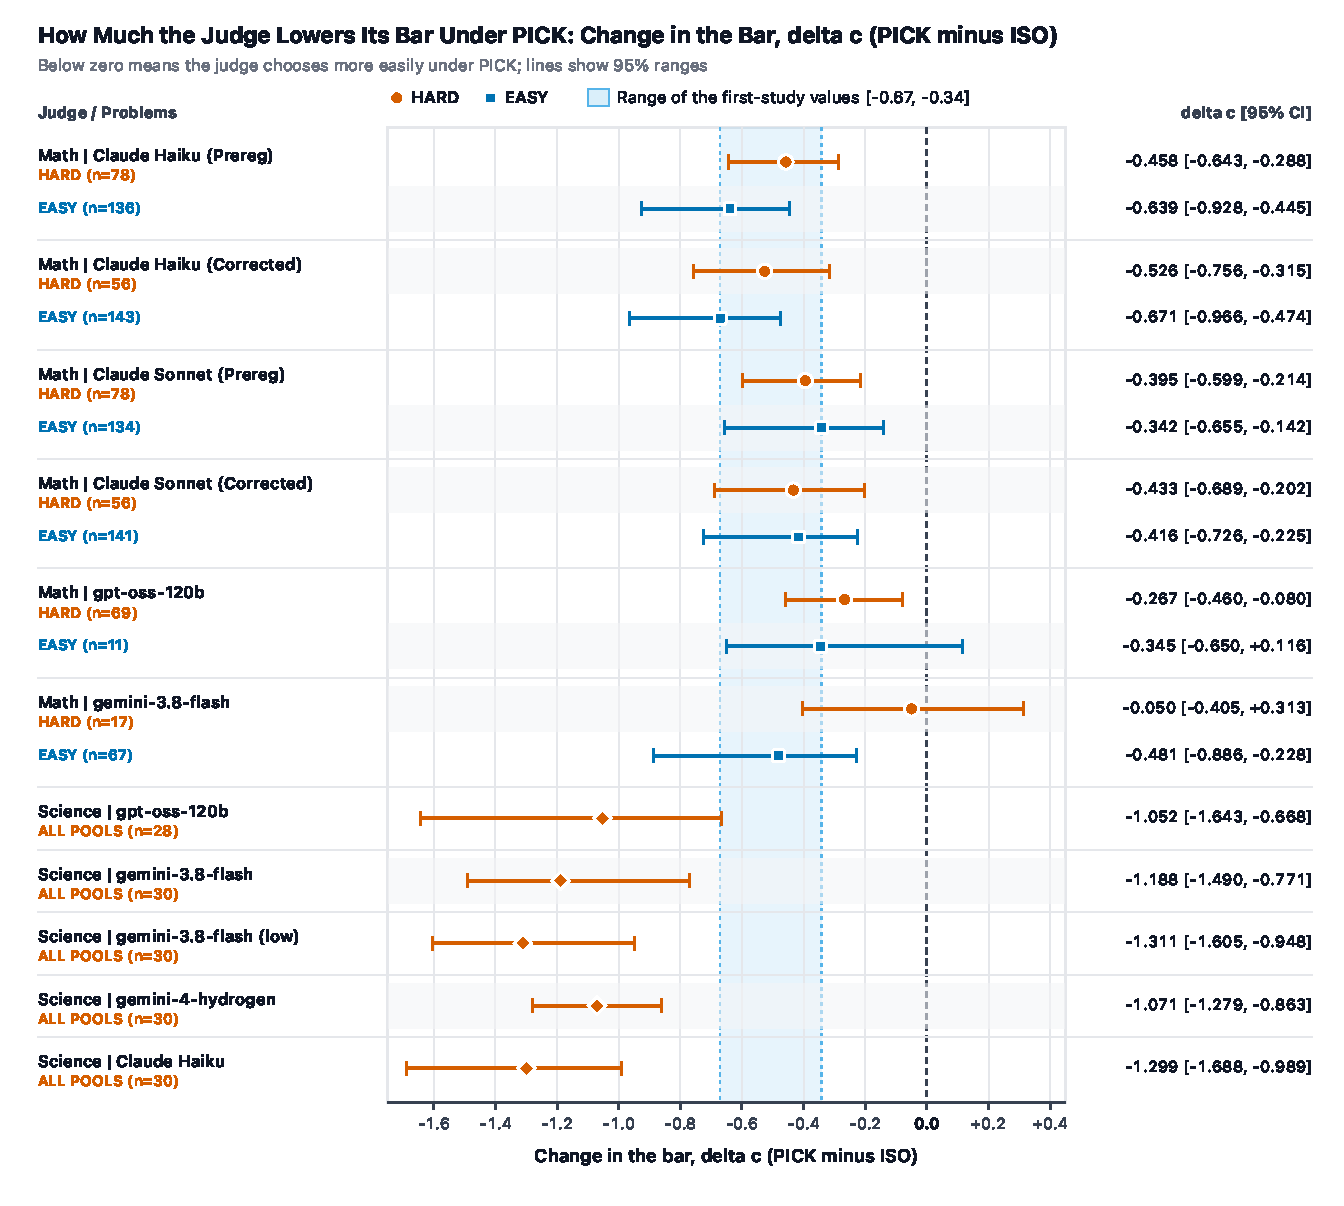
\includegraphics[width=0.92\textwidth]{figures/fig1_criterion_shift}
\caption{Change in the bar, $\Delta c$ (\texttt{PICK} minus \texttt{ISO}), with \res{lvl95} ranges. Below zero means the judge chooses more easily under \texttt{PICK}. Rows: the first study (two Claude judges; ``Prereg'' is the problem set as planned, ``Corrected'' is the set after label fixes), the new math pools (C6) and the science ideas (C9). The shaded band covers the eight values from the first study. It is only a guide for the eye, not a prediction. The science rows are not split into hard and easy, and their ranges ignore that the 30 pools come from only 10 papers (Table~\ref{tab:science} gives ranges that respect this).}
\label{fig:criterion}
\end{figure*}

\begin{figure*}[t]
\centering
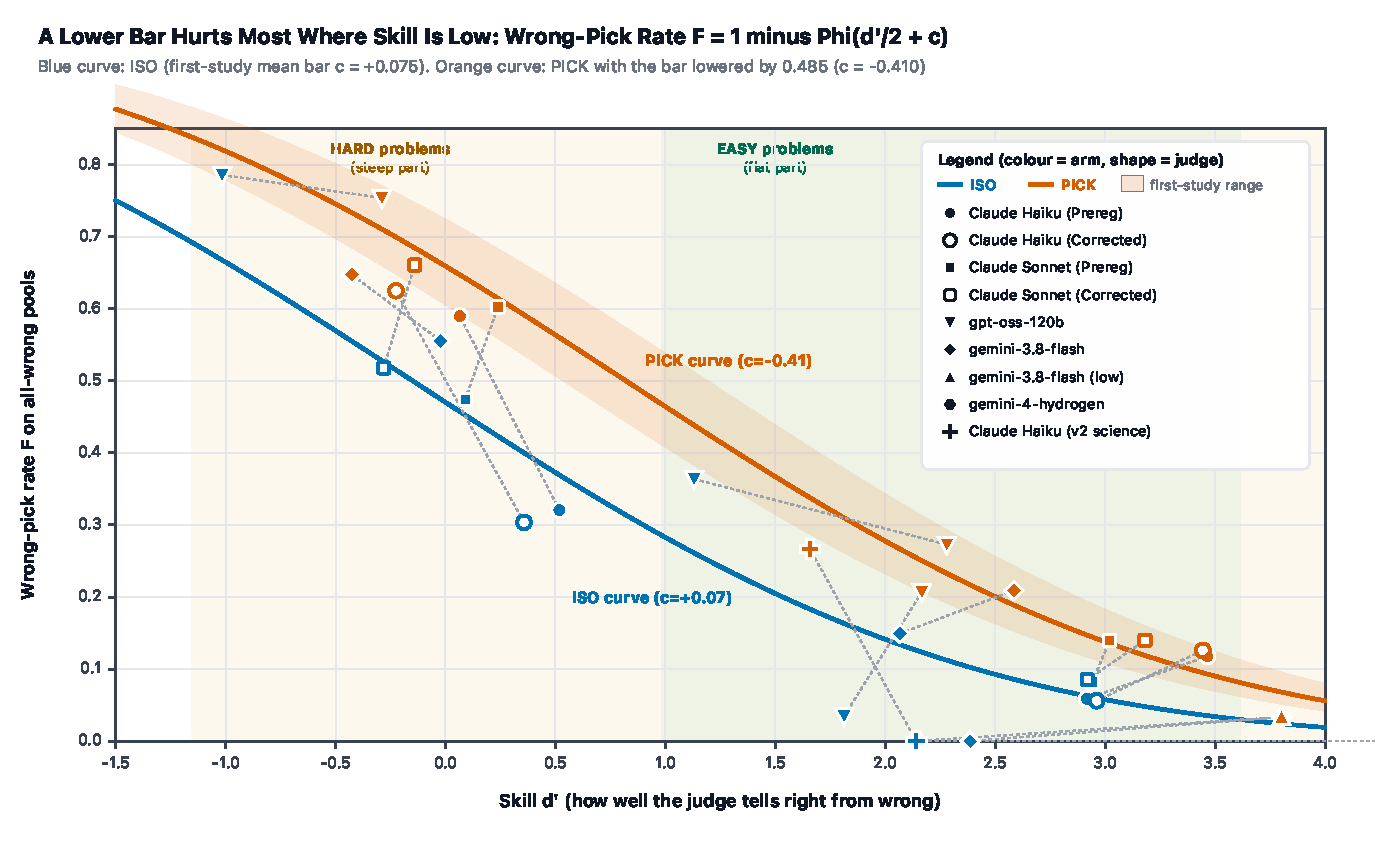
\includegraphics[width=0.92\textwidth]{figures/fig2_sdt_law_curve}
\caption{Why the same lower bar hurts more on hard problems. The curves show the wrong-pick rate $F = 1 - \Phi(d'/2 + c)$ for \texttt{ISO} (blue) and for \texttt{PICK} with a lower bar (orange). On easy problems (high skill, flat right part) the two curves are close, so a lower bar adds few wrong picks. On hard problems (skill near 0, steep left part) the same lower bar adds many. The curves use the average \texttt{ISO} bar and the average $\Delta c$ of the eight cells of the first study, and the shaded band covers the range of those eight $\Delta c$ values. Dotted lines join the \texttt{ISO} and \texttt{PICK} points of one judge and problem group. Several points from the new experiments lie far from both curves. This is how the mixed C6 and C9 results look in a picture.}
\label{fig:sdtlaw}
\end{figure*}

\paragraph{What the first study showed.}
Table~\ref{tab:v1sdt} gives the numbers of the first study (C3) for both Claude judges. In all eight cells the bar is lower under \texttt{PICK}: $\Delta c$ lies between \res{c3sp_s_pi_dc} and \res{c3hc_s_pi_dc}. Skill drops clearly in only one cell, \texttt{claude-haiku-5-5} on hard problems (\res{c3hc_u_pi_ddp}, \res{c3hc_u_pi_ddp_ci}). For \texttt{claude-sonnet-5-5} on hard problems (\res{c3sc_u_pi_ddp}, \res{c3sc_u_pi_ddp_ci}) and for both judges on easy problems, the ranges include zero. So the gap in wrong picks looks larger on hard problems because of where those problems sit on the curve in Figure~\ref{fig:sdtlaw}, not because easy problems escape the lower bar. We formed this explanation after looking at the first study. The first study is therefore only the starting point, and the new experiments are the real tests.

\begin{table*}[t]
\centering\footnotesize
\setlength{\tabcolsep}{4.5pt}
\begin{tabular}{llrrrrr}
\toprule
 & & & \multicolumn{2}{c}{Wrong-pick rate} & Change in skill & Change in bar \\
Judge & Problems (set) & $N$ & \texttt{ISO} & \texttt{PICK} & $\Delta d'$ [\res{lvl95} range] & $\Delta c$ [\res{lvl95} range] \\
\midrule
\texttt{claude-haiku-5-5} & hard (planned) & \res{c3hp_u_pi_n} & \res{c3hp_u_iso_f} & \res{c3hp_u_pick_f} & \res{c3hp_u_pi_ddp} \res{c3hp_u_pi_ddp_ci} & \res{c3hp_u_pi_dc} \res{c3hp_u_pi_dc_ci} \\
\texttt{claude-haiku-5-5} & easy (planned) & \res{c3hp_s_pi_n} & \res{c3hp_s_iso_f} & \res{c3hp_s_pick_f} & \res{c3hp_s_pi_ddp} \res{c3hp_s_pi_ddp_ci} & \res{c3hp_s_pi_dc} \res{c3hp_s_pi_dc_ci} \\
\texttt{claude-haiku-5-5} & hard (corrected) & \res{c3hc_u_pi_n} & \res{c3hc_u_iso_f} & \res{c3hc_u_pick_f} & \res{c3hc_u_pi_ddp} \res{c3hc_u_pi_ddp_ci} & \res{c3hc_u_pi_dc} \res{c3hc_u_pi_dc_ci} \\
\texttt{claude-haiku-5-5} & easy (corrected) & \res{c3hc_s_pi_n} & \res{c3hc_s_iso_f} & \res{c3hc_s_pick_f} & \res{c3hc_s_pi_ddp} \res{c3hc_s_pi_ddp_ci} & \res{c3hc_s_pi_dc} \res{c3hc_s_pi_dc_ci} \\
\midrule
\texttt{claude-sonnet-5-5} & hard (planned) & \res{c3sp_u_pi_n} & \res{c3sp_u_iso_f} & \res{c3sp_u_pick_f} & \res{c3sp_u_pi_ddp} \res{c3sp_u_pi_ddp_ci} & \res{c3sp_u_pi_dc} \res{c3sp_u_pi_dc_ci} \\
\texttt{claude-sonnet-5-5} & easy (planned) & \res{c3sp_s_pi_n} & \res{c3sp_s_iso_f} & \res{c3sp_s_pick_f} & \res{c3sp_s_pi_ddp} \res{c3sp_s_pi_ddp_ci} & \res{c3sp_s_pi_dc} \res{c3sp_s_pi_dc_ci} \\
\texttt{claude-sonnet-5-5} & hard (corrected) & \res{c3sc_u_pi_n} & \res{c3sc_u_iso_f} & \res{c3sc_u_pick_f} & \res{c3sc_u_pi_ddp} \res{c3sc_u_pi_ddp_ci} & \res{c3sc_u_pi_dc} \res{c3sc_u_pi_dc_ci} \\
\texttt{claude-sonnet-5-5} & easy (corrected) & \res{c3sc_s_pi_n} & \res{c3sc_s_iso_f} & \res{c3sc_s_pick_f} & \res{c3sc_s_pi_ddp} \res{c3sc_s_pi_ddp_ci} & \res{c3sc_s_pi_dc} \res{c3sc_s_pi_dc_ci} \\
\bottomrule
\end{tabular}
\caption{The first study (C3). $N$ is the number of problems. ``Planned'' is the problem set as fixed before the study; ``corrected'' is the set after an audit fixed some labels and groups. Ranges come from 5,000 random resamples of the problems. The bar is lower under \texttt{PICK} in all eight rows.}
\label{tab:v1sdt}
\end{table*}

\section{How the New Experiments Were Run}
\label{sec:design}
\paragraph{Fixing the plan first.} Before the judge calls of each experiment, we saved its candidate pools, the program that reads the judges' replies (the parser), two plan documents (\texttt{PREREGISTRATION\_V2.md}, \texttt{PREREG\_C7.md}) and the C7 job files, and we recorded a digital fingerprint (SHA-256) of each in \texttt{LOCKED.sha256}. A changed file would have a different fingerprint. This is a lock on our own computer. We did not deposit the plan with an outside registry. When we say ``planned'' or ``fixed in advance'', we mean exactly this.

\paragraph{Calling the judges.} We called every judge through subscription command-line tools: the Claude CLI for \texttt{claude-haiku-5-5} and the Antigravity CLI for the other judges. Each call started from an empty folder with an instruction not to use tools. The Antigravity tool does not let us switch tools off or remove its own hidden instructions, so for those judges we rely on the instruction.

\paragraph{Computing the numbers.} Two separate programs (\texttt{analysis\_a.py}, \texttt{analysis\_b.py}) computed every number, and we compared their outputs value by value. AI agents in the same project wrote both programs. This protects against coding slips, but less against a wrong idea shared by both. Ranges use 5,000 random resamples of the problems. The $p$ values are one-sided and come from resampling or from the exact McNemar test. We did not correct them for running many tests.

\begin{itemize}\setlength{\itemsep}{2pt}
\item \textbf{C4 (same compute).} On the hard problems of \texttt{claude-haiku-5-5} from the corrected set ($N=\res{c4_n_ta}$ all-wrong pools, $N=\res{c4_n_tp}$ of them with a matching one-right pool; \res{c4_calls_ok}/\res{c4_calls_exp} calls, \res{c4_parse_pct} readable), we run \texttt{PICK} three times per pool. \texttt{PICK\_MAJ3} takes the answer that at least two of the three calls agree on and says \texttt{NONE} if all three differ. \texttt{PICK\_ANY3} counts a wrong pick if any of the three calls picks a candidate. We compare both with \texttt{ISO}, which also uses three calls.
\item \textbf{C5 (removal).} First, we take the $N=\res{c5o_all_n}$ all-wrong pools from the first study in which exactly one candidate has the same answer as Haiku's own attempt ($N=\res{c5o_corr_n}$ after the label audit). We remove that candidate and run \texttt{PICK} on the two that remain (\texttt{PICK-2}). We compare with the stored \texttt{ISO} verdicts for the same two candidates (\texttt{ISO-2}). Second, we follow a classic eyewitness test \citep{wells1993what,wells1984psychology}: in $N=\res{c5w_n}$ all-wrong pools where Haiku picked a wrong candidate in the first study, we remove the picked candidate and run \texttt{PICK-2} on the other two.
\item \textbf{C6 (other judges, new math pools).} $N=\res{c6_n_problems}$ problems (50 contest problems from MathArena and 50 from its arXivMath set). No pool contains a candidate written by a GPT or Gemini model, so no judge sees an answer from its own model family. The position of the correct candidate changes from pool to pool. The judges are \texttt{gpt-oss-120b-medium} and \texttt{gemini-3.8-flash-medium}. Each judge first tries to solve every problem twice. A problem is hard for that judge if both tries are wrong, easy if both are right, and mixed otherwise.
\item \textbf{C9 and C8 (science ideas, less thinking).} From 10 ResearchBench papers \citep{liu2025researchbench} we build $N=\res{c9_n_items}$ all-wrong and $N=\res{c9_n_items}$ one-right pools with four research ideas each. Each paper gives three pools with different wrong ideas. The paper's one true idea is reused in its three one-right pools, and each judge checks it alone only once. Judges: \texttt{gpt-oss-120b-medium}, \texttt{gemini-3.8-flash-medium}, \texttt{gemini-3.8-flash-low} (C8, the same model with less thinking), \texttt{gemini-4-hydrogen-medium} and \texttt{claude-haiku-5-5}.
\item \textbf{C7 (fixes).} Fixed in \texttt{PREREG\_C7.md}. We compare three fixes with plain \texttt{PICK} (called M0) and with \texttt{ISO}. \textbf{M1} (check alone, then pick): run \texttt{ISO} first; if the judge accepts no candidate the answer is \texttt{NONE}, if it accepts one that is the answer, and if it accepts two or more, one extra \texttt{PICK} call chooses among them. \textbf{M2} (error hunt): one call in which the judge must first look for a concrete error in each candidate and then give a confidence from 1 to 5; we keep its pick only at confidence 4 or more. \textbf{M3} (known decoy): we add a wrong solution from a different problem to each pool, in changing positions, to see if rejecting an obvious wrong answer makes the judge stricter. For Haiku on math we use 40 of the 56 paired C4 problems, drawn at random with a fixed seed.
\end{itemize}

\paragraph{What we changed from the plan.}
(i) C4 was planned on the first study's planned set (90 all-wrong, 78 one-right pools), with the corrected set as an extra check. We ran only the corrected set. (ii) In C5 we did not run the planned fresh \texttt{ISO} check or the extra set of 45 pools. (iii) The C6 plan named other judge models and the pools of the first study. We used the two judges that our subscription offered and a new set of pools, locked before its calls. We did not run the planned regression on problem difficulty. (iv) The C6 plan required at least 25 hard and 25 easy problems per judge. Neither judge reaches this (Section~\ref{sec:c6}), so by our own rule the C6 results by difficulty only describe the data and prove nothing. (v) C9 pools have four candidates, not three, and come from 10 papers. Our plan also required that \texttt{ISO} accepts at least some wrong candidates; on C9 only \texttt{gpt-oss-120b-medium} does, because the other four settings accepted no wrong idea when checking alone. (vi) C7 follows the later plan \texttt{PREREG\_C7.md}: 40 problems instead of all, M3 added, and no check on easy problems. (vii) After the lock we found two gaps in the parser. It marked some correct answers as wrong when they were written in a different but equal mathematical form (14 files), and it missed final answers written in bold or without the usual box (10 files from \texttt{gpt-oss-120b-medium}). We did not change the locked parser. An added step handles these cases, and both analysis programs use the same rules. This moves some C6 problems from hard to easy. (viii) The planned check of the first study's labels by a human who does not see the results has not been done.

\section{Results}

\subsection{More Calls for PICK Do Not Close the Gap (C4)}
Three \texttt{PICK} calls and three \texttt{ISO} calls use about the same amount of text written by the judge, counting both its answer and its thinking. Across \res{c4_tok_n} pools the median is \res{c4_tok_pick} vs \res{c4_tok_iso} tokens (a token is a small piece of a word), a ratio of \res{c4_tok_ratio}. We had planned to accept a ratio between 0.90 and 1.10. The ratio is \res{c4_tok_ratio_ta} on all-wrong pools and \res{x_c4_tok_ratio_tp} on one-right pools, so on one-right pools \texttt{PICK} used a little less and falls just outside the planned band.

With compute this close, the gap does not shrink. On the $N=\res{c4_n_ta}$ all-wrong pools, \texttt{PICK\_MAJ3} makes a wrong pick in \res{c4_ta_maj3} (\res{c4_ta_maj3_ci}) of pools. This is the same as a single \texttt{PICK} call (\res{c4_ta_pick1x}, difference \res{c4_d_maj3_p1x}, \res{c4_d_maj3_p1x_ci}) and higher than \texttt{ISO} (\res{c4_ta_iso}) by \res{c4_d_maj3_iso} (\res{c4_d_maj3_iso_ci}, $p$ \res{c4_d_maj3_iso_p}). \texttt{PICK\_ANY3} is worse, with \res{c4_ta_any3} wrong picks (difference from \texttt{ISO} \res{c4_d_any3_iso}, \res{c4_d_any3_iso_ci}). On the $N=\res{c4_n_tp}$ problems that have both pool types, \texttt{PICK\_MAJ3} lowers the bar by \res{c4_sdtd_maj3_iso_dc} (\res{c4_sdtd_maj3_iso_dc_ci}) and lowers skill by \res{c4_sdtd_maj3_iso_ddp} (\res{c4_sdtd_maj3_iso_ddp_ci}) compared with \texttt{ISO}. For this judge and these problems, the extra wrong picks of \texttt{PICK} are therefore not caused by using one call instead of three.

\subsection{Removing the Judge's Own Answer or Its First Pick (C5)}
In the first study, 46 of 90 all-wrong pools for hard problems contained a candidate with the same answer as Haiku's own wrong attempt. Maybe Haiku picks that candidate only because it agrees with itself. We removed it (\res{c5o_ok}/\res{c5o_exp} calls, \res{c5o_parse_pct} readable). A gap remains. Across all \res{c5o_all_n} pools, \texttt{PICK-2} makes a wrong pick in \res{c5o_all_pick2} (\res{c5o_all_pick2_ci}) and \texttt{ISO-2} in \res{c5o_all_iso2} (\res{c5o_all_iso2_ci}), a gap of \res{c5o_all_dc5} (\res{c5o_all_dc5_ci}, $p$ \res{c5o_all_dc5_p}). On the audited subset ($N=\res{c5o_corr_n}$) the gap is \res{c5o_corr_dc5} (\res{c5o_corr_dc5_ci}, $p$ \res{c5o_corr_dc5_p}).

These pools come from the first study, where many candidates were written by Claude models. So we split them. In pools where neither remaining candidate is from Claude ($N=\res{c5o_all_cl0_n}$), \texttt{PICK-2} gives \res{c5o_all_cl0_pick2} and \texttt{ISO-2} gives \res{c5o_all_cl0_iso2}, a gap of \res{c5o_all_cl0_dc5} (\res{c5o_all_cl0_dc5_ci}). In pools with at least one Claude candidate ($N=\res{c5o_all_cl1_n}$), \texttt{PICK-2} gives \res{c5o_all_cl1_pick2} and \texttt{ISO-2} gives \res{c5o_all_cl1_iso2}, a gap of \res{c5o_all_cl1_dc5} (\res{c5o_all_cl1_dc5_ci}). So agreeing with its own answer is not the only cause, but the group without Claude candidates is small.

In the second test ($N=\res{c5w_n}$, \res{c5w_parse_pct} readable) we removed the wrong candidate that Haiku had picked in the first study. Haiku then picked one of the two remaining wrong candidates in \res{c5w_pick2} (\res{c5w_pick2_ci}) of pools. This is more than \texttt{ISO-2} (\res{c5w_iso2}, difference \res{c5w_diff}, \res{c5w_diff_ci}, $p$ \res{c5w_diff_p}). It is also more than the \res{c5w_prop_base} we would expect if two candidates simply drew two thirds of the wrong picks that three candidates drew (difference \res{c5w_vs_prop}). That last comparison is only a rough guide and has no range. The pattern is like the eyewitness result: when the chosen person is taken out of the lineup, many witnesses move to another person and do not say ``not present''.

\subsection{Science Ideas (C9) and Less Thinking (C8)}
Table~\ref{tab:science} and Figure~\ref{fig:crossvendor}(b) show five judge settings on the \res{c9_n_items} all-wrong and \res{c9_n_items} one-right pools of science ideas (1,250 calls; readable replies \res{c9_haiku_parse_pct}, \res{c9_gptoss_parse_pct}, \res{c9_gemini_parse_pct}, \res{c9_gemlow_parse_pct} and \res{c9_hydro_parse_pct}, in the order of the table). The bar is lower under \texttt{PICK} for every setting. This also holds when we resample the 10 papers and not the 30 pools. But the reason differs from judge to judge, and the sample is small.

\begin{table*}[t]
\centering\footnotesize
\setlength{\tabcolsep}{4pt}
\resizebox{\textwidth}{!}{%
\begin{tabular}{lrrrrrrr}
\toprule
 & \multicolumn{3}{c}{Wrong picks (all-wrong pools)} & \multicolumn{2}{c}{Right picks (one-right pools)} & \multicolumn{2}{c}{Change in bar $\Delta c$} \\
Judge (science ideas, $N=\res{c9_n_items}$) & \texttt{ISO} & \texttt{EACH} & \texttt{PICK} & \texttt{ISO} & \texttt{PICK} & [range, by pool] & [range, by paper] \\
\midrule
\texttt{claude-haiku-5-5} & \res{c9_haiku_ta_iso} & \res{c9_haiku_ta_each} & \res{c9_haiku_ta_pick} & \res{c9_haiku_tp_iso} & \res{c9_haiku_tp_pick} & \res{c9_haiku_pi_dc} \res{c9_haiku_pi_dc_ci} & \res{x_c9_haiku_dc_ci} \\
\texttt{gpt-oss-120b-medium} & \res{c9_gptoss_ta_iso} & \res{c9_gptoss_ta_each} & \res{c9_gptoss_ta_pick} & \res{c9_gptoss_tp_iso} & \res{c9_gptoss_tp_pick} & \res{c9_gptoss_pi_dc} \res{c9_gptoss_pi_dc_ci} & \res{x_c9_gptoss_dc_ci} \\
\texttt{gemini-3.8-flash-medium} & \res{c9_gemini_ta_iso} & \res{c9_gemini_ta_each} & \res{c9_gemini_ta_pick} & \res{c9_gemini_tp_iso} & \res{c9_gemini_tp_pick} & \res{c9_gemini_pi_dc} \res{c9_gemini_pi_dc_ci} & \res{x_c9_gemini_dc_ci} \\
\texttt{gemini-3.8-flash-low} (C8) & \res{c9_gemlow_ta_iso} & \res{c9_gemlow_ta_each} & \res{c9_gemlow_ta_pick} & \res{c9_gemlow_tp_iso} & \res{c9_gemlow_tp_pick} & \res{c9_gemlow_pi_dc} \res{c9_gemlow_pi_dc_ci} & \res{x_c9_gemlow_dc_ci} \\
\texttt{gemini-4-hydrogen-medium} & \res{c9_hydro_ta_iso} & \res{c9_hydro_ta_each} & \res{c9_hydro_ta_pick} & \res{c9_hydro_tp_iso} & \res{c9_hydro_tp_pick} & \res{c9_hydro_pi_dc} \res{c9_hydro_pi_dc_ci} & \res{x_c9_hydro_dc_ci} \\
\bottomrule
\end{tabular}%
}
\caption{Science ideas (C9): $N=\res{c9_n_items}$ all-wrong and \res{c9_n_items} one-right pools from 10 papers, four ideas per pool. Both ranges are \res{lvl95} ranges for $\Delta c$ (\texttt{PICK} minus \texttt{ISO}). The last column resamples papers; we added it after seeing the data. For the Gemini rows, almost all of $\Delta c$ comes from the one-right pools.}
\label{tab:science}
\end{table*}

For \texttt{claude-haiku-5-5} and \texttt{gpt-oss-120b-medium}, \texttt{PICK} gives more wrong picks than \texttt{ISO}. Haiku goes from \res{c9_haiku_iso_ta_k}/\res{c9_haiku_iso_ta_n} to \res{c9_haiku_pick_ta_k}/\res{c9_haiku_pick_ta_n} ($p$ \res{c9_haiku_mcn_ta_p}; the wrong picks fall in \res{x_c9_haiku_pfa_pick} of the 10 papers). \texttt{gpt-oss-120b-medium} goes from \res{c9_gptoss_iso_ta_k}/\res{c9_gptoss_iso_ta_n} to \res{c9_gptoss_pick_ta_k}/\res{c9_gptoss_pick_ta_n} ($p$ \res{c9_gptoss_mcn_ta_p}, which does not pass the usual 0.05 line; \res{x_c9_gptoss_pfa_pick} papers). The three Gemini settings make almost no wrong picks with either method (\res{c9_gemini_iso_ta_k}/\res{c9_gemini_iso_ta_n} to \res{c9_gemini_pick_ta_k}/\res{c9_gemini_pick_ta_n}, \res{c9_gemlow_iso_ta_k}/\res{c9_gemlow_iso_ta_n} to \res{c9_gemlow_pick_ta_k}/\res{c9_gemlow_pick_ta_n}, and \res{c9_hydro_iso_ta_k}/\res{c9_hydro_iso_ta_n} to \res{c9_hydro_pick_ta_k}/\res{c9_hydro_pick_ta_n}).

On one-right pools, every judge finds the true idea much more often under \texttt{PICK}. Checking alone, the judges accepted the true idea for only \res{x_c9_haiku_gold}, \res{x_c9_gptoss_gold}, \res{x_c9_gemini_gold}, \res{x_c9_gemlow_gold} and \res{x_c9_hydro_gold} of the 10 papers (in the order of the table). Under \texttt{PICK} they chose it in \res{c9_haiku_pick_tp_k}, \res{c9_gptoss_pick_tp_k}, \res{c9_gemini_pick_tp_k}, \res{c9_gemlow_pick_tp_k} and \res{c9_hydro_pick_tp_k} of \res{c9_gemini_pick_tp_n} pools. Each true idea was checked alone only once and then reused in three pools, so the \texttt{ISO} rate on one-right pools rests on only 10 verdicts per judge. Tests that treat the 30 pools as separate would make the evidence look stronger than it is, so we do not report them.

For the Gemini settings, the lower bar therefore means more right picks at almost no cost in wrong picks. The small correction for rates of 0 and 1 also makes their $\Delta c$ look larger. On these pools \texttt{PICK} was simply the better method for those judges. This fits our explanation, because a lower bar costs little when skill is high. It also shows that checking alone has a real cost: the judge misses correct candidates. Giving \texttt{gemini-3.8-flash} less thinking (C8) changes its \texttt{ISO} result for one paper and does not change \texttt{PICK}.

\begin{figure*}[t]
\centering
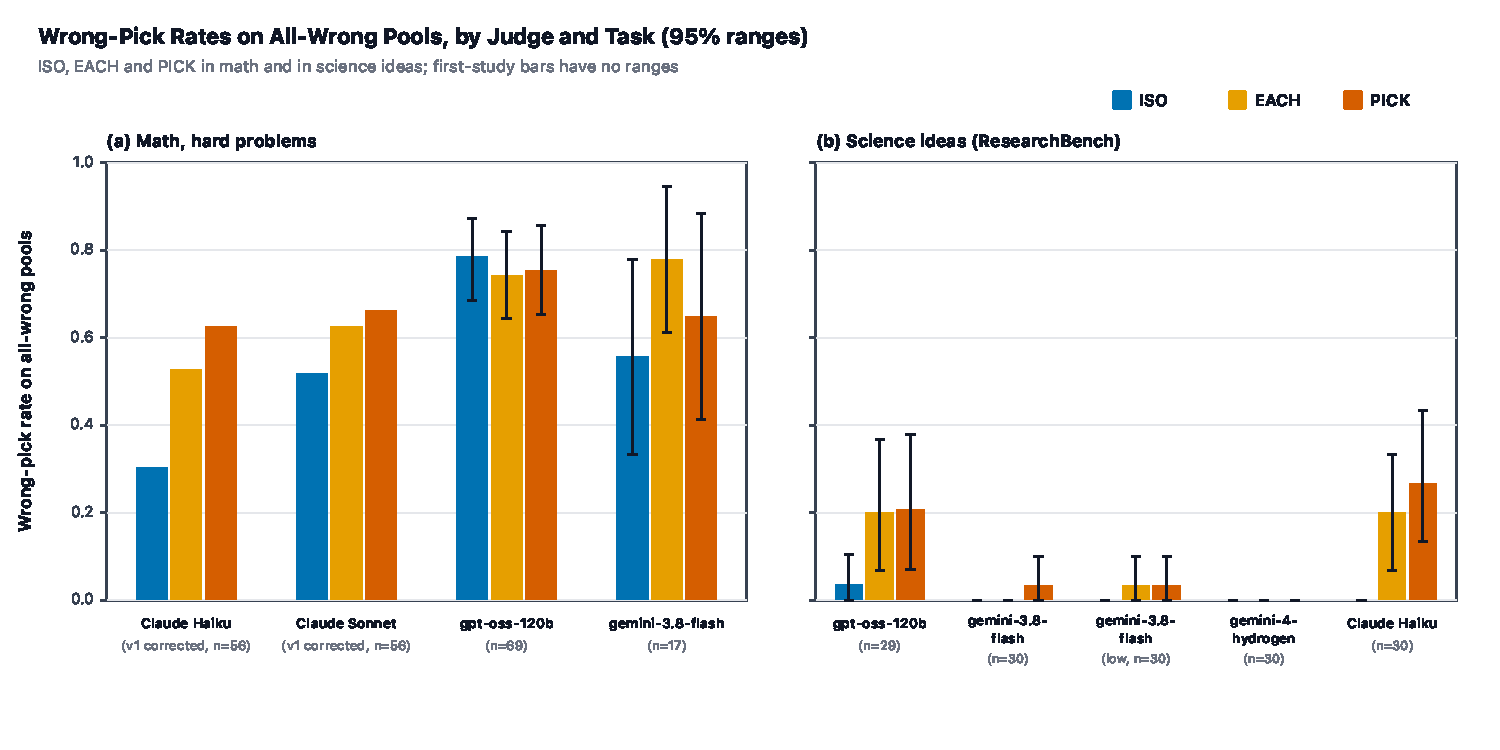
\includegraphics[width=0.95\textwidth]{figures/fig3_crossvendor_domains}
\caption{Wrong-pick rates on all-wrong pools for \texttt{ISO}, \texttt{EACH} and \texttt{PICK}, with \res{lvl95} ranges. (a) Math, the hard problems of each judge. The Claude bars come from the first study, whose pools include candidates from Claude models; we show them without ranges. The other two judges use the new C6 pools. (b) Science ideas, five judge settings.}
\label{fig:crossvendor}
\end{figure*}

\subsection{Judges From Other Companies on New Math Pools (C6)}
\label{sec:c6}
Table~\ref{tab:c6math} shows the math results for the two other judges (1,000 calls per judge; \res{c6_gptoss_parse_pct} readable for \texttt{gpt-oss-120b-medium} and \res{c6_gemini_parse_pct} for \texttt{gemini-3.8-flash-medium}). The two judges split the problems very differently. For \texttt{gpt-oss-120b-medium}, \res{c6_gptoss_n_u} problems are hard (\res{c6_gptoss_n_u_contest} contest, \res{c6_gptoss_n_u_arxiv} arXivMath) and \res{c6_gptoss_n_s} are easy. For \texttt{gemini-3.8-flash-medium}, \res{c6_gemini_n_u} are hard (\res{c6_gemini_n_u_contest} contest, \res{c6_gemini_n_u_arxiv} arXivMath) and \res{c6_gemini_n_s} are easy. Neither judge has 25 problems in both groups, so both miss our minimum group size, and the rows by difficulty only describe the data. The $N$ column of Table~\ref{tab:c6math} counts the problems that enter the \texttt{PICK} minus \texttt{ISO} comparison. This is one fewer than the group size in three rows, and 98 of 100 overall.

\paragraph{Our main planned test fails.} We had planned to test whether \texttt{PICK} gives more wrong picks than \texttt{ISO} on the hard problems of each judge. For \texttt{gpt-oss-120b-medium} the difference is \res{c6_gptoss_u_pi_df} (\res{c6_gptoss_u_pi_df_ci}), with \texttt{ISO} at \res{c6_gptoss_u_ta_iso} and \texttt{PICK} at \res{c6_gptoss_u_ta_pick}. Over all problems it is \res{c6_gptoss_all_pi_df} (\res{c6_gptoss_all_pi_df_ci}). For \texttt{gemini-3.8-flash-medium} it is \res{c6_gemini_u_pi_df} (\res{c6_gemini_u_pi_df_ci}) on hard problems and \res{c6_gemini_all_pi_df} (\res{c6_gemini_all_pi_df_ci}) over all problems. On hard problems, where we planned the test, both ranges include zero. Only the difference over all problems for \texttt{gemini-3.8-flash-medium} is at the edge (its range starts at zero), and for \texttt{gpt-oss-120b-medium} the difference even points the other way. The extra wrong picks that we saw for the Claude judges are at most weakly present here.

\paragraph{The bar is still lower overall.} Over all problems, $\Delta c$ is \res{c6_gptoss_all_pi_dc} (\res{c6_gptoss_all_pi_dc_ci}) for \texttt{gpt-oss-120b-medium} and \res{c6_gemini_all_pi_dc} (\res{c6_gemini_all_pi_dc_ci}) for \texttt{gemini-3.8-flash-medium}. For both judges the lower bar shows mostly as more right picks on one-right pools (\res{c6_gptoss_all_tp_iso} to \res{c6_gptoss_all_tp_pick}, and \res{c6_gemini_all_tp_iso} to \res{c6_gemini_all_tp_pick}). By difficulty the picture is uneven. For \texttt{gpt-oss-120b-medium}, $\Delta c$ is \res{c6_gptoss_u_pi_dc} (\res{c6_gptoss_u_pi_dc_ci}) on hard problems and \res{c6_gptoss_s_pi_dc} (\res{c6_gptoss_s_pi_dc_ci}, $N=\res{c6_gptoss_s_pi_n}$) on easy ones. For \texttt{gemini-3.8-flash-medium} it is \res{c6_gemini_s_pi_dc} (\res{c6_gemini_s_pi_dc_ci}) on easy problems and \res{c6_gemini_u_pi_dc} (\res{c6_gemini_u_pi_dc_ci}, $N=\res{c6_gemini_u_pi_n}$) on hard ones, where the range is wide and centered near zero.

Why do wrong picks not rise for \texttt{gpt-oss-120b-medium}? When it checks candidates alone, it accepts \res{c6_gptoss_cal_w} of the wrong ones (\texttt{gemini-3.8-flash-medium} accepts \res{c6_gemini_cal_w}). With three candidates per pool, \texttt{ISO} then already accepts some wrong candidate in most all-wrong pools. There is little room left for \texttt{PICK} to be worse.

\paragraph{A prediction test.} Our plan included one test with numbers. Take the change in the bar that a judge shows on its easy problems. Apply it to the same judge's \texttt{ISO} bar on hard problems. Then use $F = 1 - \Phi(d'/2 + c)$ to predict the \texttt{PICK} wrong-pick rate on hard problems. For \texttt{gpt-oss-120b-medium} the prediction is \res{x_h3_gptoss_pred}, and we observed \res{c6_gptoss_u_pick_f} (\res{c6_gptoss_u_pick_f_ci}); the prediction lies outside the range. For \texttt{gemini-3.8-flash-medium} the prediction is \res{x_h3_gemini_pred}, and we observed \res{c6_gemini_u_pick_f} (\res{c6_gemini_u_pick_f_ci}); it lies inside, but with only $N=\res{c6_gemini_u_pi_n}$ problems the range is too wide to mean much. Both tests use a group that is smaller than our minimum. Our reading: outside the Claude judges, we have no evidence yet that the bar drops by the same amount on easy and hard problems. We computed this test at the end, with a separate program.

\begin{table*}[t]
\centering\footnotesize
\setlength{\tabcolsep}{4.5pt}
\begin{tabular}{llrrrrrr}
\toprule
 & & & \multicolumn{2}{c}{Wrong picks (all-wrong)} & \multicolumn{2}{c}{Right picks (one-right)} & Change in bar \\
Judge (C6 math) & Problems & $N$ & \texttt{ISO} & \texttt{PICK} & \texttt{ISO} & \texttt{PICK} & $\Delta c$ [\res{lvl95} range] \\
\midrule
\texttt{gpt-oss-120b-medium} & all & \res{c6_gptoss_all_pi_n} & \res{c6_gptoss_all_ta_iso} & \res{c6_gptoss_all_ta_pick} & \res{c6_gptoss_all_tp_iso} & \res{c6_gptoss_all_tp_pick} & \res{c6_gptoss_all_pi_dc} \res{c6_gptoss_all_pi_dc_ci} \\
\texttt{gpt-oss-120b-medium} & hard & \res{c6_gptoss_u_pi_n} & \res{c6_gptoss_u_ta_iso} & \res{c6_gptoss_u_ta_pick} & \res{c6_gptoss_u_tp_iso} & \res{c6_gptoss_u_tp_pick} & \res{c6_gptoss_u_pi_dc} \res{c6_gptoss_u_pi_dc_ci} \\
\texttt{gpt-oss-120b-medium} & easy & \res{c6_gptoss_s_pi_n} & \res{c6_gptoss_s_ta_iso} & \res{c6_gptoss_s_ta_pick} & \res{c6_gptoss_s_tp_iso} & \res{c6_gptoss_s_tp_pick} & \res{c6_gptoss_s_pi_dc} \res{c6_gptoss_s_pi_dc_ci} \\
\midrule
\texttt{gemini-3.8-flash-medium} & all & \res{c6_gemini_all_pi_n} & \res{c6_gemini_all_ta_iso} & \res{c6_gemini_all_ta_pick} & \res{c6_gemini_all_tp_iso} & \res{c6_gemini_all_tp_pick} & \res{c6_gemini_all_pi_dc} \res{c6_gemini_all_pi_dc_ci} \\
\texttt{gemini-3.8-flash-medium} & hard & \res{c6_gemini_u_pi_n} & \res{c6_gemini_u_ta_iso} & \res{c6_gemini_u_ta_pick} & \res{c6_gemini_u_tp_iso} & \res{c6_gemini_u_tp_pick} & \res{c6_gemini_u_pi_dc} \res{c6_gemini_u_pi_dc_ci} \\
\texttt{gemini-3.8-flash-medium} & easy & \res{c6_gemini_s_pi_n} & \res{c6_gemini_s_ta_iso} & \res{c6_gemini_s_ta_pick} & \res{c6_gemini_s_tp_iso} & \res{c6_gemini_s_tp_pick} & \res{c6_gemini_s_pi_dc} \res{c6_gemini_s_pi_dc_ci} \\
\bottomrule
\end{tabular}
\caption{Other judges on new math pools (C6): $N=\res{c6_n_problems}$ problems, half contest and half arXivMath, with no candidate from the judge's own model family. The hard and easy rows only describe the data, because both judges miss the minimum group size. Our files call these groups UNSOLVED\_M and SOLVED\_M.}
\label{tab:c6math}
\end{table*}

\subsection{Three Fixes (C7)}
Table~\ref{tab:mitigation} and Figure~\ref{fig:mitigation} compare the three fixes on the same $N=\res{c7_m1_n}$ hard math problems for \texttt{claude-haiku-5-5}. They also show M2 on the C6 math pools and on the science ideas.

One warning applies to every Haiku math number in this section. We drew the 40 problems at random, with a fixed seed, without looking at results. But the draw was lucky for \texttt{ISO}. In the 40 chosen all-wrong pools, the stored \texttt{ISO} verdicts accept a wrong candidate in \res{x_c7_sub_k} pools. In the \res{x_c7_rest_n} pools that were left out, they do so in \res{x_c7_rest_k}. On the full set it is \res{x_c7_full_k} of \res{x_c7_full_n}, or \res{x_c7_full_f}. The chance of a draw this low is \res{x_c7_tail}. The \texttt{PICK} rate on the 40 problems is the same as on the full set. So the gap between \texttt{PICK} and anything built on \texttt{ISO} is probably too large here. The C4 result on the full set (\res{c4_d_maj3_iso}) is the better guide to the true size.

\begin{figure*}[t]
\centering
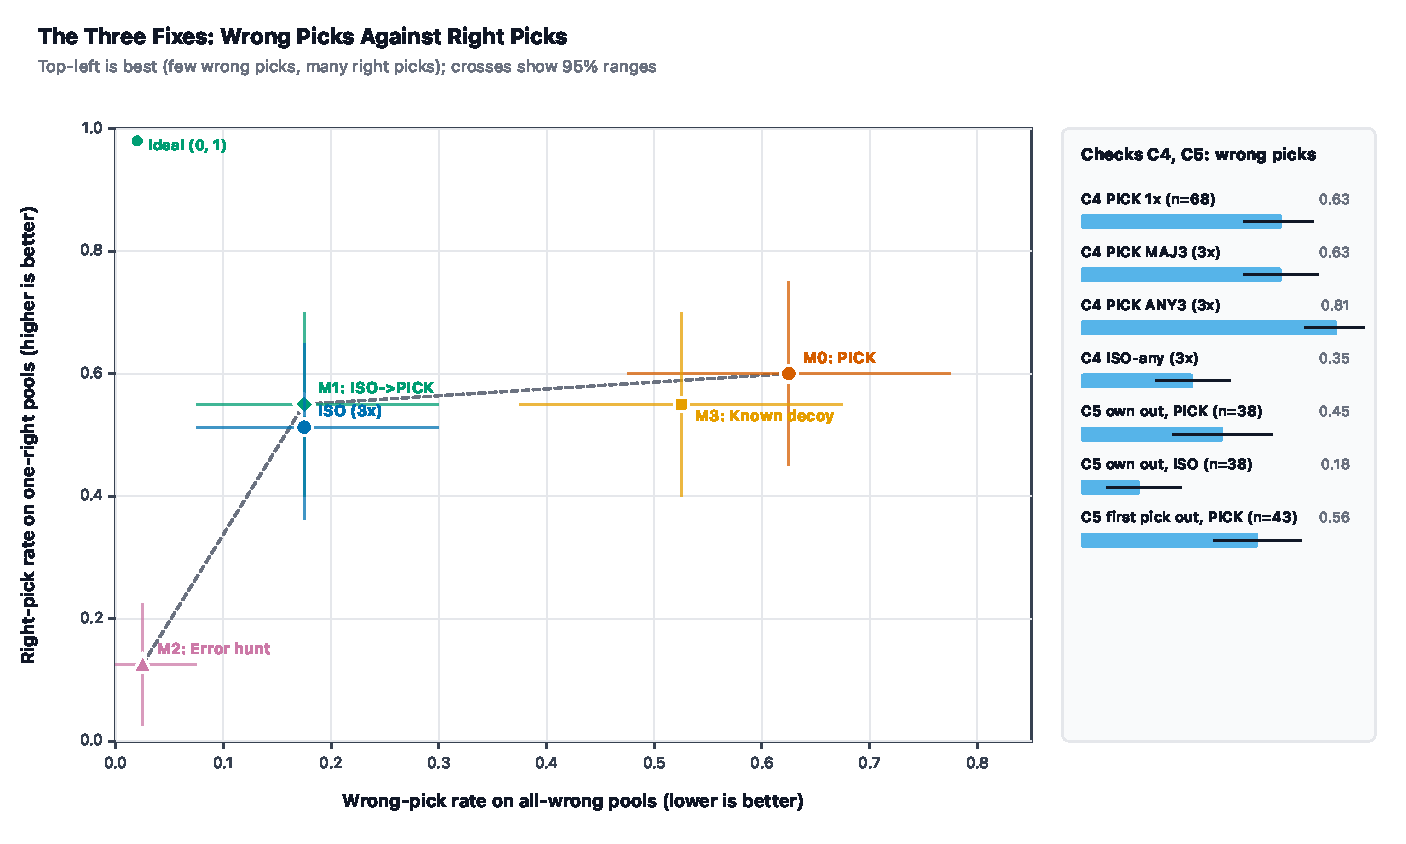
\includegraphics[width=0.94\textwidth]{figures/fig4_mitigation_frontier}
\caption{The fixes on the 40 hard math problems for \texttt{claude-haiku-5-5}: wrong-pick rate on all-wrong pools against right-pick rate on one-right pools, with \res{lvl95} ranges shown as crosses. The best place is the top left. M1 and \texttt{ISO} have the same wrong-pick rate. Right panel: wrong-pick rates in the C4 and C5 checks.}
\label{fig:mitigation}
\end{figure*}

\begin{table*}[t]
\centering\footnotesize
\setlength{\tabcolsep}{3.5pt}
\resizebox{\textwidth}{!}{%
\begin{tabular}{llrrrrr}
\toprule
Task and judge & Method & $N$ & Wrong picks & Right picks & Skill $d'$ [\res{lvl95} range] & Bar $c$ [\res{lvl95} range] \\
\midrule
Hard math, \texttt{claude-haiku-5-5} & M0 (plain \texttt{PICK}) & \res{c7_m1_n} & \res{c7_m1_pick_f} & \res{c7_m1_pick_h} & \res{c7_m1_pick_dp} \res{c7_m1_pick_dp_ci} & \res{c7_m1_pick_c} \res{c7_m1_pick_c_ci} \\
Hard math, \texttt{claude-haiku-5-5} & \texttt{ISO} (3 calls) & \res{c7_m1_n} & \res{c7_m1_iso_f} & \res{c7_m1_iso_h} & \res{c7_m1_iso_dp} \res{c7_m1_iso_dp_ci} & \res{c7_m1_iso_c} \res{c7_m1_iso_c_ci} \\
Hard math, \texttt{claude-haiku-5-5} & \textbf{M1 (check alone, then pick)} & \res{c7_m1_n} & \res{c7_m1_m1_f} & \res{c7_m1_m1_h} & \res{c7_m1_m1_dp} \res{c7_m1_m1_dp_ci} & \res{c7_m1_m1_c} \res{c7_m1_m1_c_ci} \\
Hard math, \texttt{claude-haiku-5-5} & M2 (error hunt) & \res{c7_m2h_n} & \res{c7_m2h_g4_f} & \res{c7_m2h_g4_h} & \res{c7_m2h_g4_dp} \res{c7_m2h_g4_dp_ci} & \res{c7_m2h_g4_c} \res{c7_m2h_g4_c_ci} \\
Hard math, \texttt{claude-haiku-5-5} & M3 (known decoy) & \res{c7_m3_n} & \res{c7_m3_f} & \res{c7_m3_h} & \res{c7_m3_dp} \res{c7_m3_dp_ci} & \res{c7_m3_c} \res{c7_m3_c_ci} \\
\midrule
C6 math, \texttt{gpt-oss-120b-medium} & M2 (error hunt) & \res{c7_m2m_gptoss_n} & \res{c7_m2m_gptoss_g4_f} & \res{c7_m2m_gptoss_g4_h} & \res{c7_m2m_gptoss_g4_dp} \res{c7_m2m_gptoss_g4_dp_ci} & \res{c7_m2m_gptoss_g4_c} \res{c7_m2m_gptoss_g4_c_ci} \\
C6 math, \texttt{gemini-3.8-flash-medium} & M2 (error hunt) & \res{c7_m2m_gemini_n} & \res{c7_m2m_gemini_g4_f} & \res{c7_m2m_gemini_g4_h} & \res{c7_m2m_gemini_g4_dp} \res{c7_m2m_gemini_g4_dp_ci} & \res{c7_m2m_gemini_g4_c} \res{c7_m2m_gemini_g4_c_ci} \\
\midrule
Science, \texttt{claude-haiku-5-5} & M2 (error hunt) & \res{c9_n_items} & \res{c7_m2s_haiku_g4_f} & \res{c7_m2s_haiku_g4_h} & \res{c7_m2s_haiku_g4_dp} \res{c7_m2s_haiku_g4_dp_ci} & \res{c7_m2s_haiku_g4_c} \res{c7_m2s_haiku_g4_c_ci} \\
Science, \texttt{gpt-oss-120b-medium} & M2 (error hunt) & \res{c9_n_items} & \res{c7_m2s_gptoss_g4_f} & \res{c7_m2s_gptoss_g4_h} & \res{c7_m2s_gptoss_g4_dp} \res{c7_m2s_gptoss_g4_dp_ci} & \res{c7_m2s_gptoss_g4_c} \res{c7_m2s_gptoss_g4_c_ci} \\
Science, \texttt{gemini-3.8-flash-medium} & M2 (error hunt) & \res{c9_n_items} & \res{c7_m2s_gemini_g4_f} & \res{c7_m2s_gemini_g4_h} & \res{c7_m2s_gemini_g4_dp} \res{c7_m2s_gemini_g4_dp_ci} & \res{c7_m2s_gemini_g4_c} \res{c7_m2s_gemini_g4_c_ci} \\
Science, \texttt{gemini-3.8-flash-low} & M2 (error hunt) & \res{c9_n_items} & \res{c7_m2s_gemlow_g4_f} & \res{c7_m2s_gemlow_g4_h} & \res{c7_m2s_gemlow_g4_dp} \res{c7_m2s_gemlow_g4_dp_ci} & \res{c7_m2s_gemlow_g4_c} \res{c7_m2s_gemlow_g4_c_ci} \\
Science, \texttt{gemini-4-hydrogen-medium} & M2 (error hunt) & \res{c9_n_items} & \res{c7_m2s_hydro_g4_f} & \res{c7_m2s_hydro_g4_h} & \res{c7_m2s_hydro_g4_dp} \res{c7_m2s_hydro_g4_dp_ci} & \res{c7_m2s_hydro_g4_c} \res{c7_m2s_hydro_g4_c_ci} \\
\bottomrule
\end{tabular}%
}
\caption{The fixes (C7). ``Wrong picks'' is the rate on all-wrong pools and ``right picks'' the rate on one-right pools. On the Haiku math problems, M1 and \texttt{ISO} have the same wrong-pick rate; M1 differs from \texttt{ISO} only in how it chooses when the judge accepts more than one candidate. Where a judge makes no wrong picks and finds every true idea, all resamples give the same value, so the range has zero width.}
\label{tab:mitigation}
\end{table*}

On the Haiku math problems ($N=\res{c7_m1_n}$) the three fixes behave differently.
\begin{itemize}\setlength{\itemsep}{2pt}
\item \textbf{M1 (check alone, then pick) has the same wrong picks as \texttt{ISO}.} The first step settles 72 of the 80 pools with no extra call (in 48 the judge accepts no candidate, in 24 it accepts one). \res{c7_m1_tb_ok} pools need the extra \texttt{PICK} call. So M1 costs the three \texttt{ISO} calls plus \res{c7_m1_extra_calls} calls per pool on average, against one call for \texttt{PICK}. Its wrong-pick rate is \res{c7_m1_m1_f}, the same as \texttt{ISO} (\res{c7_m1_iso_f}) and lower than \texttt{PICK} (\res{c7_m1_pick_f}; difference \res{c7_m1_mp_df}, \res{c7_m1_mp_df_ci}). Compared with \texttt{PICK} it raises the bar by \res{c7_m1_mp_dc}, which is \res{c7_m1_crec} of the distance between \texttt{PICK} and \texttt{ISO}, and it raises skill from \res{c7_m1_pick_dp} to \res{c7_m1_m1_dp} (difference \res{c7_m1_mp_ddp}, \res{c7_m1_mp_ddp_ci}). Compared with \texttt{ISO}, its only gain comes from the extra call: right picks are \res{c7_m1_m1_h} vs \res{c7_m1_iso_h} (difference \res{c7_m1_mi_dh}, \res{c7_m1_mi_dh_ci}) and the skill difference is \res{c7_m1_mi_ddp} (\res{c7_m1_mi_ddp_ci}), based on 8 pools. So M1 is \texttt{ISO} with a sensible way to choose among accepted candidates. Its advantage over \texttt{PICK} is the advantage of \texttt{ISO}.
\item \textbf{M2 (error hunt) goes too far on hard math.} On the Haiku math problems M2 cuts wrong picks to \res{c7_m2h_g4_f}, but right picks fall to \res{c7_m2h_g4_h} (from \res{c7_m1_iso_h} with \texttt{ISO} and \res{c7_m1_pick_h} with \texttt{PICK}). Its bar is very high ($c = \res{c7_m2h_g4_c}$). Its skill (\res{c7_m2h_g4_dp}) is above \texttt{PICK} but not above \texttt{ISO}. So it gives nothing that \texttt{ISO} does not give with far more right picks. On science ideas it also removes Haiku's wrong picks (\res{c9_haiku_ta_pick} to \res{c7_m2s_haiku_g4_f}) and loses right picks (\res{c9_haiku_tp_pick} to \res{c7_m2s_haiku_g4_h}). For \texttt{gpt-oss-120b-medium} on science ideas it roughly halves wrong picks (\res{c9_gptoss_ta_pick} to \res{c7_m2s_gptoss_g4_f}), with right picks at \res{c7_m2s_gptoss_g4_h} (\res{c9_gptoss_tp_pick} with \texttt{PICK}). The Gemini settings already made almost no wrong picks. On the C6 math pools M2 gives \res{c7_m2m_gptoss_g4_f} wrong picks and \res{c7_m2m_gptoss_g4_h} right picks for \texttt{gpt-oss-120b-medium}, and \res{c7_m2m_gemini_g4_f} and \res{c7_m2m_gemini_g4_h} for \texttt{gemini-3.8-flash-medium}. What this fix does depends strongly on the judge and the task.
\item \textbf{M3 (known decoy) does not help.} Haiku never picked the added decoy (\res{c7_m3_foil_all} across 80 pools), so it did read the pool with care. But wrong picks on the three real wrong candidates stayed at \res{c7_m3_f} (difference from \texttt{PICK} \res{c7_m3_mp_df}, \res{c7_m3_mp_df_ci}, a range that includes zero), and the bar stayed well below \texttt{ISO} ($\Delta c$ against \texttt{ISO} \res{c7_m3_mi_dc}). Rejecting an obvious wrong answer did not make the judge stricter about wrong answers that look good.
\end{itemize}

\section{Limits of This Study}
\begin{enumerate}\setlength{\itemsep}{2pt}
\item \textbf{The explanation came after the first data.} We formed the lower-bar explanation after seeing the first study. In the new experiments its direction holds in most cells. But outside the Claude judges we have not shown that the bar drops by the same amount on easy and hard problems, and our one planned prediction with numbers failed (Section~\ref{sec:c6}).
\item \textbf{One judge carries the checks.} C4, C5 and the fixes M1 and M3 use only \texttt{claude-haiku-5-5}, on pools from the first study, where most pools contain a candidate from a Claude model. The C5 group without Claude candidates is small ($N=\res{c5o_all_cl0_n}$) and its range touches zero.
\item \textbf{The science sample is small.} C9 has 30 pools of each type from only 10 papers, and each true idea was checked alone once per judge. Ranges computed by pool make the results look more certain than they are; Table~\ref{tab:science} adds ranges computed by paper.
\item \textbf{Uneven groups in C6.} Neither of the two other judges has enough problems in both the hard and the easy group. For \texttt{gemini-3.8-flash-medium}, almost all hard problems come from arXivMath.
\item \textbf{A lucky draw in C7.} In the 40 chosen problems \texttt{ISO} accepts unusually few wrong candidates. This makes every Haiku math comparison with \texttt{PICK} in C7 look larger.
\item \textbf{A ``Final answer:'' line shown to judges.} Each math candidate was shown with a line ``Final answer:'' taken from MathArena's stored answer field. In some pools this line does not match the boxed answer in the solution text (for example a formula turned into a decimal number, or extra digits): 68 of 543 pools in the first study, 17 of 200 C6 pools, 9 of 124 C4 pools and 6 of 81 C5 pools. Our audit found that the labels are not affected: no candidate labelled wrong has a boxed answer equal to the correct answer. But the judges saw a confusing line in those pools, the same in every method. We have not rerun the analysis without these pools.
\item \textbf{Labels were checked by AI.} AI agents decided the label corrections of the first study. A tool for a human check is ready, but no human has done the check. A scripted audit of 120 files found no parser errors in the C6, C9 and C7 M2 replies after the added step described in Section~\ref{sec:design}.
\item \textbf{Hidden instructions in the tools.} The subscription tools add their own hidden instructions to each call. C4 matches the text the judge writes, not everything the judge reads, and we could not run a control through a plain API.
\item \textbf{Scope.} The results hold for the named model versions and thinking settings, in November 2026, on math problems with short final answers and on choosing among short research ideas.
\end{enumerate}

\section{Conclusion}
For \texttt{claude-haiku-5-5} on hard math, asking the judge to pick among candidates gives more wrong picks on all-wrong pools than checking the candidates one at a time. This stays true when both methods use the same compute, when the judge's own answer is removed, and when its first pick is removed. A lower bar when the judge sees the candidates together describes these data well.

For other judges the picture is mixed. The bar is lower under \texttt{PICK} overall for two other model families on math and for all five settings on science ideas. But for \texttt{gpt-oss-120b-medium} on math the wrong picks do not go up, and for the Gemini judges on science ideas \texttt{PICK} mostly helps.

Of the fixes we tried, only one cut wrong picks on hard math without a clear loss of right picks: checking each candidate alone before any joint choice. It costs about three times the calls.

So the choice between judging together and judging alone depends on two things: how often a pool has no correct candidate, and how well the judge separates right from wrong when it checks alone. Both are cheap to measure with all-wrong pools. In our view, anyone who builds a system with a selection step should measure them before trusting that step.

\section*{Data and code}
The archive of the first study (plans, prompts, raw replies, grading code and analysis programs) is public at \url{https://github.com/chaitshar/when-no-candidate-is-correct/tree/v1.0}. The candidate pools, plan documents, lock files, raw replies, both analysis programs and the final extra program (\texttt{scripts/final\_sensitivity.py}) of this paper are in the \texttt{v2/} folder of the same archive, release v2.0 (\url{https://github.com/chaitshar/when-no-candidate-is-correct/tree/v2.0/v2}). MathArena data carry a CC BY-NC-SA licence.

\section*{Use of AI}
The author set the research direction and the rules. AI coding agents (Google Antigravity and Claude Code) wrote the test programs, ran the experiments and the analysis, and drafted the paper under those rules. An AI agent also checked the draft against the raw replies and the plan documents. This check led to the list of changes from the plan and to several of the limits above. When this paper speaks of ``separate'' programs or checks, it means separate programs written by AI, not checks by a human. The author is responsible for the content.

\bibliographystyle{plainnat}
\bibliography{refs}

\end{document}
